%\documentclass[12pt]{aastex}
\documentclass[iop, numberedappendix]{emulateapj}
%\documentclass{article}
%\usepackage{draftwatermark}
%\usepackage{paralist}
\shorttitle{Vertical shear instability}
\shortauthors{M-K.\ Lin, A.\ N.\ Youdin}

\usepackage{amsmath}
%\usepackage{url}
\usepackage{bm}
%\usepackage[font=small,format=plain,labelfont=bf,up,textfont=it,up]{caption}
\newcommand{\p}{\partial}
\newcommand{\zmax}{z_\mathrm{max}}
\newcommand{\lmax}{l_\mathrm{max}}
\newcommand{\sbar}{\bar{\sigma}} 
\newcommand{\He}{\operatorname{He}}
\newcommand{\imgi}{\mathrm{i}} 
\newcommand{\ii}{\mathrm{i}}
\newcommand{\C}{\mathcal{C}^\lambda}
\newcommand{\wop}[1]{\mathcal{V}^{(#1)}}
\newcommand{\avg}[1]{\langle{#1}\rangle}
%\newcommand{\max}[1]{\mathrm{max}({#1})}
%\newcommand{\min}[1]{\mathrm{min}({#1})}
\newcommand{\zhat}{\hat{z}}
\newcommand{\khat}{\hat{k}}
\newcommand{\rhat}{\hat{r}}
\newcommand{\he}{\mathcal{H}}
\newcommand{\amp}{\mathcal{A}}
\newcommand{\dd}{\delta}
\newcommand{\real}{\operatorname{Re}}
\newcommand{\imag}{\operatorname{Im}}
\newcommand{\sgn}{\operatorname{sgn}}
\newcommand{\wbar}{\tilde{W}}
\newcommand{\qbar}{\tilde{Q}}
\newcommand{\dbigH}{\frac{H^\prime}{H}}
\newcommand{\Rp}{\frac{\rho_0^\prime}{\rho_0}}
\newcommand{\Fp}{\frac{g^\prime}{g}}
\newcommand{\Rpp}{\frac{\rho_0^{\prime\prime}}{\rho_0}}
\newcommand{\Fpp}{\frac{g^{\prime\prime}}{g}}
\newcommand{\ils}{L_s^{-1}}
\newcommand{\ilp}{L_p^{-1}}
\newcommand{\ihp}{H_p^{-1}}
\newcommand{\ihs}{H_s^{-1}}
\newcommand{\ciso}{c_\mathrm{iso}}
\newcommand{\csmid}{c_{s0}} 
\newcommand{\hiso}{h_\mathrm{iso}}
\newcommand{\Hiso}{H_\mathrm{iso}}
\newcommand{\zeus}{\texttt{ZEUS-MP }}
\newcommand{\rsph}{r_\mathrm{sph}}
\newcommand{\dvx}{\dd v_x}
\newcommand{\dvy}{\dd v_y}
\newcommand{\dvz}{\dd v_z}
\newcommand{\dbx}{\dd B_x}
\newcommand{\dby}{\dd B_y}
\newcommand{\dbz}{\dd B_z}
\newcommand{\w}{ \widetilde{W}}
\newcommand{\dphi}{\dd \Phi}
\newcommand{\actaa}{Acta Astron.}
\defcitealias{lin12}{L12} 
\defcitealias{nelson13}{N13}
\defcitealias{barker15}{BL15}
\defcitealias{mcnally14}{MP14}
\defcitealias{goldreich67}{GS67}

\def \OmK {\Omega_{\rm K}}

\begin{document}

\title{Cooling Requirements for the Vertical Shear Instability 
  in Protoplanetary Disks}
%\title{Vertical shear instability in astrophysical disks: vertically
%global linear calculations with thermal relaxation and applications
%to the Solar Nebula}  
\author{Min-Kai Lin\altaffilmark{1} \& Andrew N Youdin}
\affil{Department of Astronomy and Steward Observatory, \\
University of
  Arizona, 933 North Cherry Avenue, Tucson, AZ 85721, USA}
\altaffiltext{1}{Steward Theory Fellow}
\email{minkailin@email.arizona.edu, youdin@email.arizona.edu}

\begin{abstract}
{\bf
The vertical shear instability (VSI) offers a potential hydrodynamic mechanism to drive angular momentum transport in cold protoplanetary disks (PPDs). The VSI is driven by a weak vertical gradient in the disk's orbital motion, but must overcome vertical buoyancy, a strongly
  stabilizing influence in cold disks, where
  heating is dominated by external irradiation.  Rapid radiative cooling      reduces the effective buoyancy
  and allows the VSI to operate.  We quantify the
  cooling timescale, $t_c$, needed for growth of the VSI. We perform a linear analysis of the VSI with cooling in
  vertically global, radially local disk models. We find the VSI is most vigorous for
  rapid cooling with $t_c < \OmK^{-1}  h |q| / (\gamma -1)$
  in terms of the Keplerian orbital frequency, $\OmK$; the disk's
  aspect ratio, $ h \ll 1$; the radial
  power-law temperature gradient, $q$; and the adiabatic index,
  $\gamma$.  For longer $t_c$, the VSI
  is much less effective because growth slows and shifts to smaller length scales, which are more prone to
  viscous or turbulent decay.  We apply our results to PPD models
  where $t_c$ is determined by the opacity of dust grains.  We
  find that the VSI is most effective at intermediate radii, from $\sim 5$AU to $\sim 50$AU with a
  characteristic growth time of $\sim 30$ local orbital periods.
  Growth is suppressed by long cooling times both in the opaque
  inner disk and the optically thin outer disk.  A reduction in the
  dust opacity by a factor of 10 increases cooling times
  enough to quench the VSI at all disk radii.  Thus the formation of
  solid protoplanets, a sink for dust grains, can impede the VSI.
}

%  It is difficult to understand how cold circumstellar disks accrete onto their central stars.  Due to 
%  lower levels of ionization, magnetic transport mechanisms that
%  operate in warmer disks are less effective.  
%  A hydrodynamic mechanism, the vertical shear instability (VSI), offers a means to drive angular momentum 
 % transport in cold accretion disks such as protoplanetary disks (PPDs).  
%  The VSI is driven by a weak vertical gradient in the disk's orbital motion.
%  In order to grow, the VSI must overcome vertical buoyancy, a strongly
%  stabilizing influence in cold disks, where  
%  heating is dominated by external irradiation.  Rapid cooling, via
%  radiative losses, reduces the effective buoyancy 
%  and allows the VSI to operate.  In this paper, we quantify the
%  cooling timescale, $t_c$, needed for growth of the VSI.
%   We perform a linear analysis of the VSI with cooling in
%  vertically global and radially local disk models. 
%  For irradiated disks, we find that the VSI is most vigorous for
%  rapid cooling with $t_c < \OmK^{-1}  h |q| / (\gamma -1)$ 
%  in terms of the Keplerian orbital frequency, $\OmK$; the disk's
%  aspect ratio, $ h \ll 1$; the radial  
%  power-law temperature gradient, $q$; and the adiabatic index,
%  $\gamma$.  For longer cooling times, the VSI  
%  is much less effective because growth slows and shifts to smaller length scales, which are more prone to 
%  viscous or turbulent decay.  We apply our results to PPD models 
%  where $t_c$ is determined by the opacity of dust grains.  We
%  find that the VSI is most effective at intermediate radii, from $\sim 5$AU to $\sim 50$AU with a
%  characteristic growth time of $\sim 30$ local orbital periods.
%  Growth is suppressed by long cooling times both in the opaque  
%  inner disk and the optically thin outer disk.  A reduction in the
%  dust opacity by a factor of 10 increases cooling times  
%  enough to quench the VSI at all disk radii.  Thus the formation of
%  solid protoplanets, a sink for dust grains, can impede the VSI. 
\end{abstract}

\section{Introduction}\label{intro}
Understanding how disks transport mass and angular momentum underlies 
many problems in astrophysics, including star and planet formation  
\citep[][]{armitage10}.  The turbulence associated with many transport mechanisms
is particularly important for dust evolution and planetesimal formation \citep{yl07, chiang10}. 

Magneto-hydrodynamic (MHD) turbulence driven by
the magneto-rotational instability \citep[MRI,][]{balbus91} has long been the most
promising transport mechanism in low mass disks with weak self-gravity. 
However, many parts of protoplanetary  
disks (PPDs) are cold, have low levels of ionization, and do not support the MRI 
\citep{blaes94,salmeron03}. Recent simulations
suggest that significant portions of PPDs fail to develop MHD
turbulence \citep[e.g.][]{simon13, lesur14,bai15,gressel15}. 

A purely hydrodynamic mechanism could circumvent difficulties with non-ideal MHD, but must overcome
the strong centrifugal stability imposed by the positive radial specific angular
momentum gradient in nearly Keplerian disks \citep{balbus96}.
One possible route to hydrodynamic turbulence is the vertical shear
instability (VSI, \citealp{urpin98, urpin03, nelson13}, hereafter \citetalias{nelson13}).  The
basic mechanism of the VSI  in disks was first 
identified in the context of differentially rotating stars (\citealp{goldreich67}, hereafter \citetalias{goldreich67}, \citealp{fricke68}).   
The VSI arises when vertical shear, i.e.\ a variation in orbital motion along the rotation axis, 
destabilizes inertial-gravity waves, which are oscillations 
with rotation and buoyancy as restoring forces. 
% \citep{lubow93}. 
Vertical shear
occurs wherever the disk is baroclinic, i.e.\ when constant 
density and constant pressure surfaces are misaligned.  Baroclinicity, and thus vertical shear, is 
practically unavoidable in astrophysical disks, except at special locations like the
midplane. 

To overcome centrifugal stabilization, the VSI triggers motions which are vertically elongated 
and radially narrow.  %This geometry minimizes the effects of the radial gradient of angular momentum.
Vertical elongation taps the free energy of the vertical shear \citep{umurhan13}, but is also subject to 
the stabilizing effects of vertical buoyancy if the disk is stably
stratified. To overcome vertical buoyancy, the VSI requires a short cooling time
(\citetalias{goldreich67}; \citetalias{nelson13}). Rapid radiative 
cooling, i.e.\ a short thermal relaxation timescale, brings a
moving fluid element into thermal equilibrium with 
its surroundings, thereby diminishing buoyancy. %not obvious actually
                                %- requires assumption of ideal gas
                                %e.o.s. and pressure eqm established
                                %quickly 
An isothermal equation of state implies instantaneous thermal relaxation, and is the ideal context for studying the VSI
(\citealp{urpin03}; \citetalias{nelson13}; \citealp{mcnally14}, hereafter \citetalias{mcnally14}; \citealp{barker15},
hereafter \citetalias{barker15}).    

Alternatively, vertical buoyancy can be eliminated by strong internal
heating, i.e.\ by the onset of convection, so that the disk becomes 
neutrally stratified in the vertical direction
\citepalias{nelson13,barker15}. However, realistic PPDs should be vertically
stably stratified in the outer regions, beyond $\sim 1$--5 AU, where
heating is  irradiation dominated \citep{bitsch15}.  Even in the inner
disk, strong vertical buoyancy is possible if accretion heating is
weak or is concentrated in surface layers \citep{gammie96,lesniak11}.  

Understanding the VSI in real disks therefore requires
considering finite, non-zero cooling times, $t_{\rm c}$. Non-linear
hydrodynamical simulations with a prescribed  $t_{\rm c}$ find that VSI
turbulence in stably stratified disks requires rapid cooling  
with $t_{\rm c}$ shorter than orbital timescales
 \citepalias{nelson13}. When the cooling time is short enough, 
 the VSI can drive moderately strong transport, with Reynolds
stresses of $\alpha \sim 10^{-3}$ times the mean pressure \citepalias{nelson13}. Simulations
with realistic radiative transfer, in lieu of a fixed $t_{\rm
  c}$, find that the VSI in irradiated disks drive transport with
$\alpha \sim 10^{-4}$  in a  $\sim 2$ -- 10AU PPD model \citep{stoll14}.  

Studying the linear growth of the VSI is necessary for 
understanding how it can ultimately drive turbulent transport.
The pioneering linear analyses of the VSI considered vertically 
local disturbances \citep{urpin98,urpin03}.  A vertical global analysis 
(e.g.\ \citetalias{nelson13,mcnally14,barker15}) 
is essential for understanding how vertically elongated disturbances 
interact with the disk's vertical structure.  Moreover a vertically global analysis
allows more direct comparisons with modern numerical simulations.  This work 
generalizes previous vertically global analyses by including a finite cooling time.

%NOTE: no need to reexplain importance of cooling or to say more about our work before the "organized as follows" summary

This paper is organized as follows. In \S\ref{vsi_require} we explain, without derivation,  
our main result for the critical cooling timescale, beyond which VSI growth is 
suppressed. %We then present the  
%formal linear problem in \S\ref{setup}---\ref{numerical}.    
 We develop our disk model in \S\ref{setup} and derive linearized
 perturbation equations in  \S\ref{linear}.
 Section \ref{analytical} contains our main analytic results, leading to 
 the derivation of the critical cooling time in \S\ref{iso_vsi_beta_crit}.
 In \S\ref{numerical} we analyze linear VSI growth, and numerically confirm the critical cooling time.
We apply our results to PPDs in \S\ref{application}, with cooling times derived from dust opacities.
We discuss caveats and extensions in \S\ref{caveats}.
 We conclude in \S\ref{summary} with a summary.  Some technical and background 
 developments are explained in the appendices.  


%The VSI is an axisymmetric linear instability 
%in three-dimensional (3D) disks in which the rotation frequency
%$\Omega$ depends on the height $z$ from the disk midplane. 
%Vertical shear occurs whenever the disk is baroclinic, i.e.\ when constant 
%density and constant pressure surfaces are misaligned.  Baroclinicity, and thus vertical shear, is 
%practically unavoidable in disks, except at special locations like the midplane.
%
%A height-dependence in $\Omega$, or vertical shear, can render
%inertial waves unstable. \cite{barker15} gives a simple 
%interpretation of the VSI: in an axisymmetric, inviscid, neutrally
%stratified disk, the exchange of fluid parcels vertically, while
%conserving their specific angular momentum, can result in a new
%configuration of lower energy if the distribution of specific angular
%momentum varies with $z$. The VSI is characterized by perturbations
%with large vertical length-scales  relative to radial length-scales.   
%
%Early analysis of the VSI in radially and vertically local 
%models of accretion disks \citep{urpin98,urpin03} showed that the VSI
%requires a short thermal timescale so that perturbations evolve 
%isothermally, unless the disk is neutrally stratified in the vertical
%direction. This is because
%vertical motions associated with the VSI 
%are stabilized by buoyancy forces if the disk is sub-adiabatically
%stratified (convectively stable). A sufficiently short thermal
%timescale renders buoyancy ineffective, but a quantitative criteria is
%desirable. This is our primary goal.  
%
%The need for a short thermal timescale for the VSI to operate in
%stably stratified disks has been demonstrated in recent numerical simulations 
%\citep{nelson13,stoll14}. When the  thermal timescale $t_c$ is
%parametrized in units of the orbital period  $P_\mathrm{orb}$,
%\cite{nelson13} find that $t_c\lesssim  0.01P_\mathrm{orb}$ was needed
%to observe the VSI. That is, the  disk temperature needs to remain
%effectively unchanged. Radiation hydrodynamic simulations performed by
%\cite{stoll14} also showed that the VSI is only sustained with the
%inclusion of heating from stellar irradiation, which results in an
%effective thermal timescale $t_c\ll P_\mathrm{orb}$ that maintains a
%fixed temperature profile.     
%
%These studies show that the VSI is generally sensitive to disk
%thermodynamics. It is thus important to quantify this dependence, for
%example on disk parameters, in order to evaluate the relevance of the
%VSI to realistic disks, which one may expect to be stably
%stratified and have non-zero thermal timescales.  In order to determine
%where in the disk the VSI may operate, and hence lead to hydrodynamic
%turbulence, understanding the thermodynamic dependence of the linear VSI is essential. 
%
%In this work we study the linear VSI in radially local, vertically
%global models of astrophysical disks. This approach has
%been adopted in recent studies of the linear VSI
%\citep{nelson13,mcnally14,barker15}. However, these studies consider 
%isothermal perturbations, for which the thermal timescale is formally
%zero, and/or neutrally stratified disks in which buoyancy forces are
%absent by construction. We account for both effects to study the
%VSI in more general disk models. To do so, we examine 
%sub-adiabatically stratified disks and include an energy equation 
%with a source term that allows the thermodynamic response of 
%perturbations to be varied smoothly between isothermal and 
%adiabatic.   
%
%
%This paper is organized as follows. We first highlight in
%\S\ref{vsi_require} the need of a very short thermal timescale for the
%VSI to operate in stably stratified disks. There we also preview our
%main result --- a quantitative thermodynamic criteria for the VSI ---
%and a first application to protoplanetary disks. The remaining sections
%are devoted to deriving these results from linear theory. 
%
%In \S\ref{setup} we list the governing equations and global
%equilibrium disk models under   
%consideration. We formulate the linear stability problem in 
%\S\ref{linear} and simplify it by making the radially local
%approximation. We study the linear problem using two approaches. In
%\S\ref{analytical} we present an analytical discussion of vertically
%isothermal disks. Our treatment is grossly simplified owing to a
%number of approximations made, but closely parallels previous work, 
%allowing us to highlight the essential effects of vertical shear, and to
%derive a characteristic upper limit to the thermal timescale for the
%VSI. This timescale is \emph{much shorter} than the dynamical
%timescale. In \S\ref{numerical} we numerically
%solve the linear problem in the radially local approximation, but
%relax all other approximations made in our analytical approach.    
%We find basic agreement with our analysis, including
%the aforementioned characteristic thermal timescale. 
%
%In
%\S\ref{application} we apply our results to the Minimum Mass
%Solar Nebula (MMSN) by modeling thermal 
%timescales based on realistic disk properties, and find that the VSI
%can operate effectively in the outer parts of the MMSN. We summarize in
%\S\ref{summary} with a discussion of caveats and possible directions
%for future work.  



\section{Why must cooling be so fast?}\label{vsi_require}     
In a stably stratified thin disk, the VSI  
requires a thermal timescale $t_c$ significantly shorter than the
disk dynamical timescale, 
\begin{align}
  t _c \ll \OmK^{-1},
\end{align}
where $\OmK$ is the Keplerian frequency (N13).    
This requirement --- that the cooling time be much shorter than an orbital period, 
which in turn is much smaller than the relevant oscillation period of vertically elongated gravity waves  --- is quite stringent.
It highlights the fact that vertical buoyancy is strongly 
stabilizing. Rapid radiative damping is thus required to weaken
buoyancy and allow the weak vertical shear to drive instability.   

To roughly quantify the required smallness of $t_c$, we consider a
vertically isothermal disk with aspect-ratio $ h$, 
 radial temperature profile $T \propto r^q$ and adiabatic index
$\gamma>1$ so the disk is stably stratified.  For a PPD, $ h \sim 0.05$,
$q\sim -0.5$ and $\gamma\simeq 1.4$.  

\begin{figure*}
  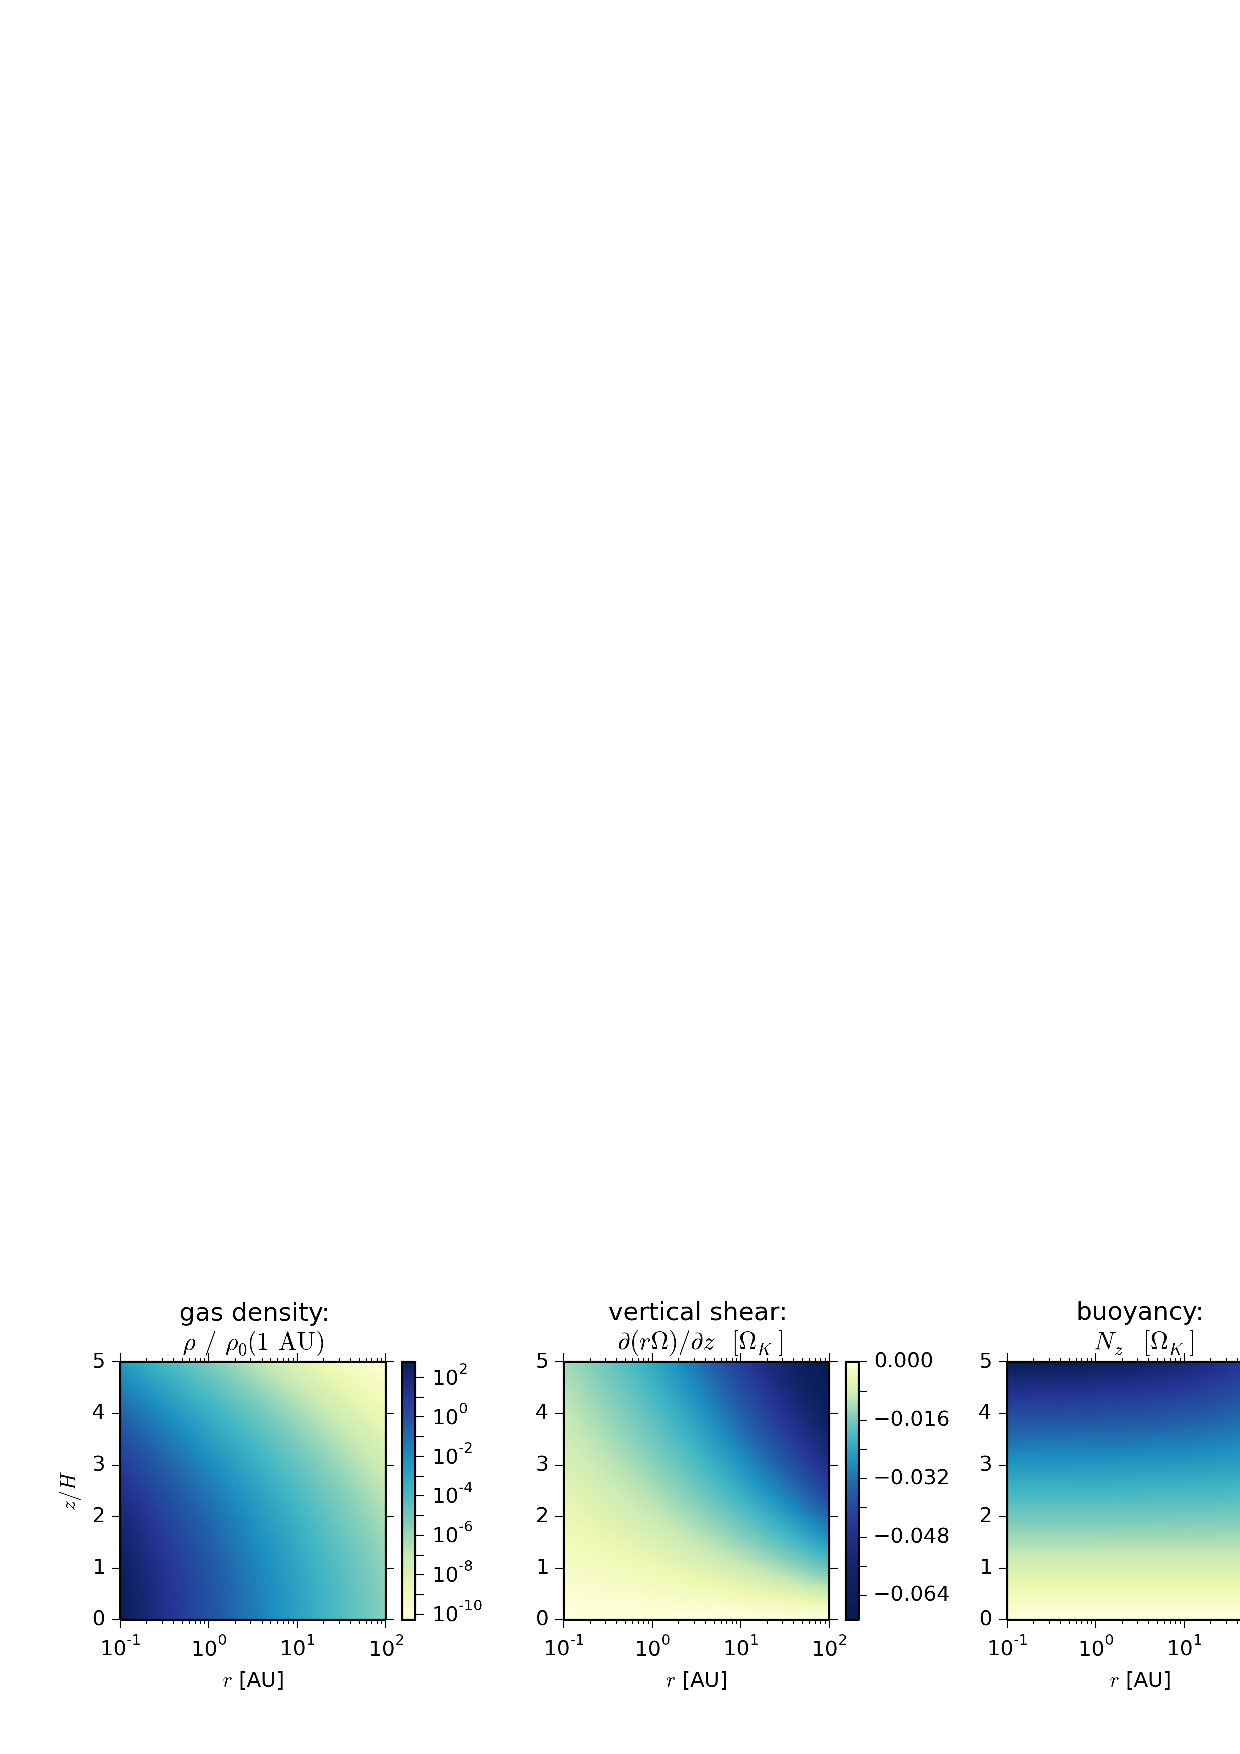
\includegraphics[width=\linewidth]{figures/rhoshearNz}
  \caption{The radial and vertical structure of a `minimum mass' PPD model showing gas density (left, relative to the midplane density at 1 AU), vertical shear rate (middle) and
    buoyancy frequency (right).
    \label{eqm_structure} 
  }
\end{figure*}

For a thin disk ($h\ll 1$), the vertical shear rate varies with height, $z$, from the midplane as 
\begin{align}\label{vshear_thin}
  r \frac{\p \Omega }{\p z} \simeq  h q \OmK \left(\frac{z}{2 H}\right),
\end{align}
where $H=hr$ is the characteristic disk scale height. 

This destabilizing shear competes with the stabilizing vertical
buoyancy frequency, $N_z$.  In a thin disk,     
\begin{align}\label{nz_thin}
  N_z^2 \simeq \left(\frac{\gamma-1}{\gamma}\right) \left(\frac{z}{H}\right)^2
  \OmK^2.  
\end{align}
Fig. \ref{eqm_structure} maps the vertical shear rate and buoyancy
frequency (as well as the gas density) 
in a fiducial PPD model, see \S\ref{toy_relax} for details. 

Vertical shear is 
generally weak compared to buoyancy, suggesting stability. In fact, 
without any cooling, the Solberg-Hoiland criteria %\citep{tassoul78}  Tassoul cited in S-H section is enough
confirms that vertical buoyancy is strong
enough to ensure (axisymmetric) stability, see \S\ref{solberg}.  With radiative cooling, 
thermal fluctuations decay which, combined with pressure equilibration, reduces the effective buoyancy.

How short must $t_c$ be for vertical shear to prevail?  We start with 
 the Richardson number $\mathrm{Ri} = N_z^2/(r\p_z\Omega)^2$, a 
ratio of buoyant to shear energies.  Though not precisely applicable to our problem,
non-rotating shear flows are stable if $\mathrm{Ri} > 1/4$ (\citealp{chandrasekhar61}, 
also see \citealp{ys02, lee10} for applications to thin dust layers in PPDs).
Following \cite{urpin03} and \cite{townsend58},  we reduce the buoyant energy by the 
ratio of cooling to forcing timescales, $t_c |r \p_z\Omega| \leq 1$ (with no reduction in buoyant energy 
expected when this inequality fails).  With this reduction, the Richardson-like criterion for 
shear instability becomes  \citep{urpin03}
\begin{align}\label{bcrit_est}
  t_c \lesssim \frac{\left|r\p\Omega/\p z\right|} {N_z^2}.
\end{align}
If we interpret Eq.\ \ref{bcrit_est} as a local criterion, then we see that 
the maximum cooling time which permits instability decreases with height as $1/|z|$;  
the stabilizing effect of vertical buoyancy increases more rapidly away from
the midplane than the destabilizing effect of vertical shear.  
This finding is relevant to the radiative damping of so called `surface 
modes', which we consider in \S\ref{numerical}.

We are more interested, however, in the global instability criterion for disturbances at all heights.
Our key result 
is the cooling requirement 
\begin{align}\label{prelim_bcrit}
  t_c <  &\frac{h |q| }{\gamma - 1}\OmK^{-1}
\end{align}   
for VSI growth that we derive in \S\ref{iso_vsi_beta_crit}.  We can simply 
(but non-rigorously) obtain Eq. \ref{prelim_bcrit}
by evaluating  Eq. \ref{bcrit_est} at $|z|=\gamma H/2$. 
 
\begin{figure}
  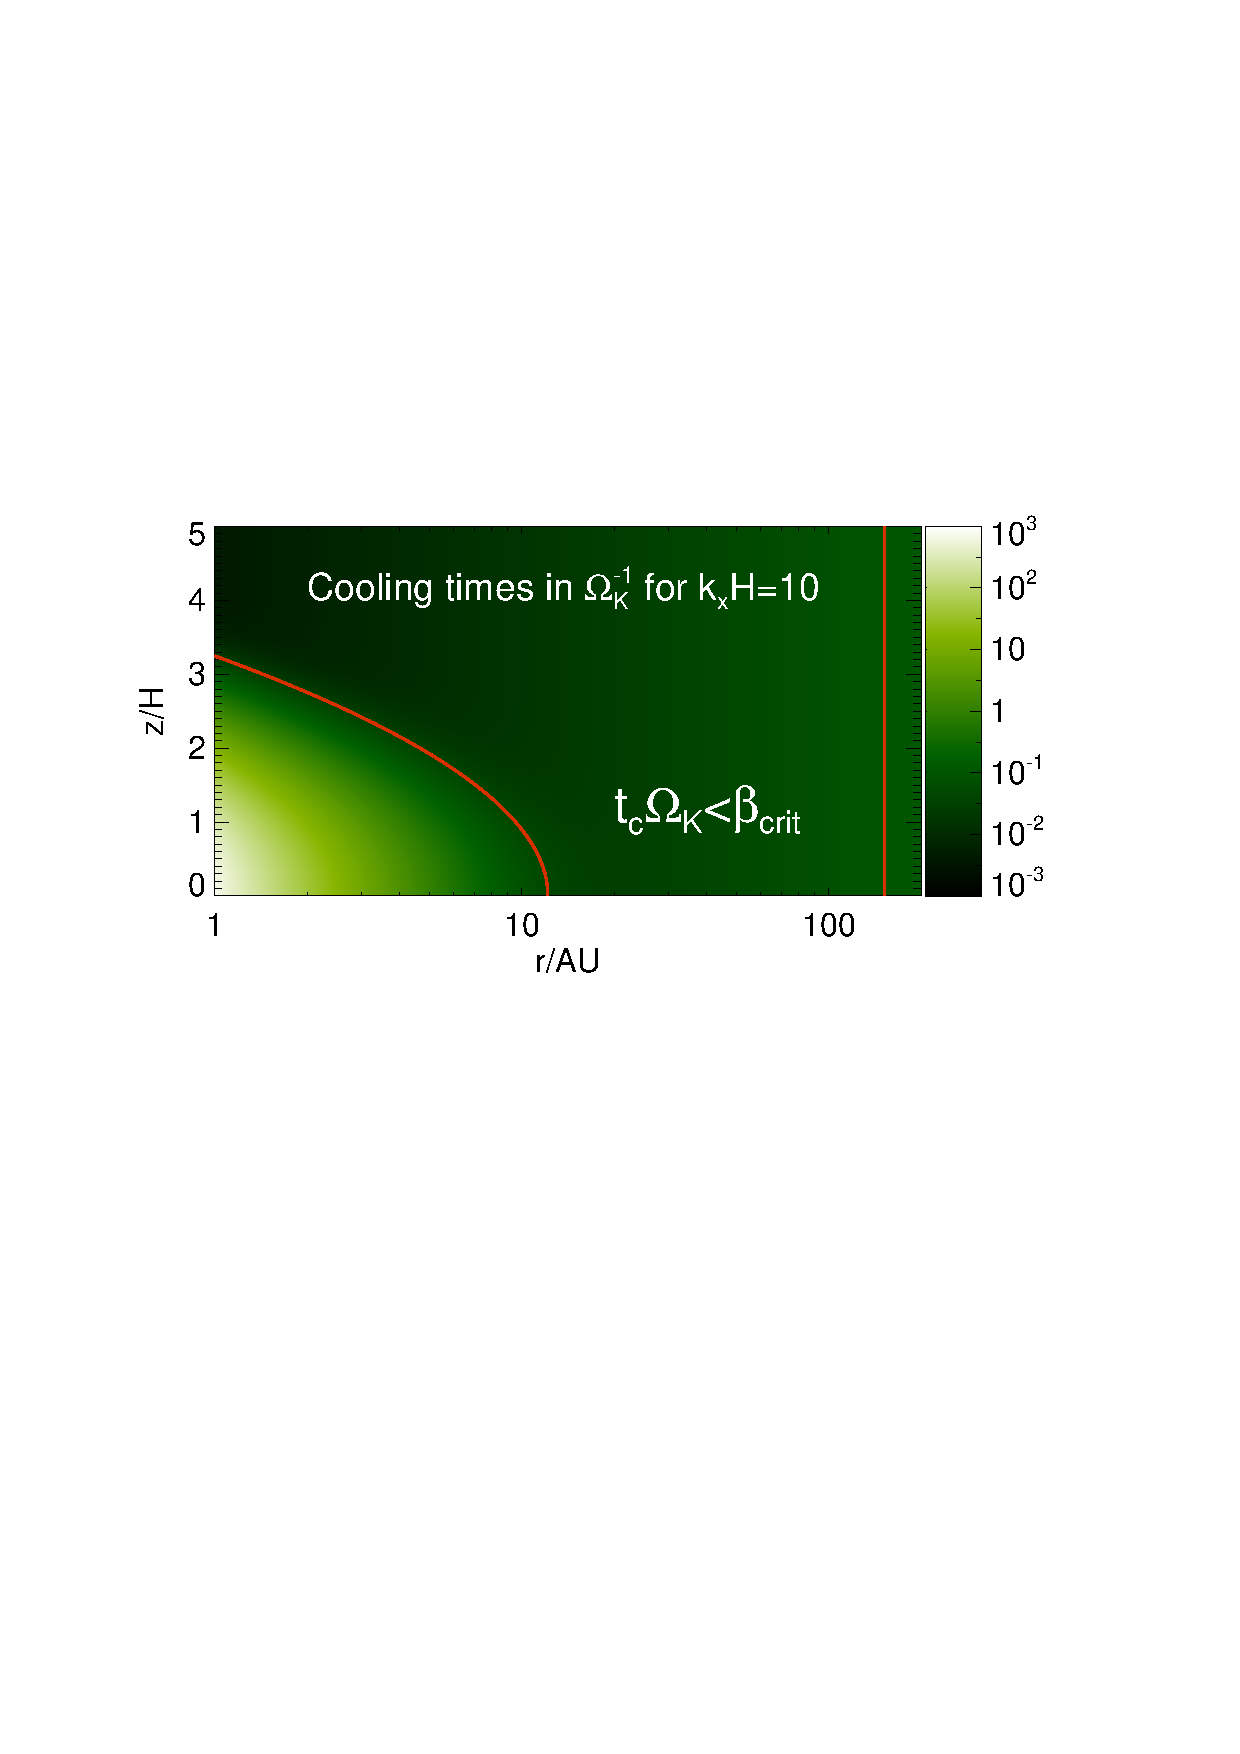
\includegraphics[width=\linewidth,clip=true,trim=0cm 1.7cm 0cm
  0.73cm]{figures/bcrit_mmsn2d_kx10}
  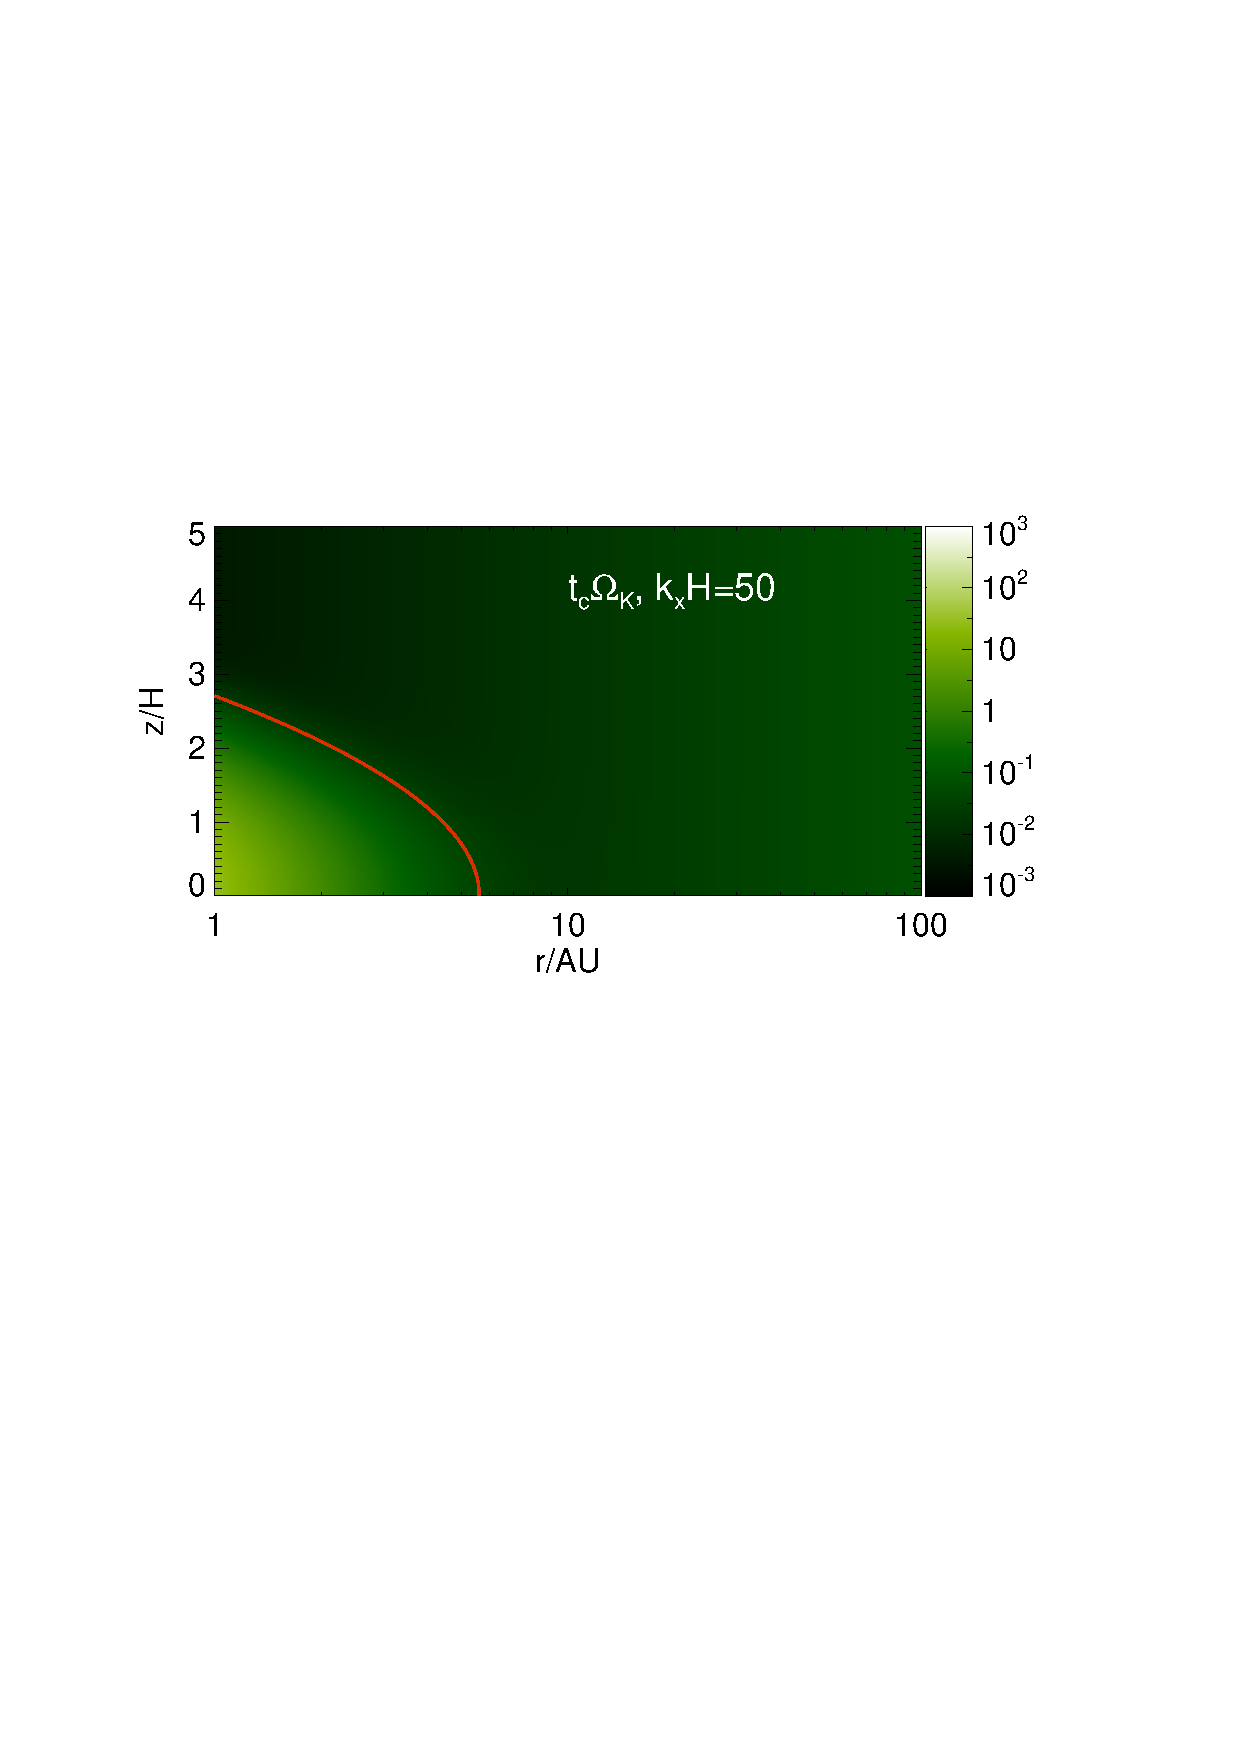
\includegraphics[width=\linewidth,clip=true,trim=0cm 0.46cm 0cm
  0.73cm]{figures/bcrit_mmsn2d_kx50}
  \caption{Estimate of the thermal timescale $t_c$  in a fiducial 
    PPD model, the Minimum Mass Solar Nebula. Here, $\beta_\mathrm{crit}=h|q|/(\gamma-1)$  
    is a maximum dimensionless cooling timescale below which the VSI
    is expected to operate effectively. This corresponds to   
    the region bounded by the red lines. 
    \label{bcrit_mmsn2d} 
  }
\end{figure}

We now consider whether, and where, thermal timescales in realistic PPDs
are short enough to support VSI growth.  Fig. \ref{bcrit_mmsn2d} plots the
 thermal timescales in our fiducial PPD model, see \S\ref{toy_relax} for details.
 The regions between the red lines satisfy the cooling requirement of Eq.\ \ref{prelim_bcrit}.
 Even without a detailed analysis we can expect VSI growth between $\sim 10$ -- 150AU.
 The inner disk is complicated by the fact that the optically thick
 midplane has longer cooling times.  
 Thus the cooling criterion fails in the midplane but is satisfied
 above.  This case requires the  
 more detailed analysis of \S\ref{application}.
 
  Fig. \ref{bcrit_mmsn2d} also compares two different radial wavenumbers, 
  $k_x = 10/H$ and $50/H$.  In the inner disk, the higher wavenumber
  mode cools faster, due to radiative diffusion. 
  Thus in the inner disk, shorter wavelength VSI modes are more likely
  to grow. In the outer disk, the cooling time is the  
  same for different $k_x$ and $z$, because optically thin cooling is
  independent of both lengthscale and density. 
  Thus the outer barrier to growth, beyond $\sim 150$ AU in this
  model, is independent of  wavelength.  
This example highlights the fact that optically thin cooling sets a
lower limit to the cooling time; a fact that is sometimes obscured
when  
the radiative diffusion approximation is made at the outset.   
 
 
% Since cooling by radiative diffusion depends on a perturbation's lengthscale, we
% plot $t_c$ for two values of the radial wavenumber,  $k_x$,  the relevant 
% component for VSI modes that are radially narrow.  The red line
%marks the boundary implied by Eq. \ref{prelim_bcrit}.  We caution that 
% Eq. \ref{prelim_bcrit} applies when $t_c$ is vertically uniform.  This section is 
% aimed at basic insights; while more realistic spatial variations in
% $t_c$ are considered in \S\ref{application}. 
% %analyzes the VSI with realistic spatial variations in.
% 
% Due to the smaller values of $t_c$ in the outer disk, we generally expect the VSI to 
% operate outside $\sim 10$ AU.  This conclusion changes however, if
% the dust opacity is reduced,  
%slowing down cooling, as we show in \S\ref{application}. % (e.g.\ Fig.\
%% \ref{mmsn_bcrit_bcool}). 
%In the inner disk, thermal times are long in the midplane, but short at higher altitutdes. 
%Again, this structure necessitates the more detailed analyses that follow.  Nevertheless, we can already 
%see that due to radiative diffusion higher wavenumbers can cool more rapidly.  Thus smaller scale disturbances 
%may trigger VSI at smaller disk radii. 
%
%On the other hand, one cannot obtain arbitrarily short cooling times
%by invoking arbitrarily small scales (cf. \citealt{urpin03}, 
%\citetalias{barker15}), because very small wavelengths are in the
%optically thin cooling regime,  where cooling is independent of
%lengthscale. Furthermore, 
%%while we do not include viscosity in our
%%idealized disk models, in reality 
%small-scale perturbations will be 
%prone to viscous damping, including the effective viscosity from turbulent motions.
%While our linear, inviscid calculations do not address this issue directly, we expect that 
%shorter wavelength modes will drive weaker non-linear (and non-axisymmetric) transport. 
%
%% However, we cannot and do not find that VSI will always be relevant for
%% sufficiently small perturbations because \begin{inparaenum}[(i)] \item very small wavelengths are in the optically 
%% thin cooling regime,  where cooling is independent of lengthscale;
%% and \item small scale perturbations 
%% are more prone to viscous damping, and should drive weaker transport.
%% \end{inparaenum} 
%
%We now proceed with our detailed analysis of the VSI to arrive
%at Eq. \ref{prelim_bcrit} and verify it numerically. The interested 
%reader may jump to \S\ref{application} for the application of our
%results to PPDs.     

\section{Governing equations and disk models}\label{setup}
We consider  an inviscid, non-self-gravitating three-dimensional (3D)
disk orbiting a central star of mass $M_*$. We adopt cylindrical
co-ordinates $(r,\phi, z)$ centered on the star to describe the global
disk. The governing fluid equations are
\begin{align}
  &\frac{\p\rho}{\p t} + \nabla\cdot{\left(\rho\bm{v}\right)} = 0,\\
  &\frac{\p\bm{v}}{\p t} + \bm{v}\cdot\nabla\bm{v} =
  -\frac{1}{\rho}\nabla P - \nabla\Phi_*,\\
  &\frac{\p P}{\p t} + \bm{v}\cdot\nabla P  = - \gamma P
  \nabla\cdot\bm{v} - \frac{\rho}{t_c}\left(\frac{P}{\rho} -
    \left.\frac{P}{\rho}\right|_{t=0}\right), \label{full_energy}
\end{align}
where $\rho$ is the mass density, $\bm{v}$ is the velocity field (the
rotation frequency being $\Omega=v_\phi/r$), $P$
is the pressure, $\gamma$ is the constant adiabatic index, and $\Phi_*
= -GM_*(r^2 + z^2)^{-1/2}$ is the gravitational potential of the
central star and $G$ is the gravitational constant. 
In the energy equation (Eq. \ref{full_energy}) we have
included a thermal relaxation term which restores the disk temperature
$T\propto P/\rho$ to its initial value on a characteristic timescale
$t_c=\beta\Omega_k^{-1}$ where $\beta$ is a dimensionless coefficient
and $\Omega_k=\sqrt{GM_*/r^3}$ is the Keplerian frequency. 

\subsection{Baroclinic disk equilibria}\label{eqm}
The equilibrium disk is steady and axisymmetric with density,
pressure and rotation profiles $\rho(r,z)$, $P(r,z)$ and
$\Omega(r,z)$, respectively. The equilibrium disk satisfies
\begin{align}
  0 &= \frac{1}{\rho}\frac{\p P}{\p z} + \frac{\p \Phi_*}{\p z},\label{vert_equilibrium}\\
  r\Omega^2&= \frac{1}{\rho}\frac{\p P}{\p r} + \frac{\p \Phi_*}{\p
    r}.\label{hori_equilibrium} 
\end{align} 
%where $\Phi_* = -GM_*(r^2 + z^2)^{-1/2}$ is the gravitational
%potential of the central star.
We examine disks with power-law profiles for the midplane density
$\rho_0(r)\equiv\rho(r,0)$: 
\begin{align}
  \rho_0(r) = \rho_{00}\left(\frac{r}{r_0}\right)^p,
\end{align}
where $\rho_{00}$ is the midplane density at the fiducial radius
$r=r_0$ and $p$ is the power-law index. The equilibrium pressure $P$
and density $\rho$ are related by 
\begin{align}
  P(r,z) &= 
  \frac{c_{s0}^2(r)}{\Gamma}\rho_0(r)^{1-\Gamma}\rho^\Gamma(r,z),\notag\\
  & \equiv K(r)\rho^{\Gamma}(r,z). \label{eqm_press}
\end{align}
where the polytropic index $\Gamma$ is a parameter and 
the midplane sound-speed $c_{s0}(r)$ is taken to be another power-law: 
\begin{align}
  c_{s0}^2(r)=c_{s00}^2\left(\frac{r}{r_0}\right)^q, 
\end{align}
where $c_{s00}\equiv c_{s0}(r_0)$  and $q$ is the power-law index for
the midplane temperature. We define
\begin{align}
  \epsilon(r) \equiv \frac{c_{s0}(r)}{v_k(r)} \equiv
  \frac{H_\mathrm{iso}}{r} 
\end{align}
to parametrize the magnitude of the sound-speed, where
$v_k=r\Omega_k$ is the Keplerian azimuthal velocity and
$H_\mathrm{iso}$ is a characteristic scale-height.  Thus, $\epsilon$
is also the characteristic disk aspect-ratio.  

The global sound-speed $c_s(r,z)$ is given by
\begin{align}
  c_s^2\equiv \frac{dP}{d\rho} =
  c_{s0}^2(r)\left(\frac{\rho}{\rho_0}\right)^{\Gamma-1} = \frac{\Gamma P}{\rho}. 
\end{align}
For discussion purposes it is useful to define the vertical buoyancy frequency $N_z$ via
\begin{align}
  N_z^2 = c_s^2 \left(\frac{\gamma -
      \Gamma}{\gamma}\right)\left(\frac{\p\ln\rho}{\p z}\right)^2,   
\end{align}
where $\gamma$ is the constant adiabatic index. We are interested in
neutrally or sub-adiabatically stratified 
disks with $\Gamma\leq \gamma$ so that $N_z^2\geq0$.  

The explicit expression for the density field for
$\Gamma\neq1$ is given  by
\begin{align}\label{eqm_dens}
  &\left(\frac{\rho}{\rho_0}\right)^{\Gamma-1} = 1 +
  \frac{\left(\Gamma-1\right)}{\epsilon^2}\left(\frac{1}{\sqrt{1+z^2/r^2}}-1\right),
\end{align}
Note that for $\Gamma\neq1$ the disk has a surface $z=H(r)$ such that
$\rho(r,H)=0$. If we parametrize
\begin{align}
  H(r)\equiv h r,
\end{align}
then the imposed sound-speed and disk thickness are related by 
\begin{align}
  h^2(r) = \left[1-\frac{\epsilon^2(r)}{\Gamma-1}\right]^{-2}-1. 
\end{align}
Similarly, the equilibrium rotation is 
\begin{align}\label{eqm_rot}
  \frac{\Omega^2(r,z)}{\Omega_k^2(r)}=1 +
  \left(p+\frac{s}{\Gamma}\right)\epsilon^2(r) 
  +\frac{s}{\Gamma} \left(1-\frac{1}{\sqrt{1+z^2/r^2}}\right), 
\end{align}
where $s\equiv q+p(1-\Gamma)$. We also define the radial shear rate  
\begin{align}
  S(r,z) \equiv r\frac{\p\Omega}{\p r},  
\end{align}
and the square of the epicyclic frequency $\kappa$ 
\begin{align}
  \kappa^2(r,z) \equiv 2\Omega(2\Omega + S). 
\end{align}

Note that the disk is in general baroclinic with $\Omega =
\Omega(r,z)$. This is explicit from Eq. \ref{eqm_rot}, but is also
implied by Eq. \ref{vert_equilibrium}---\ref{hori_equilibrium} and 
Eq. \ref{eqm_press},  
\begin{align}
  r\frac{\p\Omega^2}{\p z} = - \rho^{\Gamma-1}\frac{\p\ln\rho}{\p
    z}\frac{dK}{dr}.\label{vertical_shear}
\end{align}

\subsubsection{Vertically isothermal disks}
For the special case $\Gamma=1$ the disk is isothermal in the
vertical direction. The equilibrium density $\rho(r,z)$ and rotation
$\Omega(r,z)$ is then 
\begin{align}
  \frac{\rho(r,z)}{\rho_0(r)} &=
  \exp{\left[\frac{1}{\epsilon^2}\left(\frac{1}{\sqrt{1+z^2/r^2}}-1\right)\right]}\\    
  \frac{\Omega^2(r,z)}{\Omega_k^2(r)}& =1+ (p+q)\epsilon^2(r) + q\left(1 -
    \frac{1}{\sqrt{1+z^2/r^2}}\right),\label{vertiso_eqm}
\end{align}
which may be obtained from Eq. \ref{eqm_dens} and Eq. \ref{eqm_rot} by
taking the limit $\Gamma\to 1$. We will, in fact, primarily focus on
vertically isothermal disks for simplicity. 


\subsection{Stability condition against axisymmetric adiabatic
  perturbations}\label{solberg}
A rotating flow is stable against axisymmetric adiabatic perturbations
if both Solberg-Hoiland criteria  are satisfied:
\begin{align}
  \kappa^2 - \frac{1}{\rho c_p}\nabla P \cdot \nabla S &> 0,\\
  -\frac{\p P}{\p z}\left(\frac{\p j^2}{\p r}\frac{\p S}{ \p z} -
    \frac{\p j^2}{\p z}\frac{\p S}{\p r} \right)&>0. \label{second_SH} 
\end{align}
\citep{tassoul78}, where $S = c_p\ln{P^{1/\gamma}/\rho}$ is the
specific entropy, $c_p$ is the heat capacity at constant
pressure, and $j\equiv r^2\Omega$ is the
specific angular momentum.   

For rotationally-supported, thin disks, pressure gradients are small 
compared to rotation, so the first criterion is generally
satisfied. Thus, to assess stability, we consider the second
criterion. For our disk models,
\begin{align}
  &\frac{\p S}{\p r} = c_p\left[\frac{s}{\gamma r} +
    \left(\frac{\Gamma}{\gamma}-1\right)\frac{\p \ln{\rho}}{\p
       r}\right],\\
  &\frac{\p S}{\p z} = c_p
  \left(\frac{\Gamma}{\gamma}-1\right)\frac{\p \ln{\rho}}{\p z}. 
\end{align} 
Without loss of generality, we evaluate Eq. \ref{second_SH} in $z>0$
where $\p_zP<0$. Here we approximate $\p_r j^2\simeq r^3\Omega_k^2$ but
use Eq. \ref{vertical_shear} for $\p_zj^2$. Then 
\begin{align}\label{solberg2}
  % \gamma - \Gamma > \frac{s\epsilon^2}{\Gamma}
  % \left(\frac{\rho}{\rho_0}\right)^{\Gamma-1} \left[s
  %   -\left(\gamma-\Gamma\right)\frac{\p\ln{\rho}}{\p\ln{r}} \right]. 
  \gamma - \Gamma > \frac{\epsilon^2}{\Gamma}
  \left(\frac{\rho}{\rho_0}\right)^{\Gamma-1} \left[s^2
    -s\left(\gamma-\Gamma\right)\frac{\p\ln{\rho}}{\p\ln{r}} \right]. 
\end{align} 
For typical model parameters the right hand side is
$O(\epsilon^2)$. Hence, instability in the adiabatic limit 
requires $\gamma < \Gamma + O(\epsilon^2)$. Since we consider
$\epsilon\ll1$, this implies the equilibrium disk must have a small
entropy gradient in order to be unstable to axisymmetric adiabatic
perturbations. 

\section{Linear problem}\label{linear}
We consider axisymmetric perturbations to the above equilibria in the
form 
\begin{align}
  \rho \to \rho(z) + \delta\rho(r,z)\exp{\left( - \ii\sigma
      t\right)},    
\end{align}
and similarly for other fluid variables, where $\sigma = \omega + \ii
\nu$ is a (generally) complex frequency, with $\omega$ and $\nu$ being
the real frequency and growth rate, respectively.

The linearized fluid equations in cylindrical co-ordinates are  
\begin{align}
  \ii\sigma\delta\rho &= \frac{\rho}{r}\frac{\p}{\p r}\left(r\delta v_r\right) + \frac{\p}{\p
    z}\left(\rho\delta v_z\right)  + \hat{g}_c\frac{\p\rho}{\p r}\delta v_r,\\
  \ii\sigma\delta v_r &= \frac{1}{\rho}\frac{\p\delta P}{\p r} - 2\Omega
  \delta v_\phi - \hat{g}_c\frac{\delta\rho}{\rho^2}\frac{\p P}{\p r},\\ 
  \ii\sigma\delta v_\phi  &= \frac{\kappa^2}{2\Omega}\delta v_r +
  r\frac{\p\Omega}{\p z}\delta v_z,\\
  \ii \sigma\delta v_z &= \frac{1}{\rho}\frac{\p\delta P}{\p z} -
  \frac{\delta \rho}{\rho^2}\frac{\p P}{\p z},\\
  \ii\sigma\delta P &=\frac{\p P}{\p z}\delta v_z + \gamma P
  \left[\frac{1}{r}\frac{\p}{\p r}\left(r\delta v_r\right) + \frac{\p
      \delta v_z}{\p z}\right]\notag \\
  &+ \frac{1}{t_c}\left(\delta P -  
    \frac{P}{\rho}\delta\rho\right) + \hat{g}_c \frac{\p P}{\p r}\delta v_r,\label{full_energy1}
\end{align}
where the coefficients $\hat{g}_c=1$ are inserted to label terms
associated with the background radial disk structure. 

\subsection{Radially-local approximation}  
We consider perturbations with small radial lengthscales 
so that we can ignore the radial variations in the background
structure and radial gradients. We thus evaluate all coefficients in
the above equations at the fiducial radius $r=r_0$. However, the full
vertical dependence of the coefficients are retained. Then we can
assume perturbations have spatial dependence in the form
\begin{align}
  \delta \rho(r,z) \to \delta\rho(z)\exp{\ii k_r r},
\end{align}
and we assume $|k_rr|\gg1$ so that curvature terms can also be
ignored.       

In order to emphasize the radially-local approximation, we
introduce the local Cartesian co-ordinate $(x,y,z)$ corresponding to
the the local $(r,\phi,z)$ directions, respectively. Then writing
$\delta P /\rho \equiv W$ and $c_s^2\delta\rho/\rho\equiv Q$, the
linearized system of equations are 
\begin{align}
  \ii\sigma \frac{Q}{c_s^2}  &=  \ii k_x \delta v_x + \frac{d\dd
    v_z}{dz} + \frac{\p\ln{\rho}}{\p z}\delta v_z + \hat{g}_c
  \frac{\p\ln{\rho}}{\p r} \delta v_x,\label{lin_mass}\\
  \ii\sigma \delta v_x  &= \ii k_x W - 2\Omega\delta v_y -
  \hat{g}_c\frac{1}{\rho}\frac{\p P}{\p r}\frac{Q}{c_s^2}\label{lin_vx}\\
   \ii \sigma\delta v_y &= r\frac{\p \Omega}{\p z}\delta v_z +
  \frac{\kappa^2}{2\Omega}\delta v_x, \label{lin_vy}\\
   \ii\sigma\delta v_z &= \frac{dW}{dz} +
  \frac{\p\ln{\rho}}{\p z}\left(W-Q\right), \label{lin_vz}\\
  \ii \sigma W &= c_s^2\frac{\p\ln{\rho}}{\p z}\delta v_z +
  c_s^2\frac{\gamma}{\Gamma} \left(\ii k_x\delta v_x + \frac{d\delta
      v_z}{dz}\right) \notag\\
  &+ \frac{1}{t_c}\left(W - \frac{Q}{\Gamma}\right) +
  \hat{g}_c\frac{1}{\rho}\frac{\p P}{\p r}\delta v_x.\label{lin_energy}
  % -&\ii\sigma W + \frac{1}{t_c}\left(W-\frac{Q}{\Gamma}\right) = -\ii\sigma\frac{\gamma}{\Gamma} Q +
  % c_s^2\frac{d\ln{\rho}}{dz}\left(\frac{\gamma}{\Gamma}-1\right)\delta v_z.\label{lin_energy}
\end{align}
It is understood that the quantities $\rho,\,c_s^2,\,\Omega,\kappa,\, 
\p_z\Omega,\, \p_r\ln{\rho} $ and $ \p_r P$ are evaluated at $r=r_0$.   
Eq. \ref{lin_mass}---\ref{lin_energy} will form the basis of our numerical
study, but for analytical discussion
we will make further simplifications. 










% We are interested in the axisymmetric stability of the above system,
% on radial length-scales much smaller than the local radius $r$, but
% may be global in the vertical direction. As such, we work within the
% framework of the \emph{vertically global shearing 
%   box} (VGSB) developed by \cite{mcnally14}. In this approximation
% one sets up a local Cartesian co-ordinate  system $(x,y,z)$ centered
% on a fiducial point $(r,\phi,z)=(r_0,\phi_0,0)$ in the global disk, with $\phi_0(t) =
% \Omega(r_0,0)t$. The local $x,y,z$ axis correspond to the
% global radial, azimuthal and vertical directions.  

% In this shearing box the equilibrium density, pressure and
% sound-speed are assumed to depend only on $z$, by evaluating these
% quantities at $r=r_0$ in the global disk. The background rotation
% $\Omega$ is approximated by a linear shear in $x$, but left unaltered
% in $z$. However, the vertical shear $\p_z\Omega$ is also assumed to
% only depend on $z$.     

% The axisymmetric VGSB equations read 
% \begin{align}
%   & \frac{\p\rho}{\p t} + \frac{\p}{\p x}\left(\rho v_x\right) +
%   \frac{\p}{\p z}\left(\rho v_z\right)=0,\\
%   & \frac{\p\bm{v}}{\p t} + \bm{v}\cdot\nabla\bm{v} +
%   v_zr_0\frac{d\Omega_0}{dz} \hat{\bm{y}} = - 
%   2\Omega_0\hat{\bm{z}}\times\bm{v} - S_0v_x\hat{\bm{y}} \notag\\ 
%   &\phantom{\frac{\p\bm{v}}{\p t} + \bm{v}\cdot\nabla\bm{v} +
%     v_zr_0\frac{d\Omega_0}{dz} \hat{\bm{y}}=}-\frac{1}{\rho}\nabla P - \frac{\p\Phi_0}{\p z}\hat{\bm{z}},\\
%   & \frac{\p P}{\p t} + \bm{v}\cdot\nabla P = -\gamma P
%   \nabla\cdot\bm{v} -
%   \frac{\rho}{t_c}\left(\frac{P}{\rho}-\left.\frac{P}{\rho}\right|_{t=0}\right), \label{energy_eq}
% \end{align}
% where $\bm{v}$ is the velocity field relative to the bulk flow
% (i.e. $\bm{v}=\bm{0}$ in equilibrium),  
% subscript $0$ indicates evaluation at $r=r_0$. In the energy equation 
% we have added a thermal relaxation term with timescale
% $t_c=\beta\Omega_k^{-1}$ with $\beta$  being a dimensionless input
% parameter.  

% \subsection{Linearization}
% We perturb the system such that
%  For clarity we drop the subscript $0$ on the
% frequencies and shear rates below.  

% We can eliminate the perturbed velocities between the linearized
% equations to obtain a pair or ordinary differential equations
% for $W,Q$ as
% \begin{align}
%   &\frac{\sigma^2}{c_s^2}Q + \frac{\sigma^2k_x^2}{D}W \notag\\ 
%   &=\left(\frac{\ii
%     k_x r}{D}\frac{d\Omega^2}{dz} -
%   \frac{d\ln{\rho}}{dz}\right)\left[\frac{dW}{dz} +
%   \frac{d\ln{\rho}}{dz}\left(W-Q\right)\right] \notag\\
% &- \frac{d^2W}{dz^2} - \frac{d\ln{\rho}}{dz}\left(\frac{dW}{dz} -
%   \frac{dQ}{dz}\right) - \frac{d^2\ln{\rho}}{dz^2}\left(W-Q\right),\label{ode_w}\\
% &\sigma^2W - \frac{\gamma}{\Gamma}\sigma^2 Q +
% \frac{\ii\sigma}{t_c}\left(W-\frac{Q}{\Gamma}\right)\notag\\
% &=c_s^2\frac{d\ln{\rho}}{dz}\left(\frac{\gamma}{\Gamma} - 1\right) 
% \left[\frac{dW}{dz} + \frac{d\ln{\rho}}{dz}\left(W-Q\right)\right],\label{ode_Q} 
% \end{align}
% where
% \begin{align}
%   D \equiv \kappa^2 - \sigma^2.
% \end{align}




\section{Vertically isothermal disks with 
  isothermal perturbations}
The linear problem simplifies considerably for the case
$\Gamma=\gamma=1$. Then 
\begin{align}
  Q=W. 
\end{align}

Inserting this into Eq. \ref{ode_w} gives a single equation for the linear stability
problem for isothermal perturbations in a vertically isothermal disk, 
\begin{align}\label{iso_ode}
  \frac{d^2W}{dz^2} + \left(\frac{d\ln{\rho}}{dz} - \frac{\ii k_x
      r}{D}\frac{d\Omega^2}{dz}\right) \frac{dW}{dz} +
  \sigma^2\left(\frac{1}{c_s^2} + \frac{k_x^2}{D}\right)W=0, 
\end{align} 
subject to appropriate boundary conditions. We remark that Eq
.\ref{iso_ode} is also applicable for    
$\gamma=\Gamma\neq 1$ in the limit $t_c\to\infty$ (i.e. adiabatic
disks with adiabatic vertical stratification), since in that case  
$Q\simeq W$ as well. 


\subsection{Neccessity of vertical shear for instability}\label{integral_relation}
We can establish a neccessary condition for instability with the
following assumptions:

\begin{enumerate}
\item We consider eigenvalues such that
  $|\sigma^2|\ll \kappa^2$. Then we can replace $D=\kappa^2 -\sigma^2\to
  \kappa^2$. The problem simplifies because the eigenvalue now only
  appears in the last term in Eq. \ref{iso_ode}. 
\item We are mainly interested in the effect of vertical shear, i.e. $q\neq
0$. This is already captured explicitly in Eq. \ref{iso_ode} through
the factor $d\Omega^2/dz$. We 
therefore simplify further by ignoring the vertical dependence of
$\kappa^2$. For clarity, we will replace  $\kappa^2$ with $\Omega_k^2$.  
\end{enumerate}

With these approximations we can re-write the governing equation as
\begin{align}\label{iso_ode1}
  &\frac{d}{dz}\left(\rho e^{-\ii k_x r
      \Omega^2/\Omega_k^2}\frac{dW}{dz}\right) +
  \sigma^2\left(\frac{1}{c_s^2}+\frac{k_x^2}{\Omega_k^2}\right) \rho W e^{-\ii k_x r
    \Omega^2/\Omega_k^2} \notag\\
  &=0.
\end{align}
Next, we multiply Eq. \ref{iso_ode1} by $W^{*}\exp{\left(\ii k_x r
    \Omega^2/\Omega_k\right)}$, integrate 
vertically and assume boundary terms vanish to obtain
\begin{align}\label{neccessary_cond}
   &\sigma^2\left(\frac{1}{c_s^2}+\frac{k_x^2}{\Omega_k^2}\right)\int_{-\infty}^{\infty}\rho|W|^2dz \notag\\
  &=\int_{-\infty}^{\infty}\rho\left|\frac{dW}{dz}\right|^2dz 
  +\frac{\ii k_x r}{\Omega_k^2}\int_{-\infty}^{\infty}\rho\frac{d\Omega^2}{dz}W^*\frac{dW}{dz}dz. 
\end{align}
It follows that for instability ($\imag\sigma>0$), it is neccessary to
have $d\Omega^2/dz\neq 0$, i.e. vertical shear.  


\subsection{Thin-disk limit}
The full expressions for the equilibrium density and vertical shear
depends on $z$ in a non-trivial manner. Thus, to simplify the problem 
we consider thin-disks ($\epsilon\ll1$), 
so we may expand the background density and vertical shear in powers
of $z/r$. To lowest order we obtain
\begin{align}
  &\rho(z) \simeq \rho_{00} \exp{\left(-\frac{z^2}{2\Hiso^2}\right)},\label{thin_dens}\\
  &\frac{d\Omega^2}{dz} \simeq \frac{q\Omega_k^2z}{r^2}. \label{thin_vshear}
\end{align}


With this approximation and those in \S\ref{integral_relation}, the
governing equation becomes
\begin{align}\label{iso_ode3}
  \frac{d^2W}{d\hat{z}^2} - \left(1 + \ii q\epsilon
    \hat{k}\right)\hat{z}\frac{dW}{d\hat{z}} +
  \left(\frac{\sigma}{\Omega_k}\right)^2\left(1+\hat{k}^2\right)W = 
  0, 
\end{align}
where we have introduced the dimensionless vertical co-ordinate
$\hat{z} \equiv z/\Hiso$ and wavenumber $\hat{k} \equiv k_x \Hiso$. We 
remark that for large $|\hat{k}|$, Eq. \ref{iso_ode3} is the same as
that derived by \cite{nelson13}, although we have taken a different
route.  

In the thin-disk approximation the integral relation
Eq. \ref{neccessary_cond} becomes
\begin{align}\label{integral_relation_thin}
 & \left(\frac{\sigma}{\Omega_k}\right)^2\left(1+\hat{k}^2\right)
  \int_{-\infty}^{\infty}w|W|^2d\hat{z}  \notag\\ 
  & =\int_{-\infty}^{\infty}w\left|\frac{dW}{d\hat{z}}\right|^2d\hat{z}
  +\ii q \epsilon
  \hat{k}\int_{-\infty}^{\infty}w\hat{z}W^*\frac{dW}{d\hat{z}}d\hat{z}.    
\end{align}
where 
\begin{align}
  w(\hat{z}) \equiv \exp{\left(-\frac{\hat{z}^2}{2}\right)}.  
\end{align}


\subsection{Stability in the absence of vertical shear}
When $q=0$, Eq. \ref{iso_ode3} is
\begin{align}\label{hermite_ode}
  \frac{d}{d\hat{z}}\left[w(\hat{z})\frac{dW}{d\hat{z}}\right] + nW
  w(\hat{z}) =0, 
\end{align}
where we have defined a new eigenvalue
\begin{align}
  n \equiv \left(\frac{\sigma}{\Omega_k}\right)^2(1+\hat{k}^2). 
\end{align} 
Eq. \ref{iso_ode3} is Hermite's differential equation. If we impose
that the kinetic energy density remain bounded at infinity, then  
\begin{align}
  W \propto \He_n(\hat{z}),
\end{align}
and $n$ is a non-negative integer. This translates to a real
eigenfrequency $\sigma$ such that
\begin{align}
  \left|\frac{\sigma}{\Omega_k}\right| = \sqrt{n}
  \left(1+\hat{k}^2\right)^{-1/2}. 
\end{align}
Since we have assumed $|\sigma^2|\ll \kappa^2$, our analysis is only
valid for large wavenumbers such that $\hat{k}^2\gg 
n-1$. Physically, this corresponds to radial length-scales much
smaller than the local disk scale height. 

\subsection{Polynomial solutions with vertical shear}
We can seek power-series solution to Eq. \ref{iso_ode3},
\begin{align}
  W(\zhat) = \sum_{m=0}^\infty a_m\zhat^m. 
\end{align}
Then the coefficients must satisfy the recurrence relation
\begin{align}
  (m+2)(m+1)a_{m+2} +
  \left[n - m\left(1+\ii q h \hat{k}\right)\right] a_m = 0, 
\end{align}
where $n$ is not neccessarily an integer. Indeed, if we demand
a polynomial of degree $M$ as the solution, then the eigenfrequency
must satisfy
\begin{align}
\left(\frac{\sigma}{\Omega_k}\right)^2 = M\left(\frac{1+\ii q \epsilon
    \hat{k}}{1+\hat{k}^2}\right).
\end{align}
The eigenfrequency $\sigma$ is therefore complex. We are interested in
unstable modes for which $\imag{\sigma}$ is the growth rate and is
given by 
\begin{align}\label{simple_growth}
   \frac{\imag(\sigma)}{\Omega_k} =\sqrt{
   \frac{M}{2\left(1+\hat{k}^2\right)}\left(\sqrt{1+q^2\epsilon^2\hat{k}^2} - 
    1\right)}. 
\end{align}
For fixed $q$ and $\epsilon$, the growth rate vanishes for both
$\hat{k}^2\to0$ and $\hat{k}^2\to\infty$. The maximum growth rate
occurs at the optimum wavenumber $\hat{k}_\mathrm{opt}$
\begin{align}
  |\hat{k}_\mathrm{opt}| = \sqrt{\frac{2+|\epsilon q|}{|\epsilon q|}},
\end{align}
and
\begin{align}
\mathrm{max}\left[\imag(\sigma)\right] =\frac{\sqrt{M}|\epsilon
  q|}{2\sqrt{1+|\epsilon q|}}\Omega_k. 
\end{align}

% This expression can be simplified in the limit $|q|\ll 1$, 
%  \begin{align}\label{simple_growth}
%    \frac{\imag(\sigma)}{\Omega_k} = \pm \sqrt{M} 
%    \frac{q\epsilon\hat{k}}{2\sqrt{1+\hat{k}^2}} \quad\quad (|q|\ll 1), 
%  \end{align}
%  with $M$ being an integer. 


\subsection{Instability in the presence of weak vertical shear}
We can also investigate the destabilizing effect of vertical shear
without explicitly solving the full governing equation,
Eq. \ref{iso_ode3}. We first
consider a system with $q\equiv0$, for which the eigenfunctions are
Hermite polynomials and the real eigenfrequencies are known. We then
perturb this system by introducing a weak vertical shear ($|q|\ll1$)
and linearize the governing equation. This procedure is
\begin{align}   
  &q \to 0 + \delta q\\
  &W \to \He_n + \delta V \\
  &\sigma \to \sigma + \delta\sigma, 
\end{align}
where for this exercise we restore $\sigma$ as the eigenfrequency. 

Linearizing the integral relation in the thin-disk limit, Eq. \ref{integral_relation_thin}, and taking the
imaginary part, we have
\begin{align}
  \frac{2\sigma\imag(\delta\sigma)}{\Omega_k^2}
  \left(1+\hat{k}^2\right) \int_{-\infty}^{\infty} w(\zhat)
  \He_n^2(\hat{z}) d\hat{z} \notag\\
  = \delta q \epsilon \hat{k} 
  \int_{-\infty}^{\infty}
  w(\zhat)\hat{z}\He_n(\hat{z})\frac{d\He_n}{d\zhat} d\hat{z}
\end{align}
Recognizing $\hat{z} = \He_1$ and using $d\He_n/d\hat{z} = n
\He_{n-1}$ we have
 \begin{align}
   \frac{2\sigma\imag(\delta\sigma)}{\Omega_k^2}
   \left(1+\hat{k}^2\right) \int_{-\infty}^{\infty} w(\zhat)
   \He_n^2(\hat{z}) d\hat{z} \notag\\
   =\delta q \epsilon \hat{k} 
   \int_{-\infty}^{\infty}
   w(\zhat)\He_1(\hat{z})\He_n(\hat{z})n\He_{n-1}(\hat{z})d\hat{z}. 
 \end{align}

Finally, we evaluate the integrals using the results
\begin{align}
  \int_{-\infty}^{\infty}
  w(\xi) \He_k(\xi)\He_l(\xi) d\xi = \sqrt{2\pi}k!\delta_{kl}, 
\end{align}
and
\begin{align}
  &\int_{-\infty}^{\infty}
  w(\xi) \He_m(\xi)\He_k(\xi)\He_l(\xi) d\xi\notag\\& =
  \frac{\sqrt{2\pi}m!k!l!}{(j-m)!(j-k)!(j-l)!}, 
\end{align}
where $j = (m+k+l)/2$. We then obtain

 \begin{align}
  \frac{2\sigma\imag(\delta\sigma)}{\Omega_k^2}
  \left(1+\hat{k}^2\right) = \delta q \epsilon \hat{k} n.
 \end{align}
Inserting the original eigenfrequency $\sigma = \pm
\sqrt{n}\Omega_k(1+\hat{k}^2)^{-1/2}$ gives
\begin{align}
  \frac{\imag(\delta\sigma)}{\Omega_k} = \pm \frac{1}{2}\delta q \epsilon
  \sqrt{n} \frac{\hat{k}}{\sqrt{1+\hat{k}^2}}. 
\end{align}
This result agrees with Eq. \ref{simple_growth} in the limit
$|q|\to0$. 
%for $n=1$, since the
%function $\He_1$ solves the governing equation exactly. 
For $\hat{k}\gg 1$ we have
\begin{align}
  \frac{\imag(\delta\sigma)}{\Omega_k} \simeq \pm \frac{1}{2}\delta q \epsilon
  \sqrt{n} \sgn{\hat{k}}. 
\end{align}

\subsection{Numerical solutions}
In this section we numerically solve the linear stability problem
corresponding to Eq. \ref{iso_ode1}. We thus relax the thin-disk
assumption, using the full expressions for $\rho$, $\Omega$ and
$\kappa$, so that we may consider vertical domains up to $z\sim r$.
However, we retain the low-frequency approximation
$|\sigma^2|\ll\kappa^2$ to obtain a linear eigenvalue problem. This
level of approximation lies in between the full problem 
Eq. \ref{iso_ode}, solved by \cite{mcnally14}, and the thin-disk
limit Eq. \ref{iso_ode3}, solved by \cite{nelson13}.   

We solve Eq. \ref{iso_ode1} using a pseudo-spectral method by
expanding $W$ in Chebyshev polynomials $T_l$ up to $l=512$ and
discretizing the equation on a grid with
$\zmax=10H_\mathrm{iso}$. This procedure converts the linear problem
to a standard matrix eigenvalue problem. %In the low-frequency
%approximation the eigenvalue is $\sigma^2$. 

\subsubsection{Fiducial calculation}
We first validate the low-frequency approximation by solving a 
fiducial problem with $q=-1$, $p=-1.5$, $\epsilon=0.1$ and $k_x =
200\pi/r$ with solid boundaries. This is the setup considered by
\cite{mcnally14} who solved the full problem. 

Fig. \ref{lowfreq_eigen} shows the eigenvalues $\sigma = \omega +
\ii\nu$. This plot is effectively identical to that in
\cite{mcnally14}. The low-frequency approximation reproduces the
three solution branches defined by \citep{nelson13}: corrugation modes
with odd symmetry, breathing modes with even symmetry, and surface
modes which correspond to the nearly-vertical locus in
Fig. \ref{lowfreq_eigen}. 

\begin{figure}
  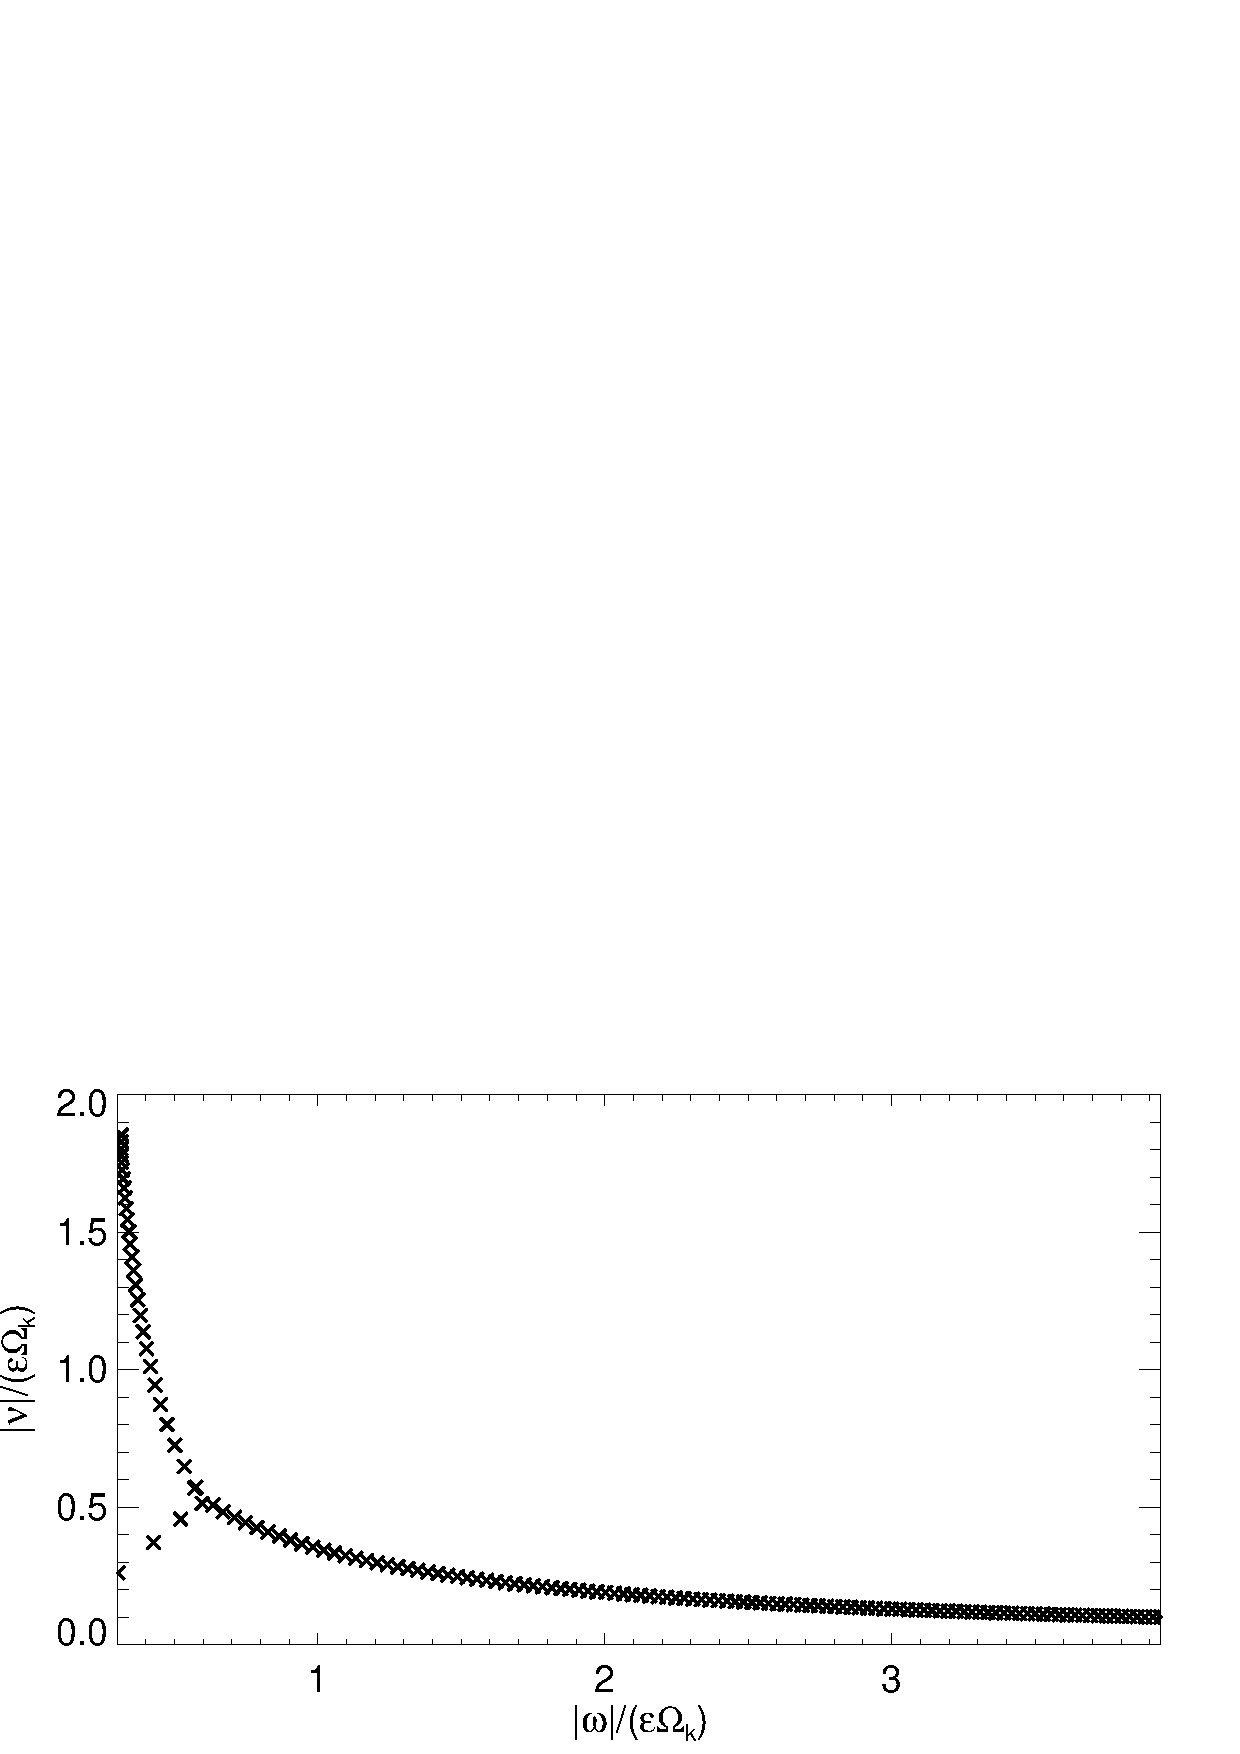
\includegraphics[width=\linewidth]{figures/eigenvalues_iso}
  \caption{Eigenvalues in the low-frequency approximation for the
    vertical shear instability in a vertically isothermal disk evolved
    isothermally ($\gamma=\Gamma=1$). The disk parameters are $q=-1$,
    $p=-1.5$ and $\epsilon=0.1$, while the perturbation radial
    wavenumber is $k_x=200\pi/r$. This is the set up considered in
    \cite{mcnally14}. \label{lowfreq_eigen}
  }
\end{figure}

We plot in Fig. \ref{lowfreq_eigenfunc} the structurally simplest
eigenfunction --- the fundamental corrugation mode corresponding to
the eigenvalue with $\mathrm{min}|\sigma|$. The perturbation $W$ is
roughly proportional to $z$, except close the boundaries where it
flattens because $\delta v_z=dW/dz=0$ is imposed there. 

For $k_x = 200\pi/r$ and $\epsilon = 0.1$, the dimensionless
wavenumber $\hat{k} = k_xH_\mathrm{iso}=20\pi$. Then the expected
growth rate according to Eq. \ref{simple_growth} with $M=1$ is
\begin{align*}
  \nu = 0.2606\epsilon\Omega_k,
\end{align*}
as obtained numerically (Fig. \ref{lowfreq_eigen}). This agreement is
surpsingly good, given that Eq. \ref{simple_growth} assumes the
thin-disk approximation and imposes a different boundary condition to
that in the numerical calculations. 

\begin{figure}
  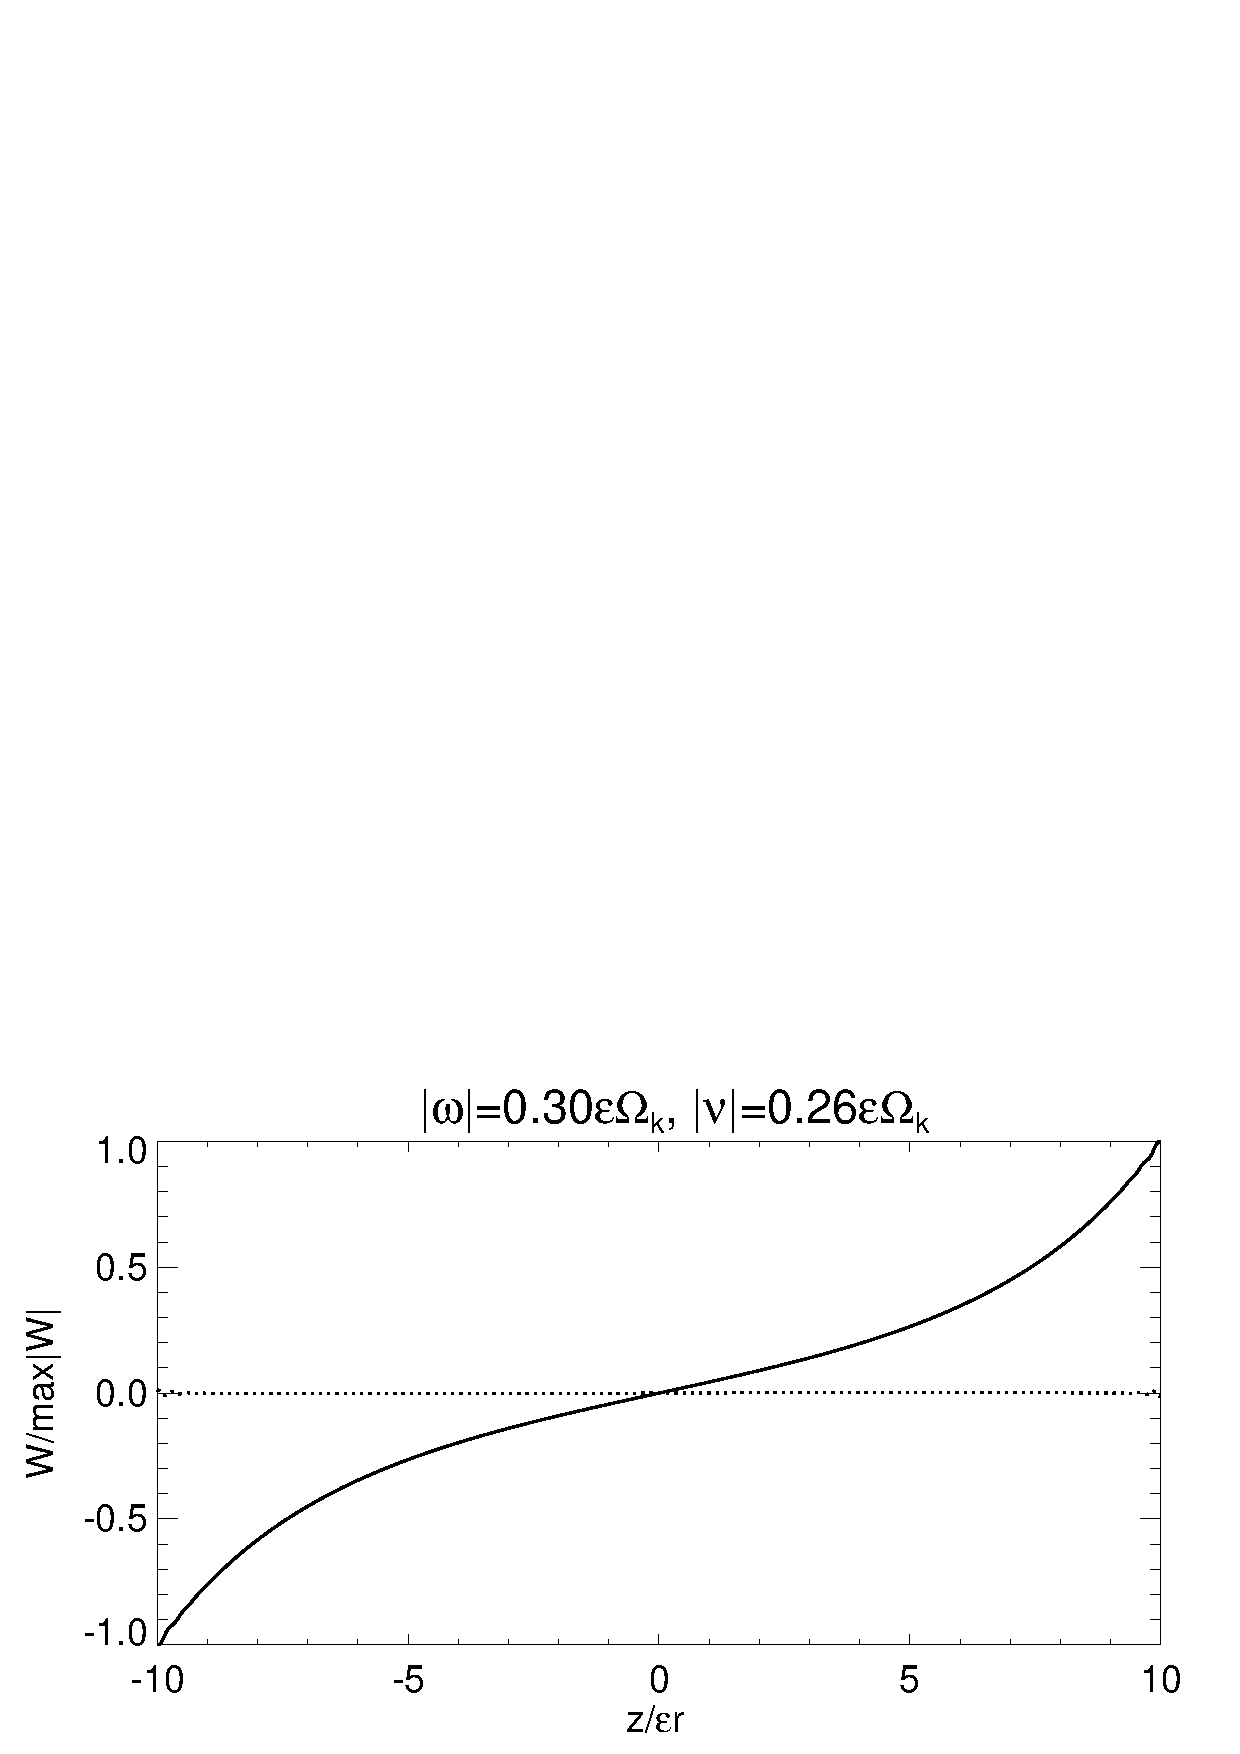
\includegraphics[width=\linewidth]{figures/eigenvector_iso}
  \caption{Eigenfunction of the fundamental corrugation mode,
    corresponding to the 
    bottom-left eigenvalue displayed in Fig. \ref{lowfreq_eigen}. The
    solid and dashed lines are $\real W$ and $\imag W$, respectively. 
    \label{lowfreq_eigenfunc}
  }
\end{figure}

\subsubsection{Influence of vertical boundaries}

\subsection{Adiabatic perturbations} 
We now extend the above discussion to vertically isothermal disks
($\Gamma=1$) with $\gamma\neq1$ and $t_c\to\infty$, i.e. adiabatic
evolution. We eliminate variables in favor of $\delta v_z$ and
$\Delta \equiv \nabla\cdot\delta\bm{v}$ to obtain
\begin{align}
&\Delta\left(1 + \frac{\gamma c_s^2 k_x^2}{D}\right) = \frac{d\delta
  v_z}{dz} + \frac{\ii k_x^2}{D}\left(\ii c_s^2 \frac{d\ln\rho}{dz}
  - \frac{r}{k_x}\frac{d\Omega^2}{dz}\right)\delta v_z,\label{adia_iso1}\\
& -\sigma^2\delta v_z = \gamma c_s^2 \frac{d\Delta}{dz} +
c_s^2\frac{d}{dz}\left(\frac{d\ln\rho}{dz}\delta v_z\right) +
\left(\gamma-1\right)\frac{d\ln\rho}{dz} \Delta.\label{adia_iso2}
\end{align}
{\bf note: incompressible mode, set delta to zero. only works for
  constant gravity.}

We again make the low-frequency approximation
and ignore the vertical dependence of $\Omega$ and $\kappa$ except
where their vertical derivatives appear explicitly in the above
equations. We thus make the replacement $D\to \Omega_k^2$, as before
for isothermal perturbations. Here, we also use
the fact that in the global disk,
\begin{align}
  r\frac{\p \Omega^2}{\p z} = - \frac{\p\ln\rho}{\p z}\frac{\p
    c_s^2}{\p r} = -\frac{\p \ln\rho}{\p z} \frac{qc_s^2}{r},
\end{align}
where the second equality follows from the power-law prescription of
the sound-speed for $\Gamma=1$. 

Combining Eq. \ref{adia_iso1} and Eq. \ref{adia_iso2} with the above
substitutions we obtain, in terms of dimensionless variables defined previously, an equation for $\delta v_z$,
\begin{align}
  0 =& \dd v_z^{\prime\prime} + \left(1 + \ii \epsilon q
    \hat{k}\right)\left(\ln\rho^{\prime}\delta v_z\right)^\prime\notag\\
  &+\left\{\hat{\sigma}^2\left(\frac{1}{\gamma}+\hat{k}^2\right)\right.\notag\\
  &\phantom{0=}\left.-\left(\frac{\gamma-1}{\gamma}\right)\left[\ln\rho^{\prime\prime}+\hat{k}^2\left(1-\frac{\ii\epsilon
          q}{\hat{k}}\right)\ln\rho^{\prime 2}\right]\right\}\delta v_z.\label{adia_iso3}
\end{align}
We multiply Eq. \ref{adia_iso3} by $\rho\delta v_z^*$ and
integrate vertically, assume boundary terms vanish when integrating by
parts, to obtain
\begin{align}
  &\hat{\sigma}^2\left(\frac{1}{\gamma} +
    \hat{k}^2\right)\int_{\zhat_1}^{\zhat_2}\rho|\delta
  v_z|^2 d\zhat \notag\\
  &=  \left(\frac{\gamma-1}{\gamma}\right)
  \int_{\zhat_1}^{\zhat_2}\rho|\delta v_z^\prime|^2 d\zhat
  +\frac{1}{\gamma}\int_{\zhat_1}^{\zhat_2}\frac{1}{\rho}|(\rho\delta
  v_z)^\prime|^2 d\zhat\notag\\
  &\phantom{=} +
  \left(\frac{\gamma-1}{\gamma}\right)\hat{k}^2\left(1-\frac{\ii\epsilon
      q}{\hat{k}}\right) \int_{\zhat_1}^{\zhat_2}\rho\ln\rho^{\prime
    2}|\delta v_z|^2 d\zhat\notag\\
  &\phantom{=} + \ii\epsilon q \hat{k}
  \int_{\zhat_1}^{\zhat_2}\ln\rho^\prime(\rho\delta v_z^*)^\prime
  \delta v_z d\zhat.\label{adia_integral}
\end{align}
When $q\equiv0$, all the terms on the right-hand-side (RHS) are real. Then
$\hat{\sigma}^2$ is real, and  $\hat{\sigma}^2>0$ if $\gamma>1$. As
expected, a sub-adiabatically stratified disk is stable in the absense
of vertical shear. In the presence of vertical shear $q\neq0$ and
$\hat{\sigma}$ is generally complex, which implies the possibility of
instability.  

Note that the term with $\ln\rho^{\prime 2}$ in the integrand (third
term on the RHS) represents stabilization by the vertical entropy
gradient when there is no vertical shear. It gives an imaginary
contribution to $\hat{\sigma}$ when $q\neq0$, but this is a factor
$|\epsilon/\hat{k}|$ smaller than the real (stabilizing) contribution,
since $\epsilon\ll 1$ for a thin disk and we (usually) consider
$\hat{k}\gg1$. Thus, instability is expected to be due to the 
last term on the RHS of Eq. \ref{adia_integral}. 
  
\subsubsection{Explicit solutions in the thin-disk limit}
To simplify further, we consider the problem in the thin-disk limit so
that $\ln \rho \simeq -\zhat^2/2$. Eq. \ref{adia_iso3} becomes 
\begin{align}
  0 = \delta v_z^{\prime\prime} - \zhat A \delta v_z^\prime + \left(B
    - C \zhat^2\right)\delta v_z,
\end{align}
with
\begin{align}
  &A \equiv 1 + \ii \epsilon q \hat{k},\\
  &B \equiv \hat{\sigma}^2\left(\frac{1}{\gamma} + \hat{k}^2\right) -
  \left(\frac{1}{\gamma} + \ii \hat{k} \epsilon q\right)\\
  &C \equiv \frac{\left(\gamma-1\right)}{\gamma}\hat{k}^2\left(1 - \frac{\ii
      \epsilon q}{\hat{k}}\right).\label{adia_thin}
\end{align}
Let
\begin{align}
  \delta v_z(\zhat) =
  g(\zhat)\exp\left(\frac{\alpha\zhat^2}{2}\right), \label{adia_ansatz}
\end{align}
where $\alpha$ is a constant to be chosen for convenience. We require
the vertical kinetic energy density $\rho|\delta v_z|^2$ to remain
finite.  Then assuming
$g(\zhat)$ is a polynomial, we require 
\begin{align}
  \real\alpha < \frac{1}{2}. 
\end{align}

Inserting the ansatz Eq. \ref{adia_ansatz} into Eq. \ref{adia_thin}
gives
\begin{align}
  0 = g^{\prime\prime} - \hat{z}\left(A - 2\alpha\right)g^\prime + \left(B +
      \alpha\right)g
    +\underbrace{\left(\alpha^2 - \alpha A - C\right)}_\text{set to zero}\zhat^2 g.
\end{align}
We choose $\alpha$ to make the coefficient of $\zhat^2g$ vanish. That
is,
\begin{align}
  \alpha = \frac{1}{2}\left(A - \sqrt{A^2 + 4C}\right).
\end{align} 
We now have an equation in the same form as Eq. \ref{iso_ode3}:
\begin{align}
  0 = g^{\prime\prime} - \hat{z}\left(A - 2\alpha\right)g^\prime +
  \left(B + \alpha\right)g.
\end{align}
We seek polynomial solutions 
\begin{align}
  g(\zhat) = \sum_{m=0}^M b_m \zhat^m,
\end{align}
% We again seek power-series solutions 
% \begin{align}
%   g(\zhat) = \sum_{m=0}^\infty b_m \zhat^m,
% \end{align}
% which requires
% \begin{align}
%   (m+2)(m+1)b_{m+2} + \left[\left(2\alpha - A\right)m + B + \alpha\right]=0.
% \end{align}
which requires
\begin{align}
  B + \alpha = M\left(A-2\alpha\right).
\end{align}
Inserting the definition of $B$ we get
\begin{align}
  &\hat{\sigma}^2\left(\frac{1}{\gamma}+\hat{k}^2\right) \notag\\ &=
  \left(\frac{1}{\gamma}-\frac{1}{2}\right) +\frac{\ii}{2}\epsilon q
  \hat{k} + \frac{1}{2}\left(2M+1\right)\left(A^2 + 4C\right)^{1/2}\label{adia_disp}. 
\end{align}
%Recalling that $B$ depends $\hat{\sigma}$, Eq. \ref{adia_disp} gives
%the eigenfrequency as a function of disk paramters. 


\subsubsection{The case of $\gamma=2$}
In principle, we can solve Eq. \ref{adia_disp} for the mode
frequencies and growth rates. This is complicated in 
general, but simplifies for $\gamma=2$, for which the quantity
$A^2+4C$ is real. In this case we find
\begin{align}
  \hat{\nu}^2 =
  \frac{1}{2}\frac{(2M+1)}{\sqrt{1+2\hat{k}^2}}&\left[
    \sqrt{1-\frac{4M(M+1)\hat{k}^2\epsilon^2q^2}{(2M+1)^2(1+2\hat{k}^2)}}\right.\notag\\
  &\phantom{=}
  \left.- \sqrt{1 - \frac{\hat{k}^2\epsilon^2q^2}{(1+2\hat{k}^2)}}\right].
\end{align}
In the limit of a thin disk $\epsilon\to0$ or weak shear $|q|\to0$, we
have
\begin{align}
  \hat{\nu}^2 = \frac{\epsilon^2
    q^2}{4(2M+1)}\frac{\hat{k}^2}{(1+2\hat{k}^2)^{3/2}},\label{gam2_growth}
\end{align}
and the maximum growth rate occurs at $\hat{k}=\hat{k}_\mathrm{opt}=1$,  
\begin{align}
  \mathrm{max}(\hat{\nu}) &= \frac{|\epsilon
    q|}{2(3^{3/4}\sqrt{2M+1})}\label{gam2_max_growth}.
  % & \leq \frac{|\epsilon
  % q|}{2\times3^{3/4}}\notag.
\end{align}
Eq. \ref{gam2_max_growth} show that growth rates decrease with $M$,
and there exists a maximum possible growth rate at $M=0$. This is
despite the fact that in the thin-disk approximation, for which
$d\Omega^2/dz\propto z$, there is infinite vertical shear
available.  

\subsubsection{Comparison with $\gamma=1$}
We can compare growth rates obtained for $\gamma=2$ to those for
$\gamma=1$ in the previous section. If we compare growth rates at their 
respective optimum radial wavelengths, we find
that for $\gamma=2$ the \emph{maximum} possible growth rate, occuring
at $M=0$, is still $\sim2$ times smaller than the \emph{minimum} growth
rate for $\gamma=1$. That is,
\begin{align}
  &\mathrm{max}(\hat{\nu}) \geq \frac{|\epsilon q|}{2\sqrt{1+|\epsilon
      q|}} & \text{at }\hat{k} = \hat{k}_\mathrm{opt} \text{ for }   \gamma=1,  \\
  &\mathrm{max}(\hat{\nu}) \leq \frac{|\epsilon q|}{2\times 3^{3/4}}
           & \text{at }\hat{k} = \hat{k}_\mathrm{opt} \text{ for } \gamma=2.
\end{align}

We can also compare growth rates in the limit $\hat{k}\gg1$ using
Eq. \ref{simple_growth} and Eq. \ref{gam2_growth},
\begin{align}
  &\hat{\nu} \geq \sqrt{\frac{|\epsilon q|}{2\hat{k}}}
  &  \text{as }  \hat{k}\to\infty  \text{ for }  \gamma=1, \\
  &\hat{\nu} \leq \frac{|\epsilon q|}{2^{7/4}\sqrt{\hat{k}}}
  &\text{as }  \hat{k}\to\infty  \text{ for }  \gamma=2.
\end{align}
Then the growth rate of perturbations with large $|\hat{k}|$ in a
$\gamma=2$ disk is at most $2^{-5/4}\sqrt{|\epsilon q|}$ times that in a
$\gamma=1$ disk. For $\epsilon = 0.1$ and $|q|=1$, this factor is
$\sim 0.1$.  

In Fig. \ref{adia_growth} we plot the growth rate $|\hat{\nu}|$ as a
function of the radial wavenumber $\hat{k}$, for a range of adiabatic
indices, using Eq. \ref{adia_disp}. The presence of a positive
vertical entropy gradient is strongly stabilizing. This is because the
vertical shear grows as $z$ away from the midplane (and has a maximum
when the thin-disk approximation is relaxed), but the
square of the bouyancy frequency, which is stabilizing, grows as $z^2$
away from the midplane. The entropy $P/\rho^\gamma$ formally diverges
for $z\to\infty$ even without the thin-disk approximation.        

\begin{figure}
  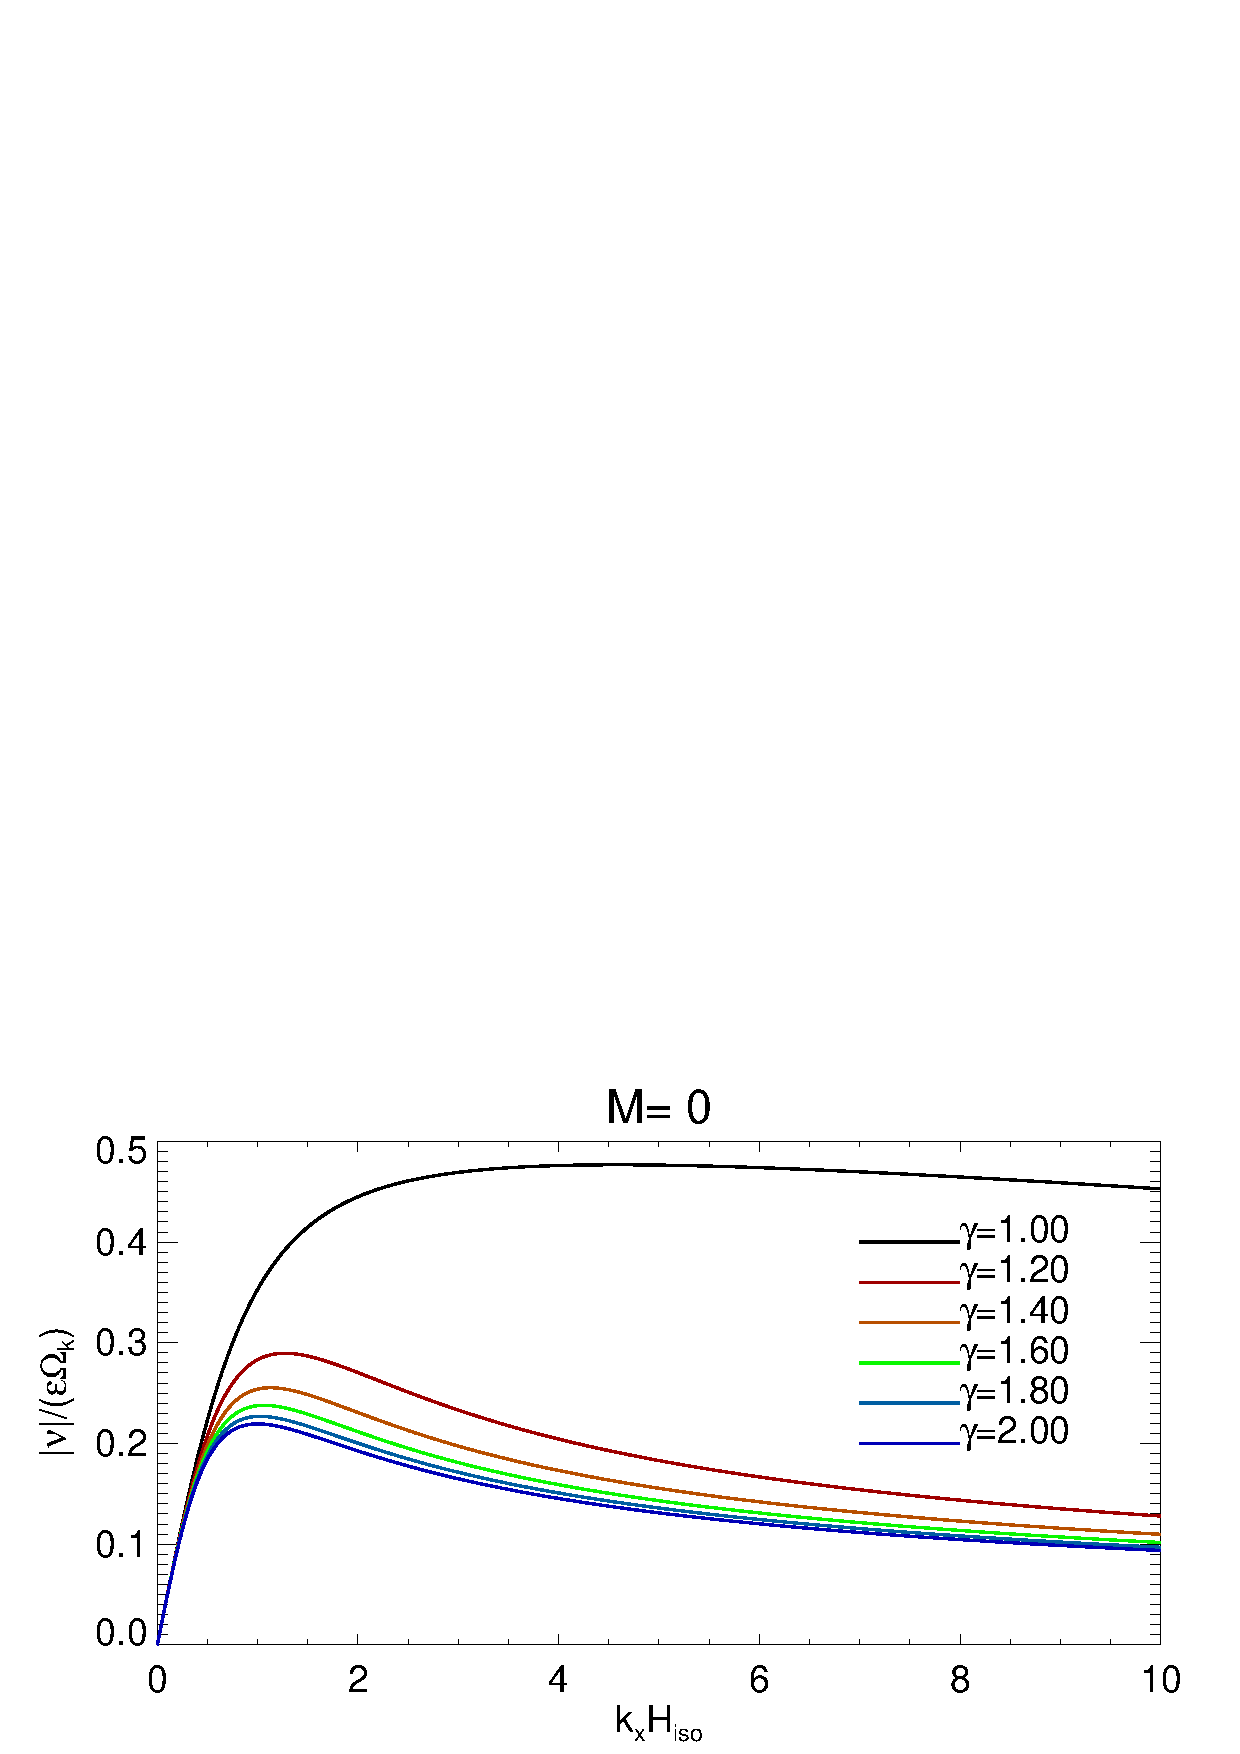
\includegraphics[width=\linewidth]{figures/rate_theory_gmma}
  \caption{Growth rate of the fundamental VSI mode in vertically
    isothermal disks ($\Gamma=1$) subject to adiabatic perturbations,
    calculated in thin disk approximation from Eq. \ref{adia_disp}
    with $M=0$, $\epsilon=0.1$ and  
    $|q|=1$. Growth rates are shown as a function of the radial
    wavenumber for different values of the adiabatic index
    $\gamma$. For $\gamma\equiv 1$ the perturbations are isothermal
    and there is no vertical entropy gradient.\label{adia_growth}}  
\end{figure}   
\section{Numerical solutions}
In this section we numerically solve the linear stability problem
corresponding to Eq. \ref{lin_mass}---\ref{lin_energy}. 
We relax the thin-disk, low-frequency and nearly-Keplerian
approximations used in the analytical discussion above, and  
use the full expressions of $\rho$, $\Omega$ and
$\kappa$ given in \S\ref{eqm}. We also restore $\hat{g}_c=1$ to
account for the background radial disk structure.  

%, so that we may consistently consider vertical domains up to
%$z\sim r$.   

We solve the linear problem by expanding the
perturbations in Chebyshev polynomials $T_l$ up to $l=512$
and discretizing the equations on a grid with
$z\in[-\zmax,\zmax]$. At the vertical boundaries we impose a free
surface, 
\begin{align}
  \Delta P \equiv \delta P + \bm{\xi}\cdot\nabla P= 0 \quad \text{at } z=\pm\zmax,
\end{align}
where $\bm{\xi}$ is the Lagrangian displacement. This boundary
condition is convenient for numerical implementation since it conforms
to a standard eigenvalue problem. The above discretization procedure
converts the linear system of differential equations to a set of 
algebraic equations, for which we use matrix routines in the LAPACK
package to solve. 

% mention mode selection -> focus on fundamental corrugation ->
% simulations eventually dominated by them 
% choice of kx is O(10), since nelson observe kxH \sim 30
%not possible to survey all modes/kx/disk parameters
%focus on effect of thermal relaxation

\subsection{VSI in a locally isothermal, neutrally stratified disk}\label{vertiso_pertiso} 
% disk model is a nearly-vertically
% isothermal disk with $\Gamma=1.011$, $p=-1.5$, $q=-1$,
% $\epsilon=0.1$. 
We first calculate the VSI in a nearly vertcally isothermal, neutrally
straitified disk ($N_z^2\equiv0$) by setting
$\gamma=\Gamma=1.011$ and $\beta=10^{-3}$. Other disk parameters are 
$(p,q,\epsilon)=(-1.5,-1,0.1)$ and the vertical domain is $\zmax =
5\epsilon r$. This setup is similar to that adopted in
\cite{mcnally14}, who calculated the VSI in vertically isothermal
disks subject to isothermal perturbations ($\Gamma=\gamma=1$).  This
allows us to test our numerical code.  

%behaviour as func of kx 

Fig. \ref{iso_eigen_kx} compares the numerically-obtained eigenvalues
for the fundamental mode and that calculated from 
Eq. \ref{sig2_iso} (with $L=1$). There is good agreement for 
$\khat\gtrsim10$. The match worsens for smaller $\khat$ because the 
the low-frequency approximation used to obtain Eq. \ref{sig2_iso} 
is no longer valid, as $|\omega|$ is not small compared to $\Omega_k$
for $\khat\lesssim 10$.  

% This means
% that our analytic results should only be applied to perturbations with
% $\khat\gg 1$, i.e. small radial-lengthscales. 

\begin{figure}
  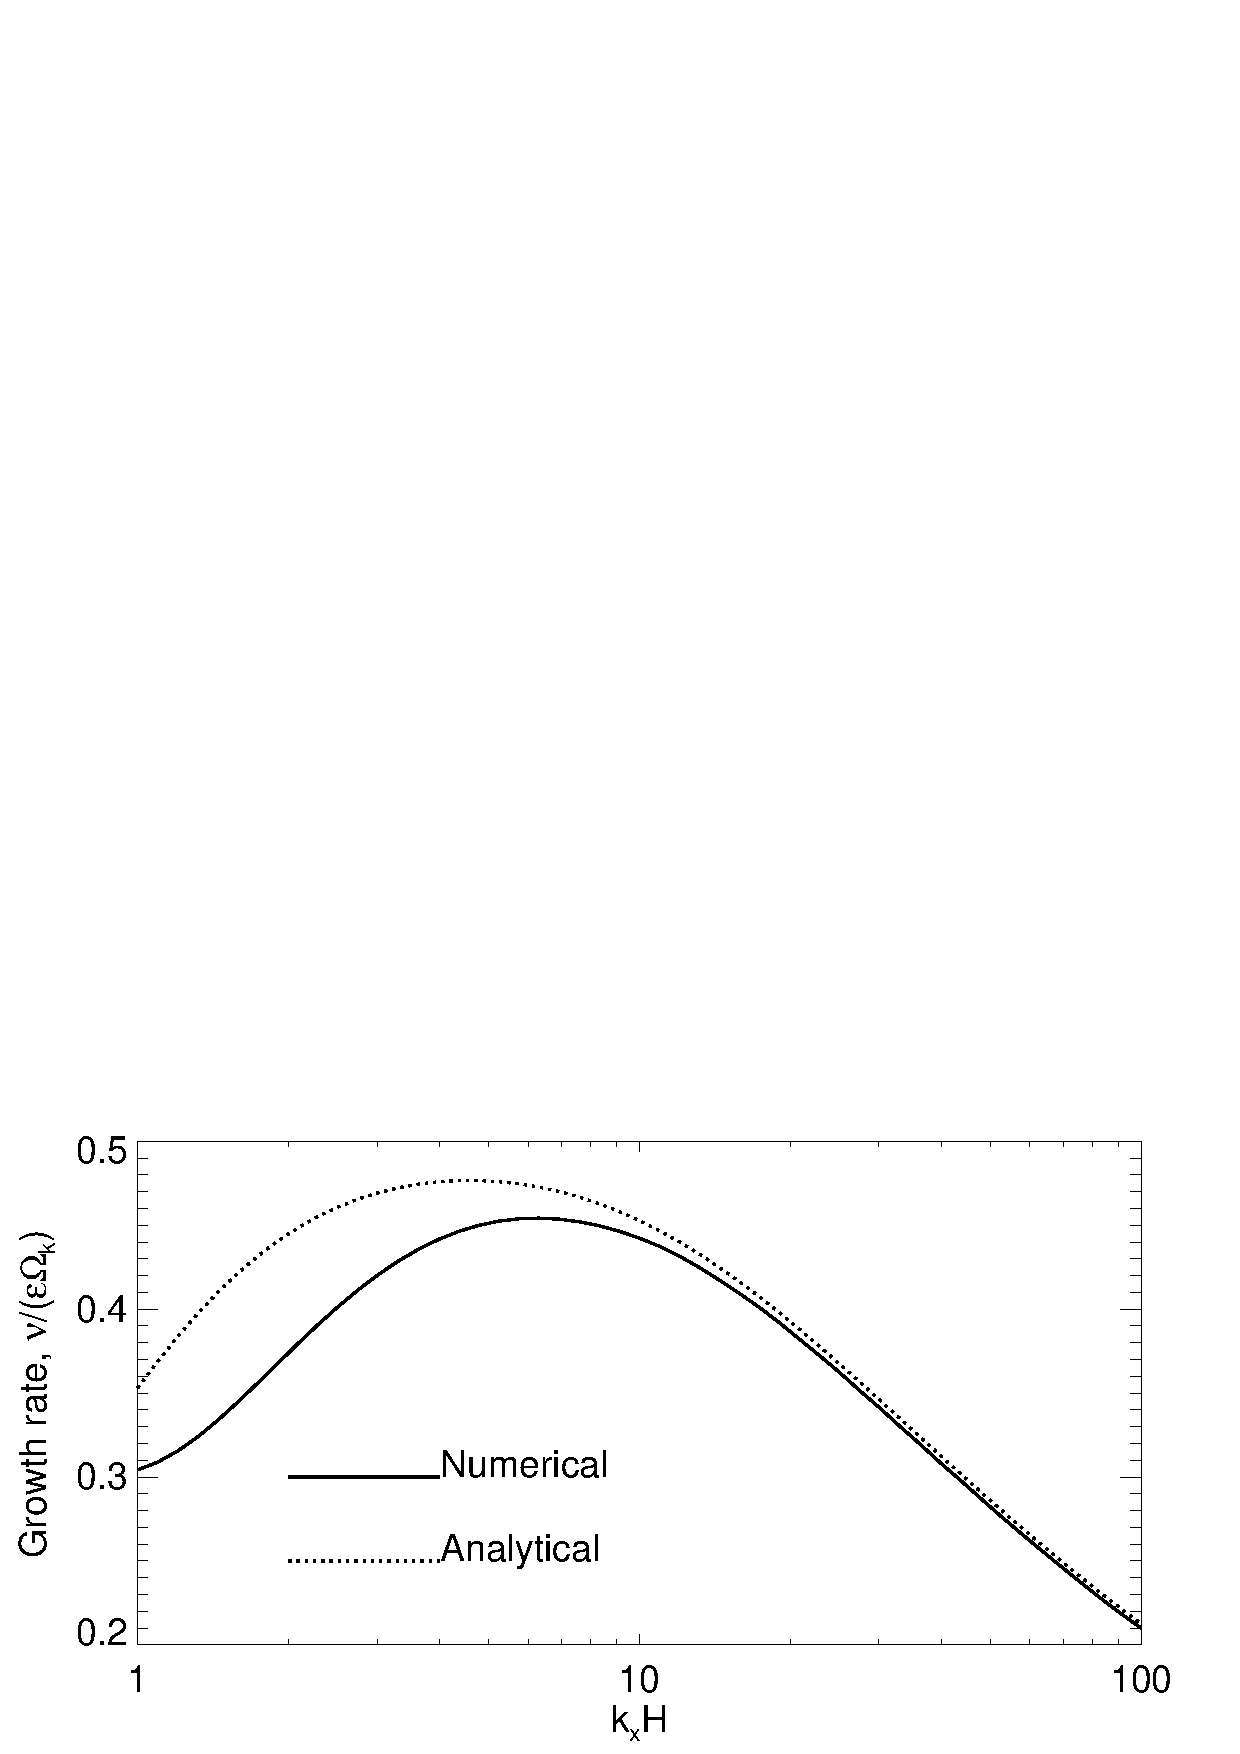
\includegraphics[width=\linewidth,clip=true,trim=0cm 1.75cm 0cm
  0cm]{figures/compare_eigen_imag_iso} 
  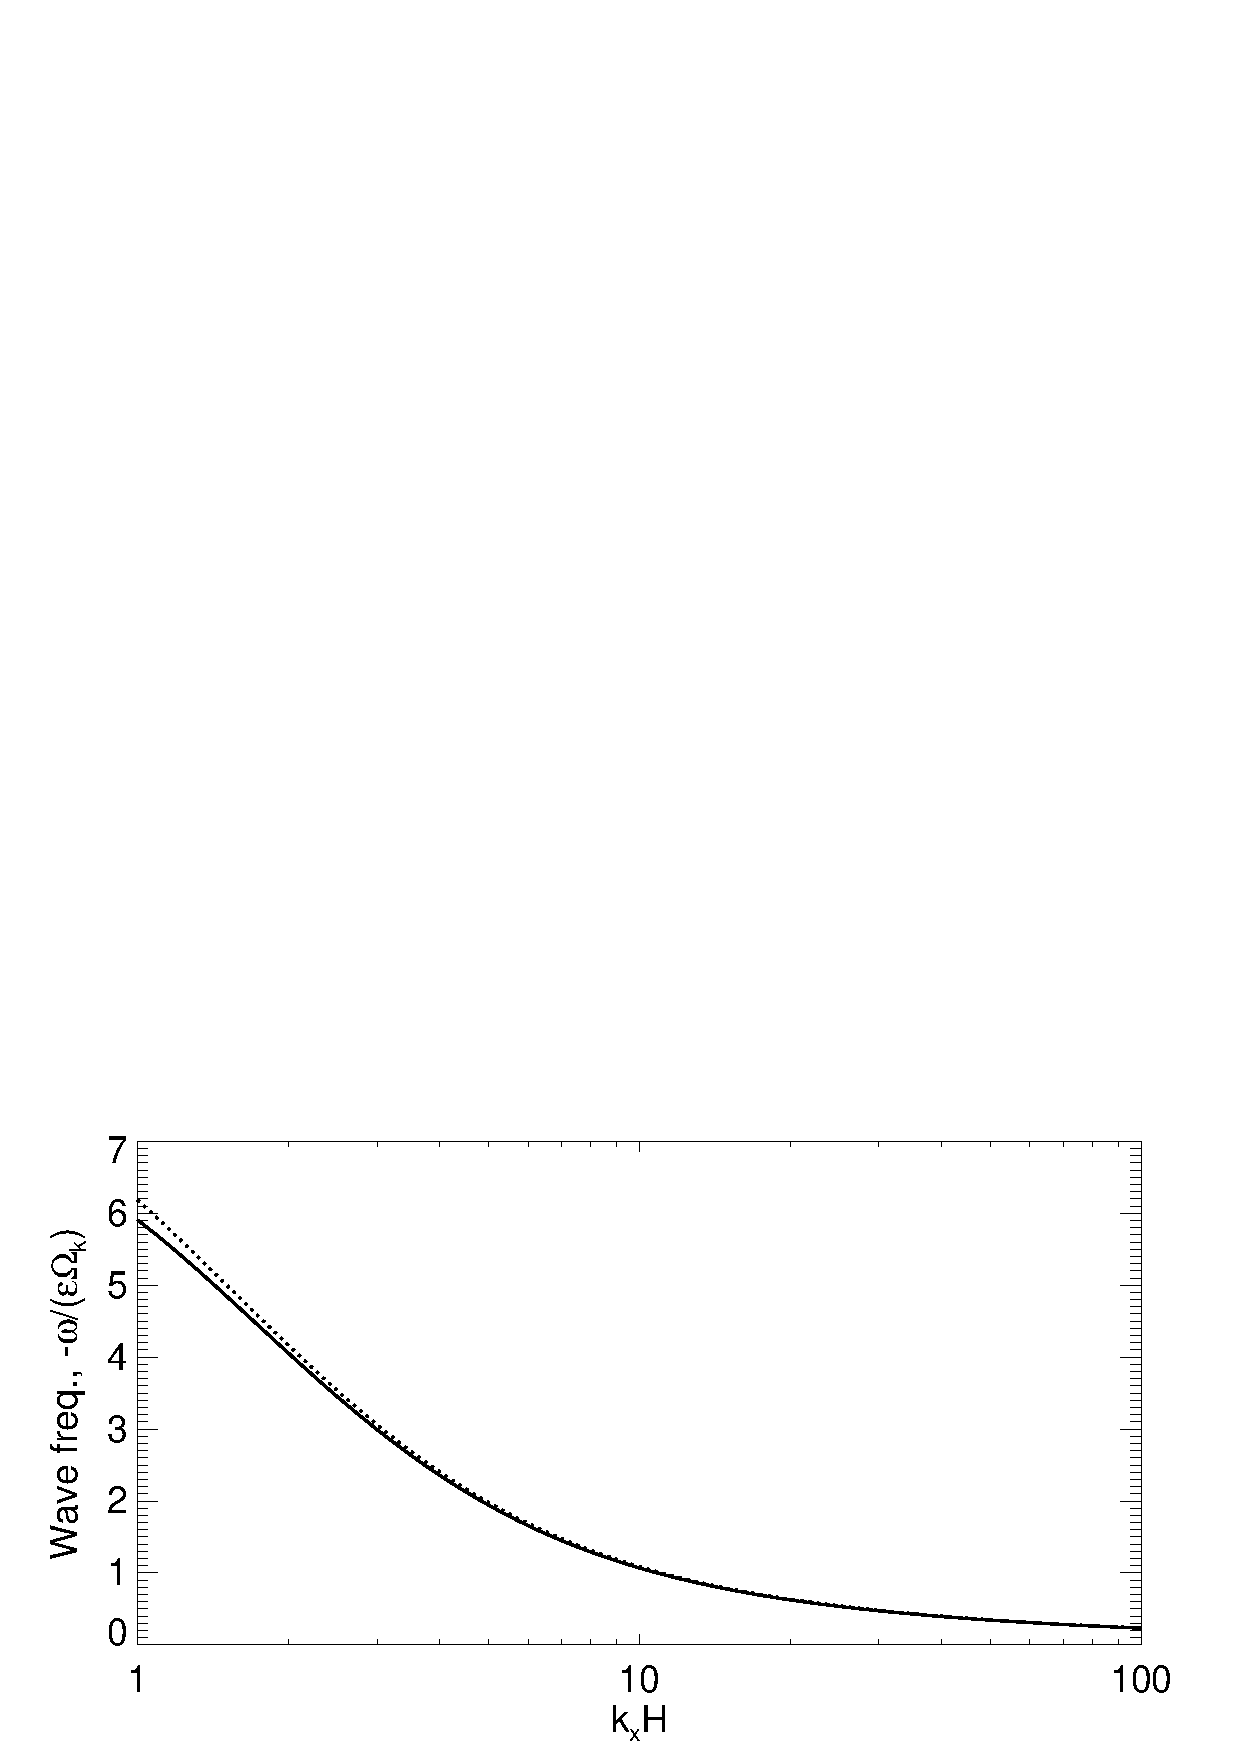
\includegraphics[width=\linewidth,clip=true,trim=0cm 0cm 0cm
  1cm]{figures/compare_eigen_real_iso}
  \caption{Growth rate (top) and real frequency (bottom) of the
    fundamental VSI mode in a disk with $\gamma=\Gamma=1.011$,
    $(p,q,\epsilon)=(-1.5,-1,0.1)$ and
    $\beta=10^{-3}$. The solid (dotted) line is obtained numerically
    (analytically).  
    \label{iso_eigen_kx} 
  }
\end{figure}

Fig. \ref{lowfreq_eigenfunc} compares the fundamental VSI eigenfunction
$W$ for $\khat=1$ and $\khat=20\pi$. The latter value, corresponding
to $k_x= 200\pi/r$, was used by \cite{mcnally14}. We find $W$ is
similar for all $\khat\gtrsim10$ and is proportional to $z$, as
expected for the fundamental mode according to explicit solutions
developed in \S\ref{iso_poly}.  

However, for $\khat\lesssim 10$, e.g. $\khat=1$ in 
Fig. \ref{lowfreq_eigenfunc}, the perturbation magnitude near the
boundaries begin to dominate. For even smaller $\khat\lesssim 1$ (not
shown) we find the perturbation is almost entirely concentrated at the
boundaries. Our radially-local approximation is not valid for 
these small wavenumber perturbations and we do not consider such modes
further.      

\begin{figure}
  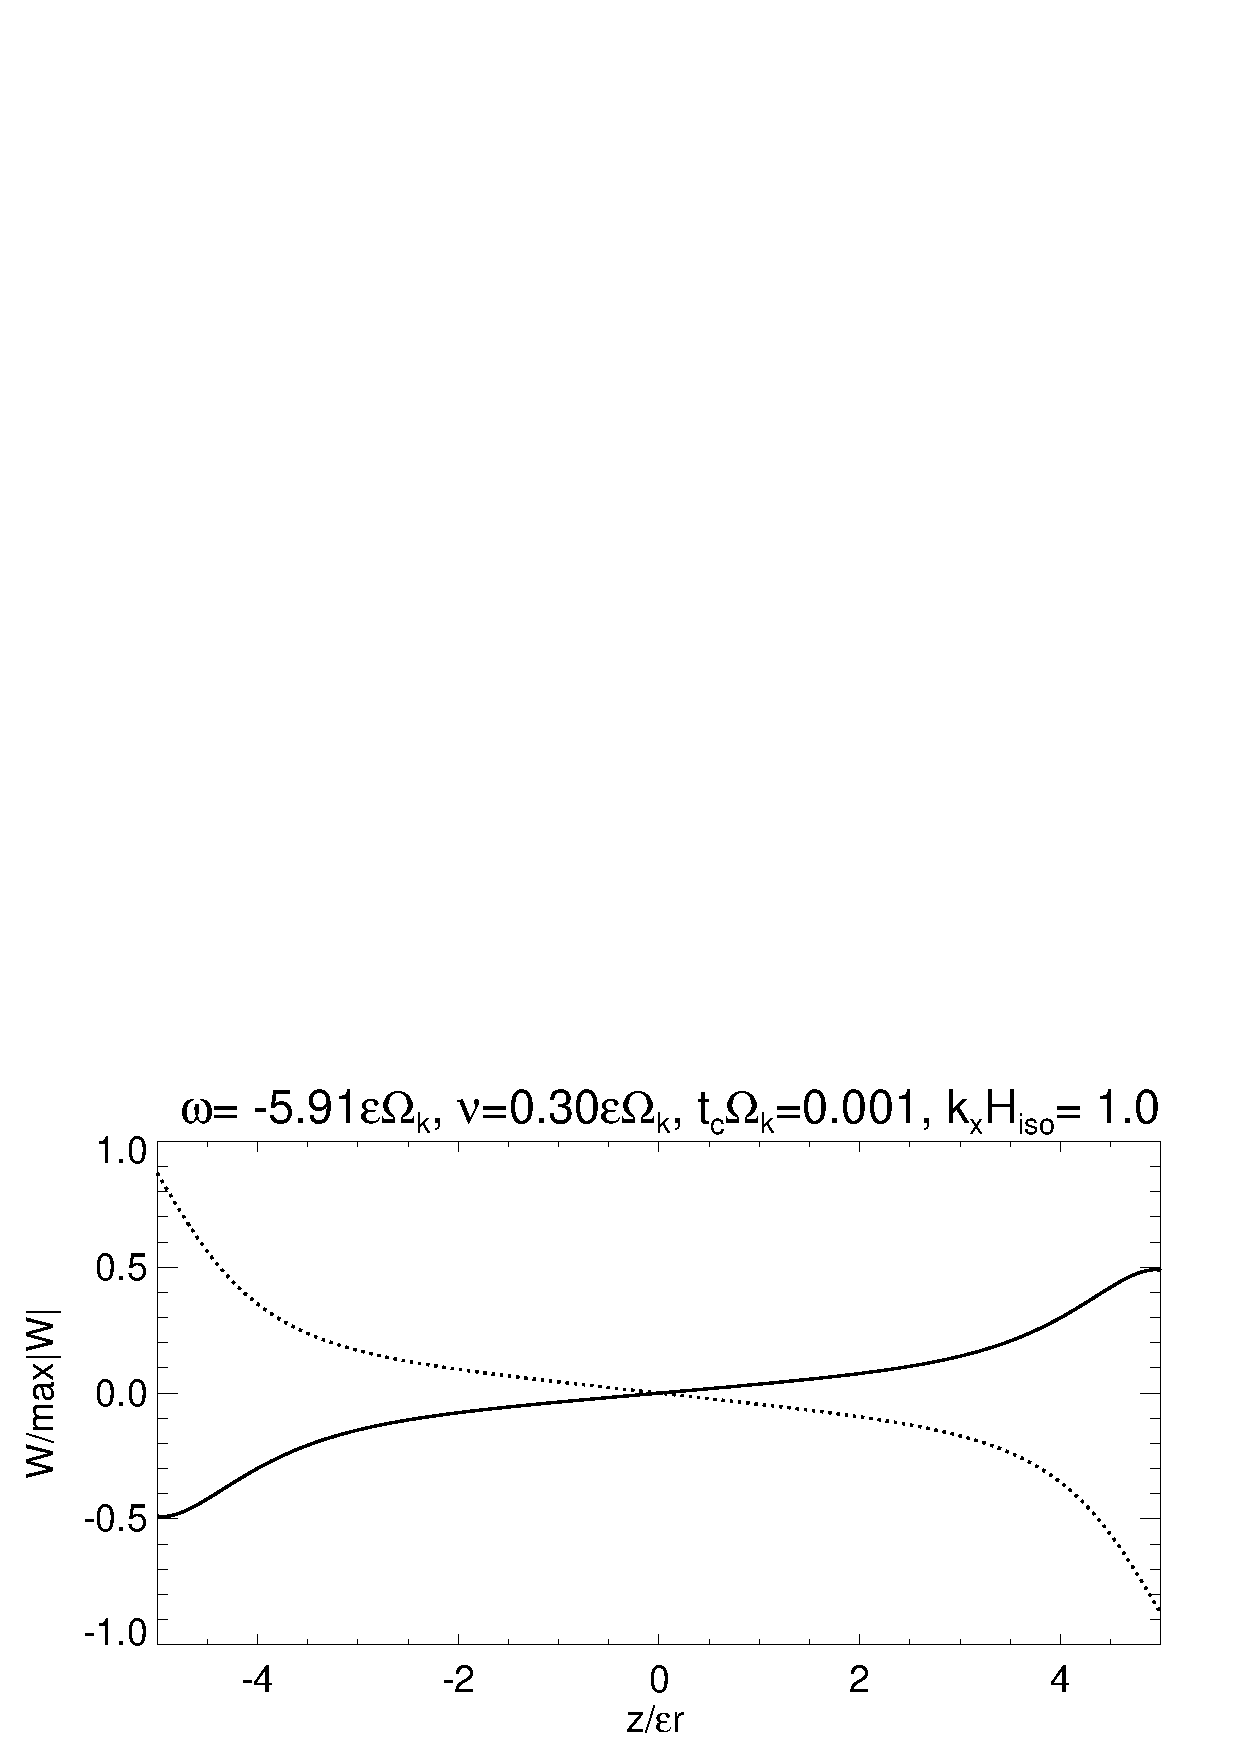
\includegraphics[width=\linewidth,clip=true,trim=0cm 1.75cm 0cm
  0cm]{figures/eigenvector_iso_kx1} 
  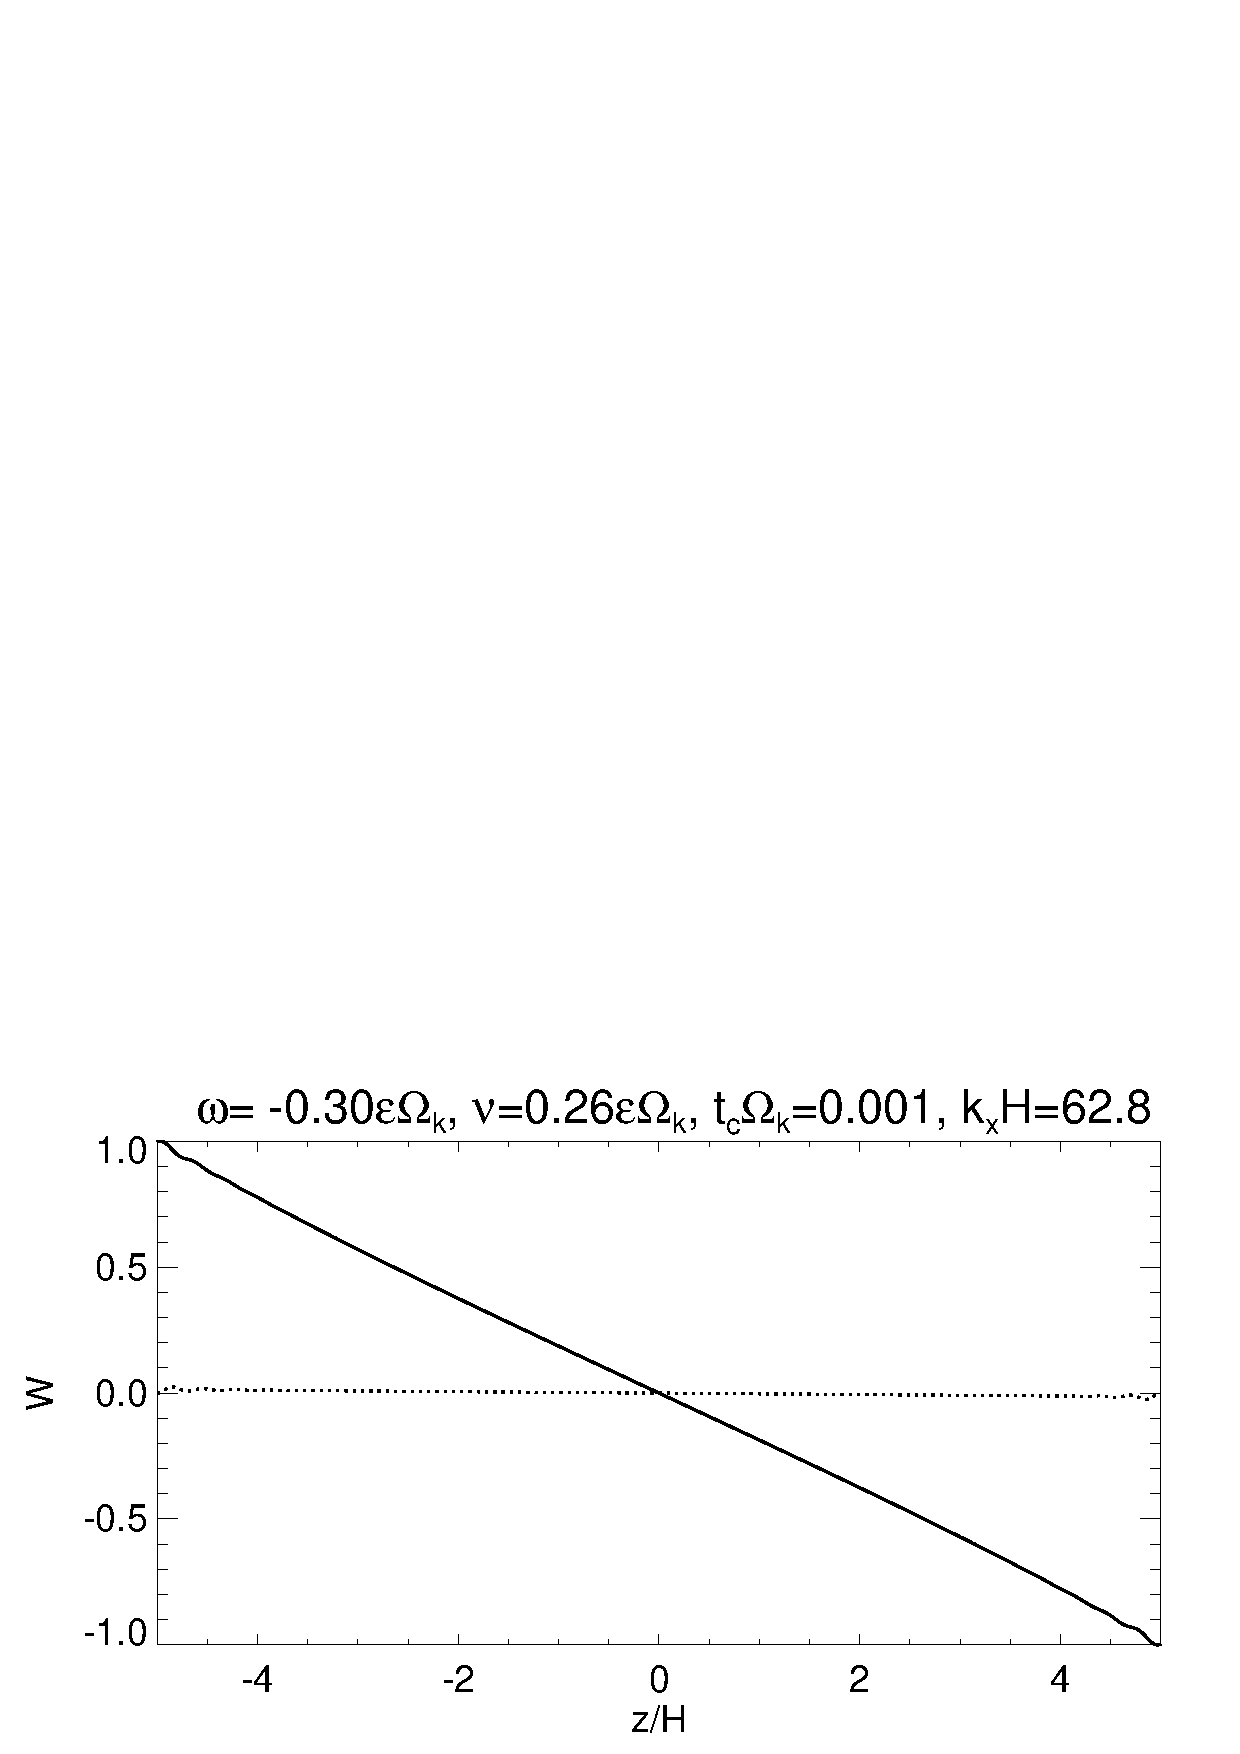
\includegraphics[width=\linewidth]{figures/eigenvector_iso_kx60}
  \caption{Eigenfunction of the fundamental VSI for perturbation
    wavenumber $\khat=1$ (top) and $\khat=20\pi$ (bottom). The real 
    (imaginary) parts of $W$ are plotted as solid (dotted) lines. 
    \label{lowfreq_eigenfunc}
  }
\end{figure}

In Fig. \ref{lowfreq_eigen} we plot the eigenvalues 
$\sigma = \omega + \ii\nu$ found for $\khat=20\pi$. This plot is
similar to Fig. 3 in \cite{mcnally14}. The fundamental
VSI mode, with one node in $W$, has the smallest $|\sigma|$. The
eigenvalue calculated from Eq. \ref{sig2_iso} with $L=1$ and the 
numerically-obtained value are  
\begin{align*}
  (\omega,\nu) = (-0.3053,0.2606)\epsilon\Omega_k &\quad \text{(from
    Eq. \ref{sig2_iso})},\\
  (\omega,\nu) = (-0.3010,0.2575) \epsilon \Omega_k &\quad \text{(numerical)}.
\end{align*}
This agreement is surpsingly good given the number of approximations
used to obtain Eq. \ref{sig2_iso}, which also imposes a different
boundary condition to that in the numerical calculation. These values
are also close to that found by \cite{mcnally14}. The eigenfrequency
is not sensitive to the vertical boundary condition because the
expression for $\sigma$, given by Eq. \ref{integral_relation1},
involve integrands with $\rho$ as the   weight function, which rapidly
decays away from the midplane. 

\begin{figure}
  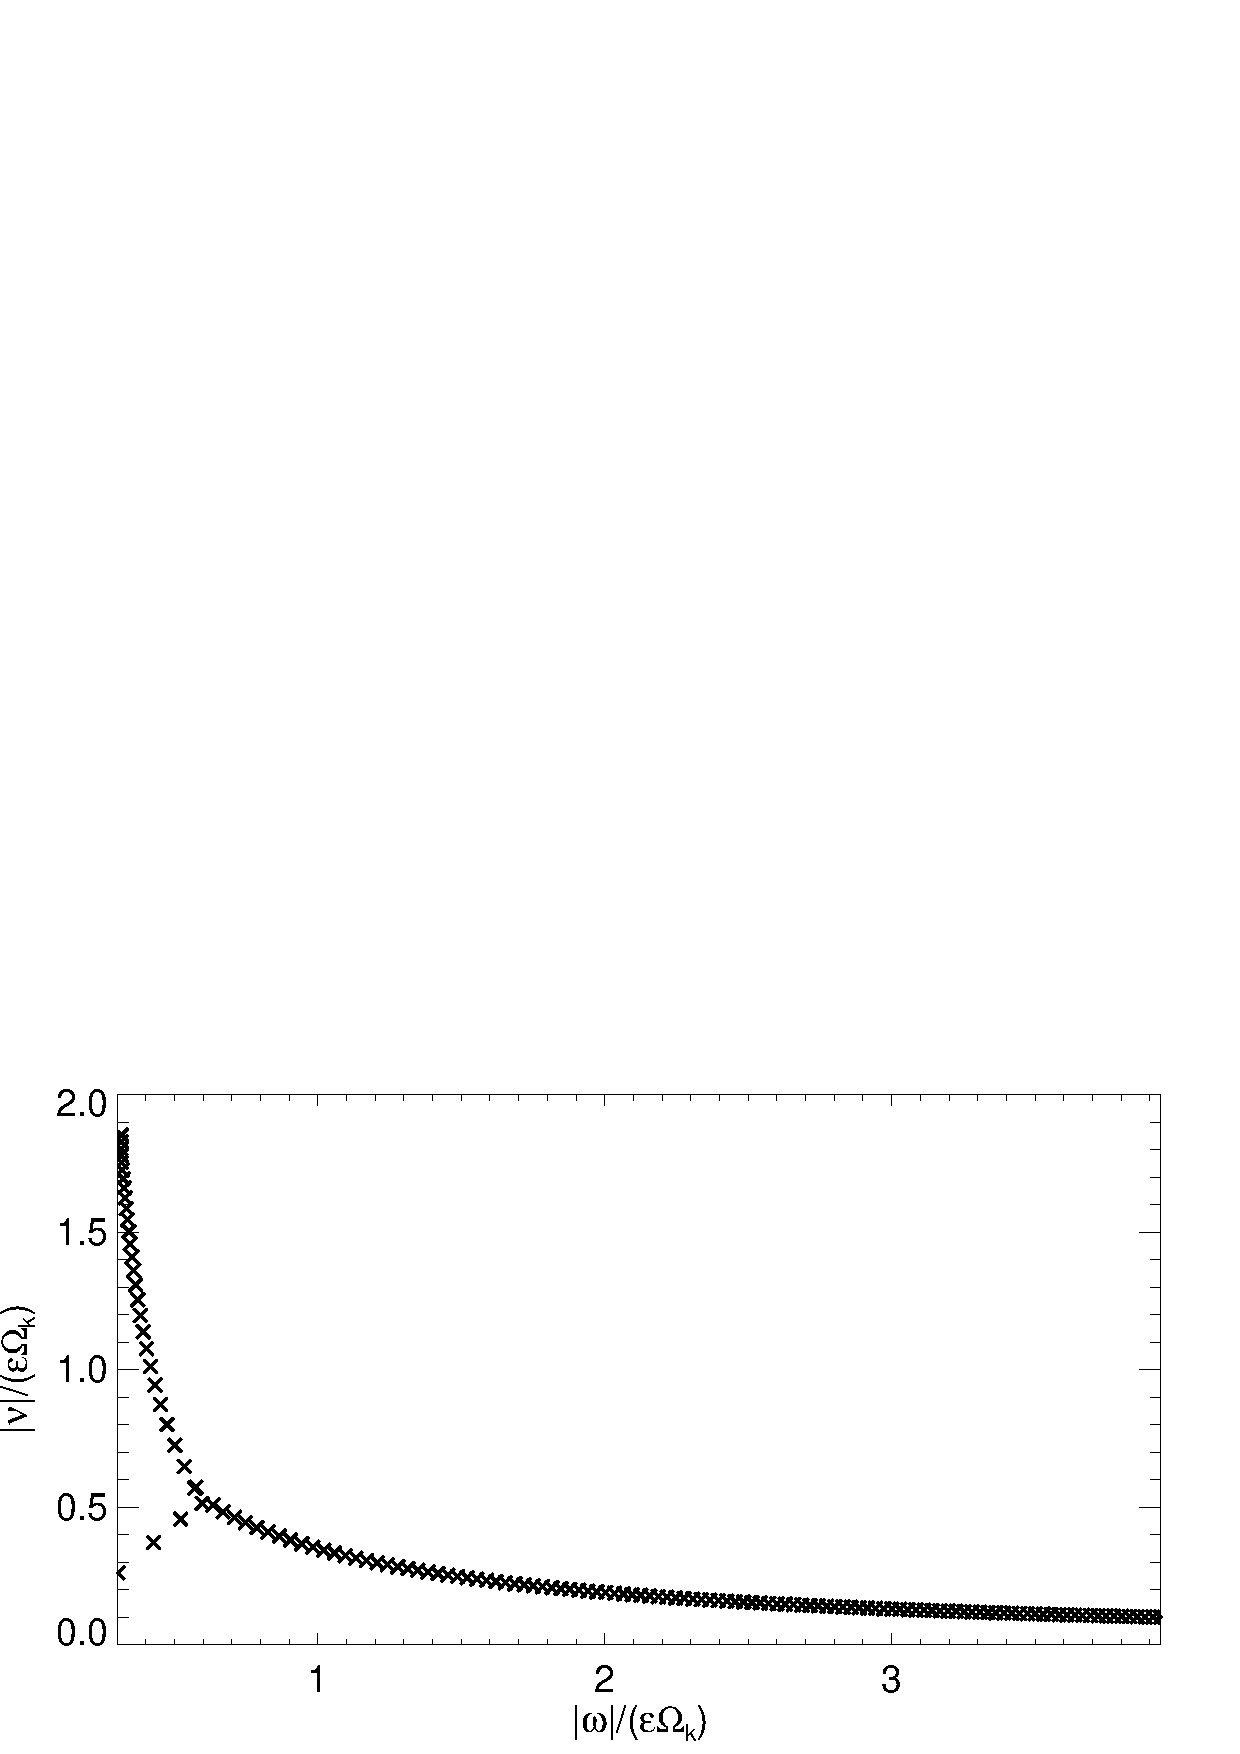
\includegraphics[width=\linewidth]{figures/eigenvalues_iso}
  \caption{Eigenvalues of perturbations with wavenumber $\khat=20\pi$
    in a neutrally-stratified, nearly-vertically isothermal disk
    ($\gamma=\Gamma=1.011$) with $(p,q,\epsilon)=(-1.5,-1,0.1)$ and
    $\beta=10^{-3}$. \label{lowfreq_eigen} 
  }
\end{figure}

\subsection{Effect of thermal relaxation}
We now consider stably stratified disks ($\gamma > \Gamma$) with
thermal relaxation. Here, we use a slightly  
different disk model with $\epsilon=0.05$ and $\gamma=1.4$, as 
adopted in simulations performed by \cite{nelson13}. Other parameters 
are unchanged from the previous section.  

Fig. \ref{bcrit_compare1} shows the growth rate $\nu$ of the
fundamental VSI as a function of $\beta$ for $\khat\in[1,10^2]$. We
also plot the critical thermal relaxation timescale
$\beta_\mathrm{crit}$ given by Eq. \ref{iso_vsi_cond}. For the present
disk parameters $\beta_\mathrm{crit}=0.125$.   

For $5\lesssim\khat\lesssim30$, we find $\beta_\mathrm{crit}$ provides an
accurate prediction of the upper limit to the thermal relaxation 
timescale for  the fundamental mode. For smaller $\khat$,
$\beta<\beta_\mathrm{crit}$ is a sufficient condition for
instability. For larger $\khat$, we find $\nu$ does not reach zero but
rapidly decreases as $\beta$ approaches and increases beyond
$\beta_\mathrm{crit}$. In the latter case we find the perturbation is
concentrated at the vertical boundaries, which may play a role not
accounted by our analytical discussion. 

Fig. \ref{bcrit_compare1} shows that 
$\beta_\mathrm{crit}$ is a good indication for the maximum
thermal relaxation timescale to permit the fundamental VSI. For
$\beta\lesssim O(10^{-2})$, growth rates are insensitive to thermal
relaxation. For this disk model, \citeauthor{nelson13}
found a thermal relaxation timescale of $\beta\gtrsim 0.6$ stabilized
the VSI in non-linear hydrodynamic simulations. This is consistent
with our results.   

%implications for nonlinear sims?

 \begin{figure}
   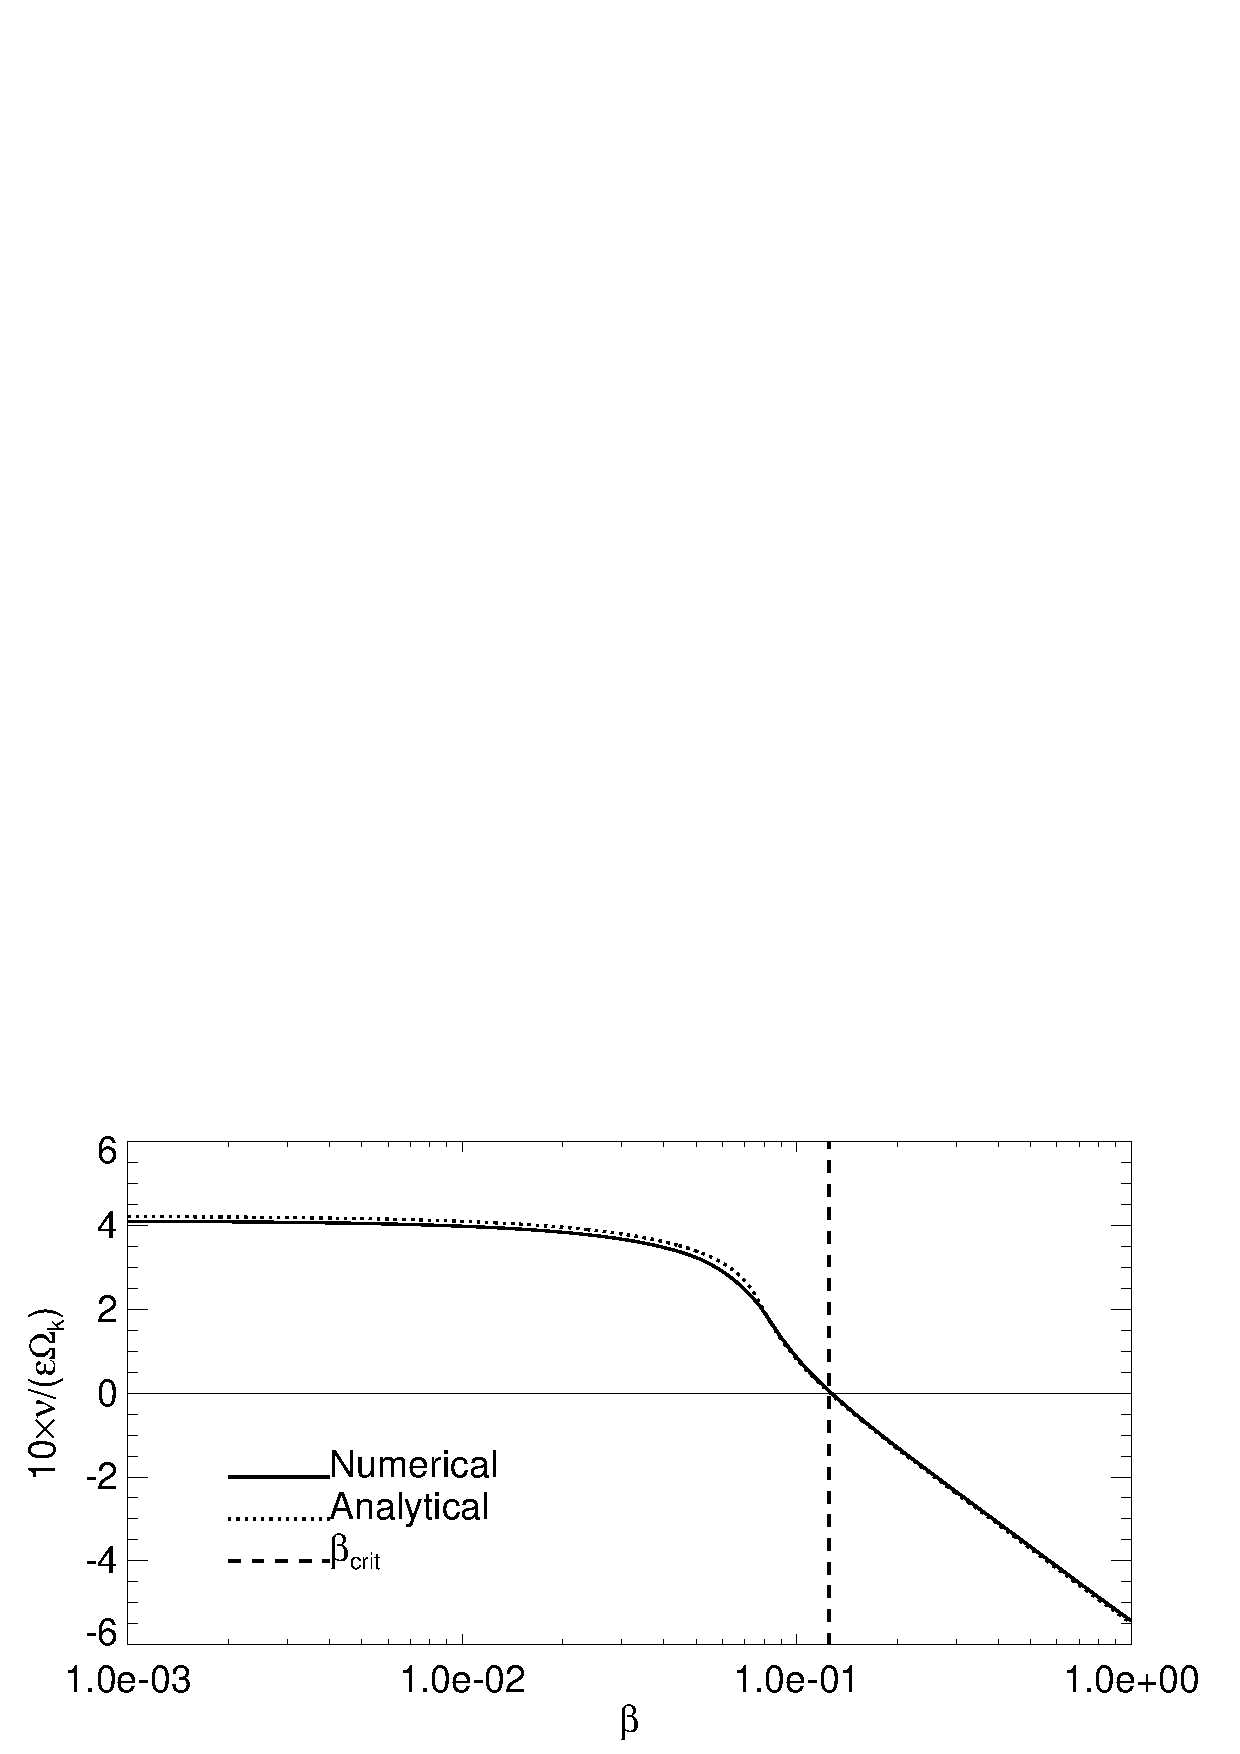
\includegraphics[width=\linewidth]{figures/bcrit_compare} 
   \caption{Growth rate of the fundamental VSI as
     a function of the thermal relaxation timescale $\beta$. The disk
     parameters are $\Gamma=1.011$, $\gamma=1.4$, and 
     $(p,q,\epsilon)=(-1.5,-1,0.05)$. The vertical line
     is the critical thermal timescale $\beta_\mathrm{crit}$ for the
     fundamental mode according to Eq. \ref{iso_vsi_cond}. 
     \label{bcrit_compare1}}   
 \end{figure} 

% Fig. \ref{relax_growth_num} shows the growth rates of the fundamental  
% mode as a function of $\khat$. This plot is largely consistent with  
% Fig. \ref{relax_disp_fig} except for $\khat\lesssim 1$
% where the low-frequency approximation fails. (In any case, the local model not valid
% for $\khat\ll1$.) For $\khat\gtrsim 10$ introducing thermal
% relaxation rapidly stabilizes the fundamental mode. 


% Fig. \ref{relax_growth_num} also confirms our analytical discussion that
% introducing a small but finite cooling time stabilizes the fundamental
% VSI, but there is a preferable wavenumber that maximizes this effect (\S\ref{relax_pert}).
% This occurs at $\khat= O(10)$ for the current disk model. 

% \begin{figure}
%    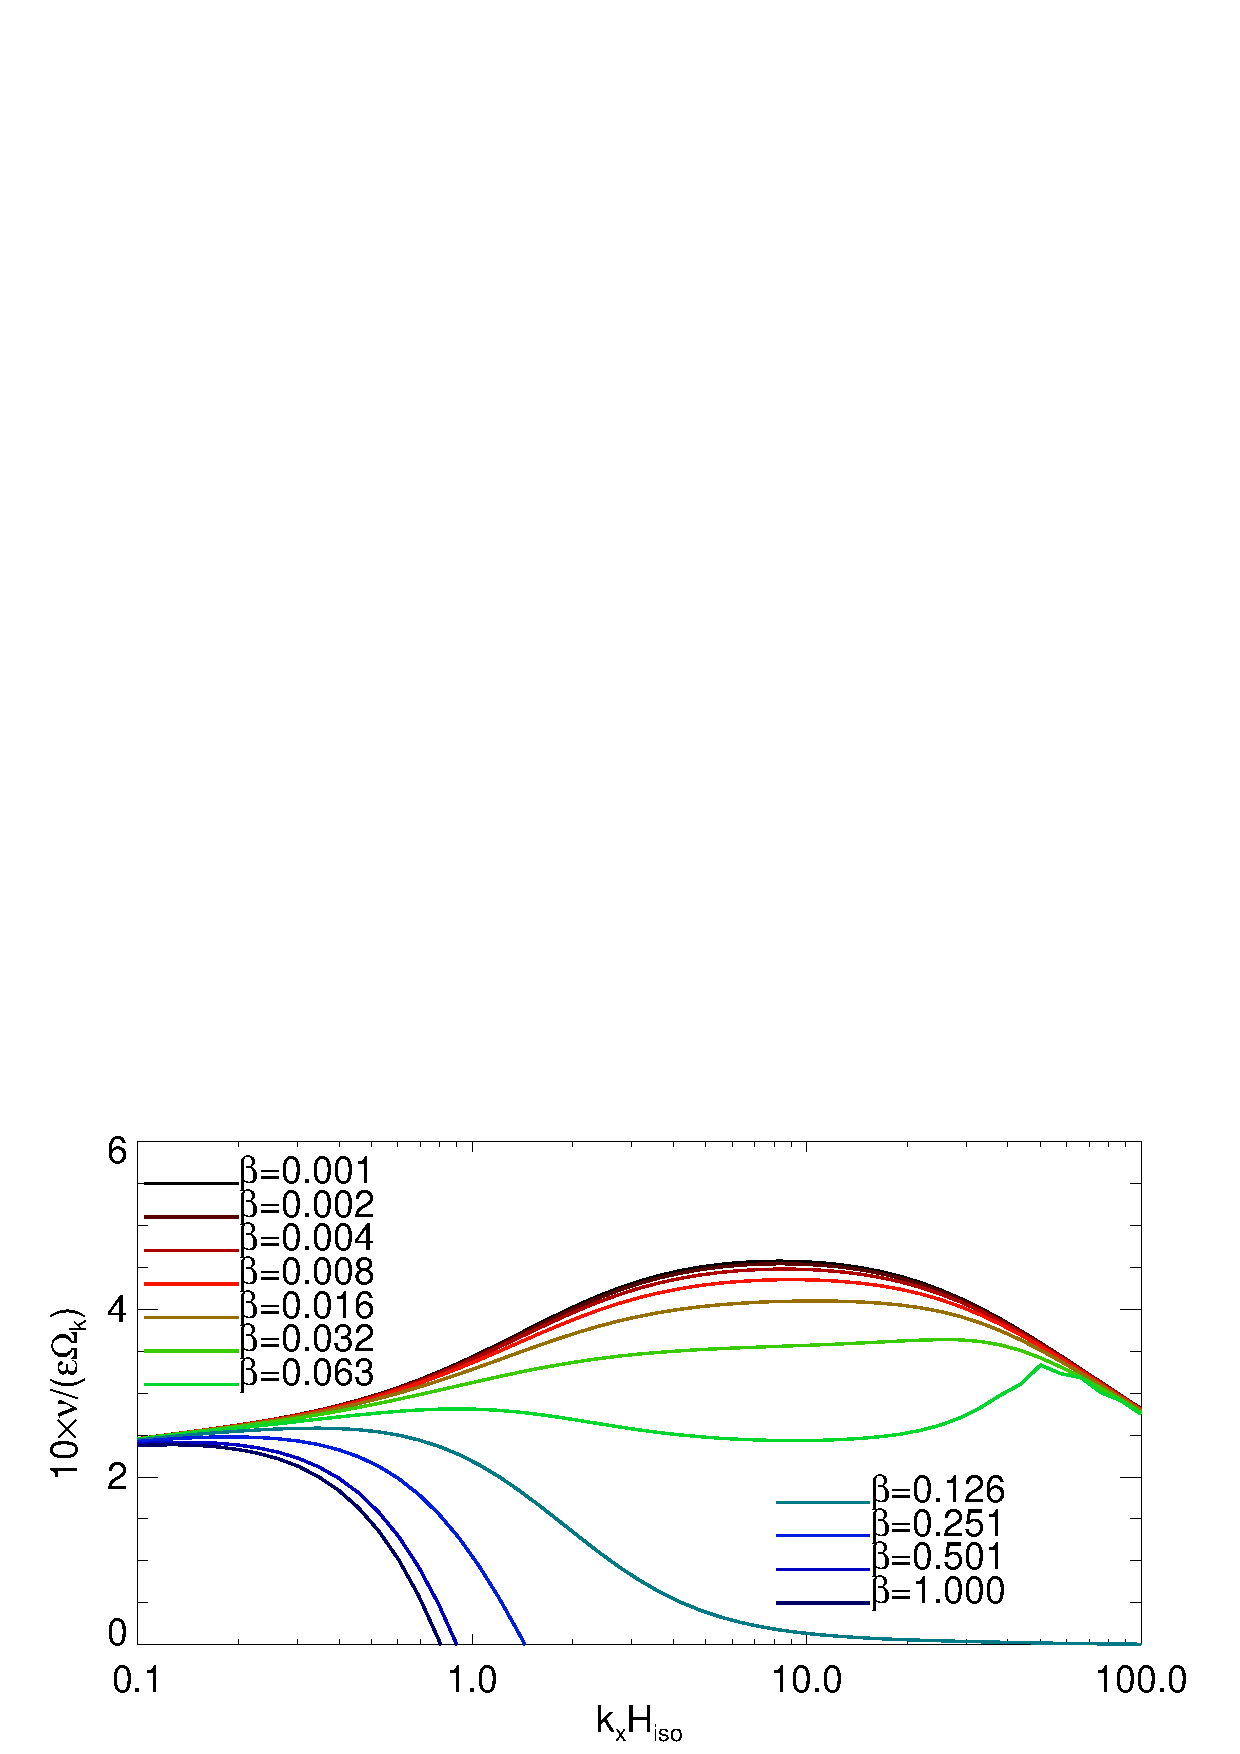
\includegraphics[width=\linewidth,clip=true,trim=0cm 0.0cm 0cm
%    0cm]{figures/compare_eigen_imag_bloop} 
%   % 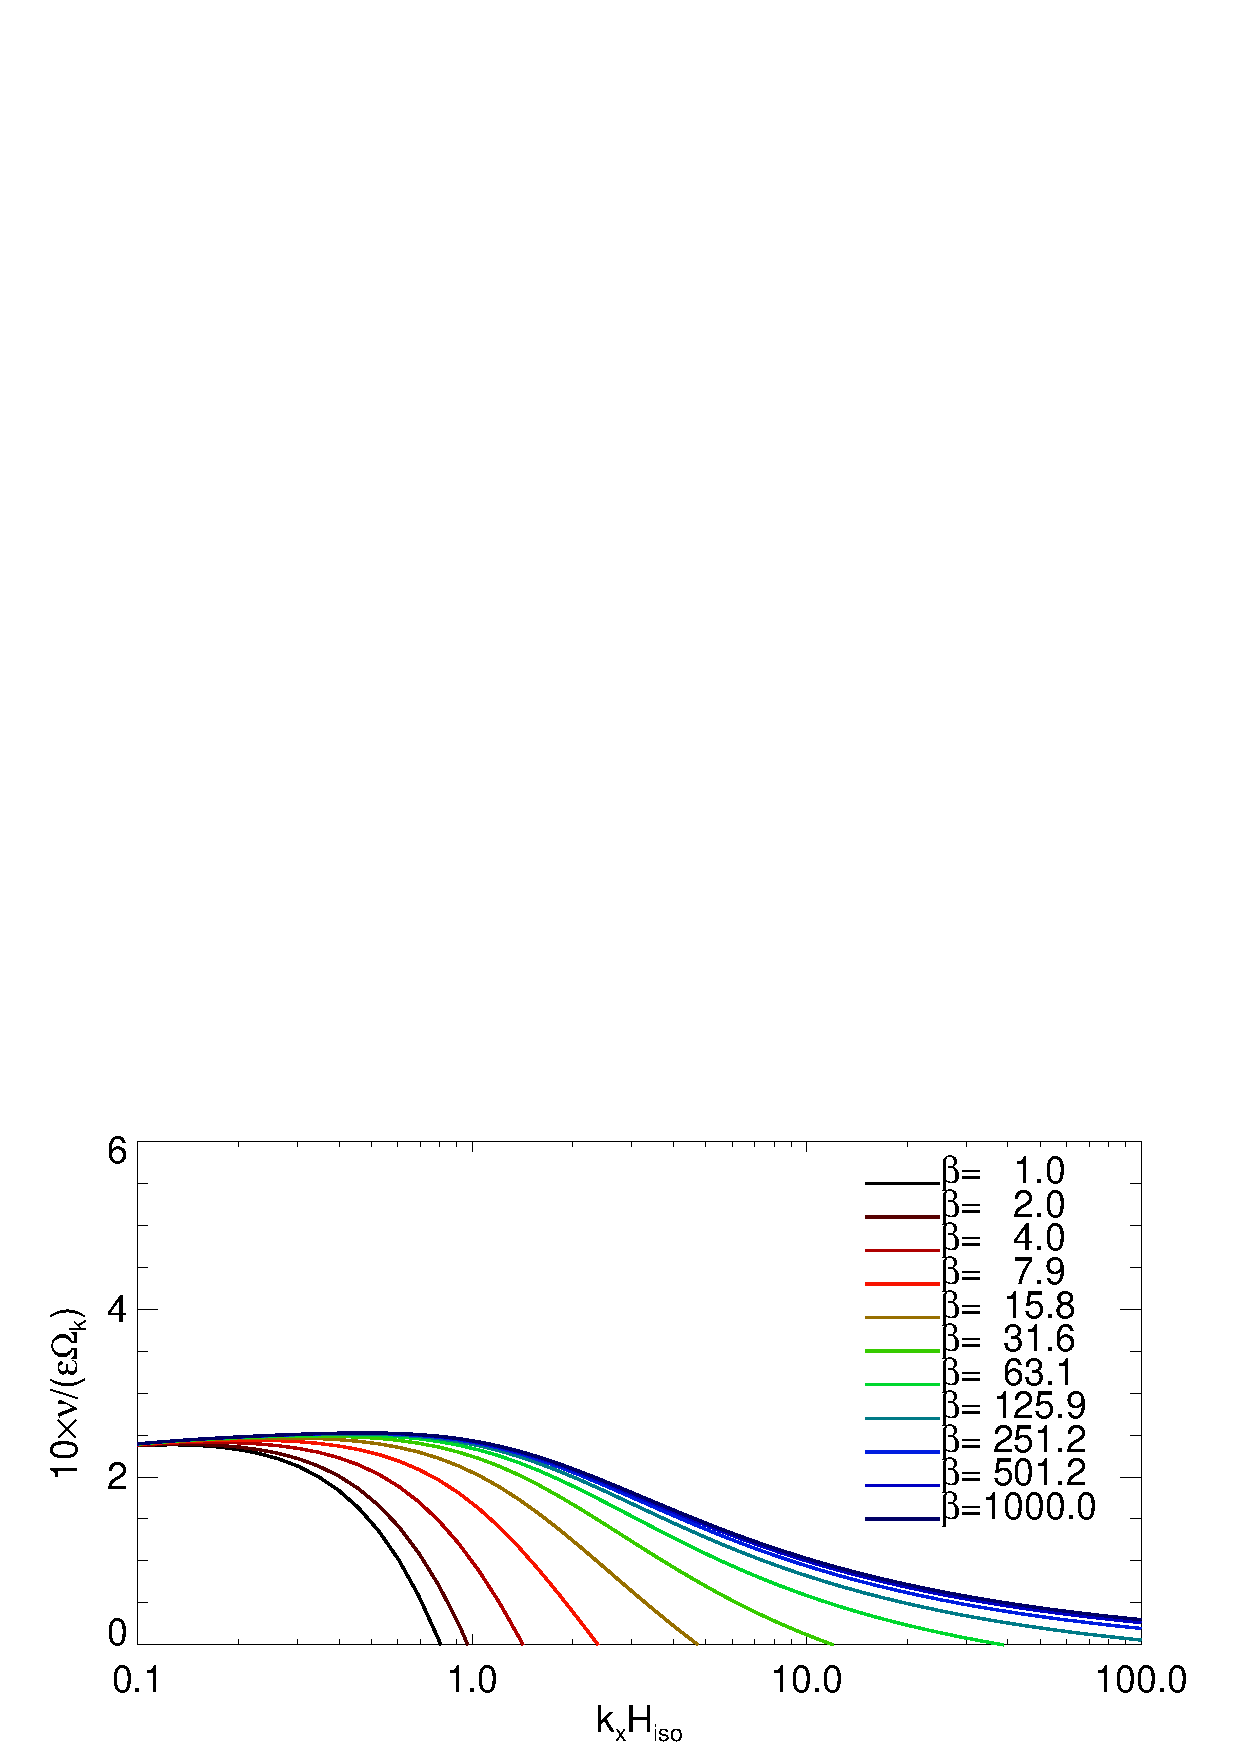
\includegraphics[width=\linewidth,clip=true,trim=0cm 0cm 0cm
%   % 1cm]{figures/compare_eigen_imag_bloop2} 
%   \caption{Growth rates of the fundamental VSI mode in 
%     nearly-vertically isothermal disks ($\Gamma=1.011$) with
%     $(p,q,\epsilon)=(-1.5,-1,0.05)$, evolved with $\gamma=1.4$ under a
%     range of thermal relaxation timescales   
%     $\beta$. The eigenfrequencies are calculated by numerically 
%     solving the full linear eigenvalue problem. \label{relax_growth_num}}   
% \end{figure} 


%approximately the perturbation wavenumber observed in the fiducial
%numerical simulation of \cite{nelson13}. 

We visualize the effect of thermal relaxation in 
Fig. \ref{relax_eigenW_num} by comparing the eigenfunction $W$ for
$\beta=0.01$ and $\beta=0.1$. The latter value is close to the
critical value beyond which the fundamental VSI is stabilized
(\S\ref{iso_vsi_beta_crit}). Increasing $\beta$ 
restricts  the region in which $W\sim z$ closer to the midplane, with
oscillatory behavior emerging at the boundaries, where buoyancy first
becomes important. Finite thermal relaxation increases $|W|$ near the
vertical boundaries relative to that about the midplane, but
perturbations near the disk surface is unlikely important in practice
because the disk atmosphere contains little mass. 

% We also find this trend for fixed $\beta$ but
% increasing 
% $\khat$.  

\begin{figure}
  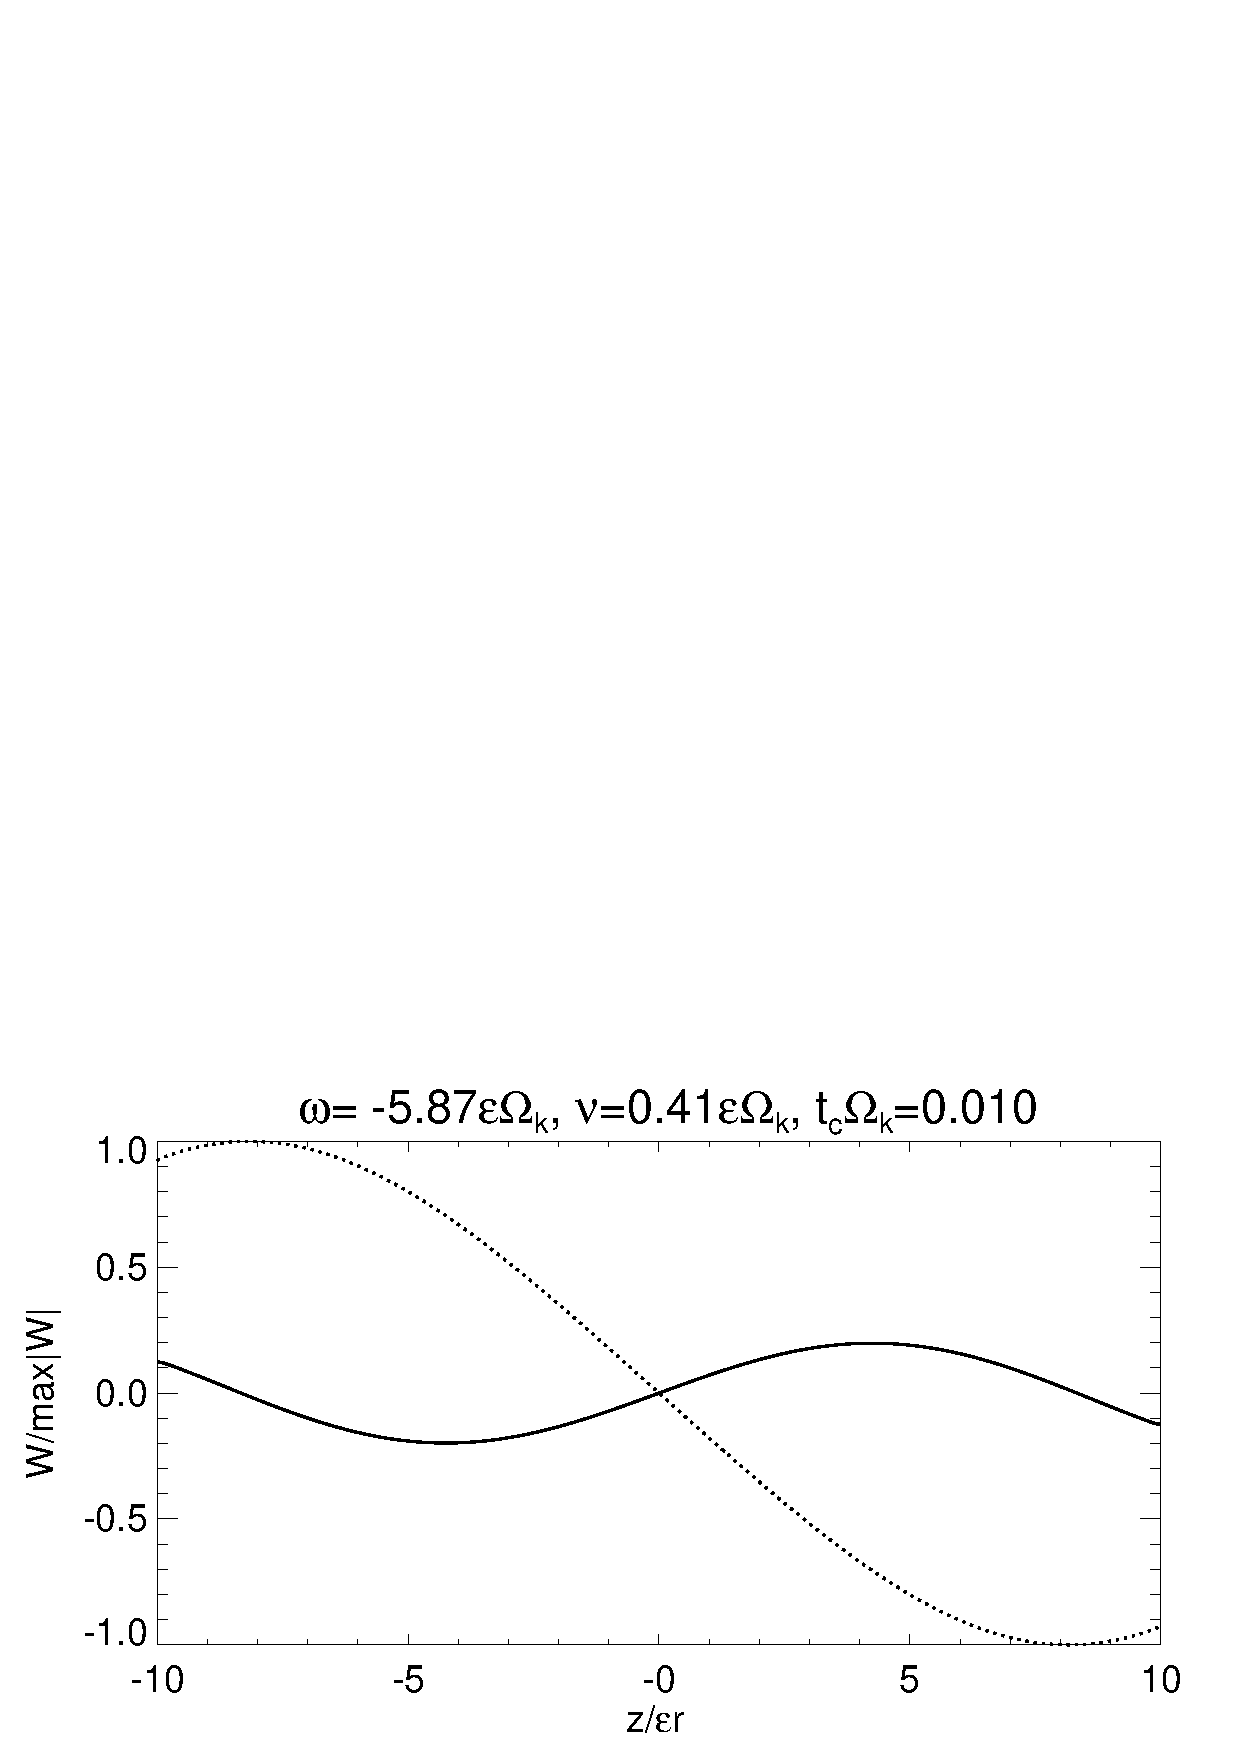
\includegraphics[width=\linewidth,clip=true,trim=0cm 1.75cm 0cm
  0cm]{figures/eigenvectorW_beta0d01} 
  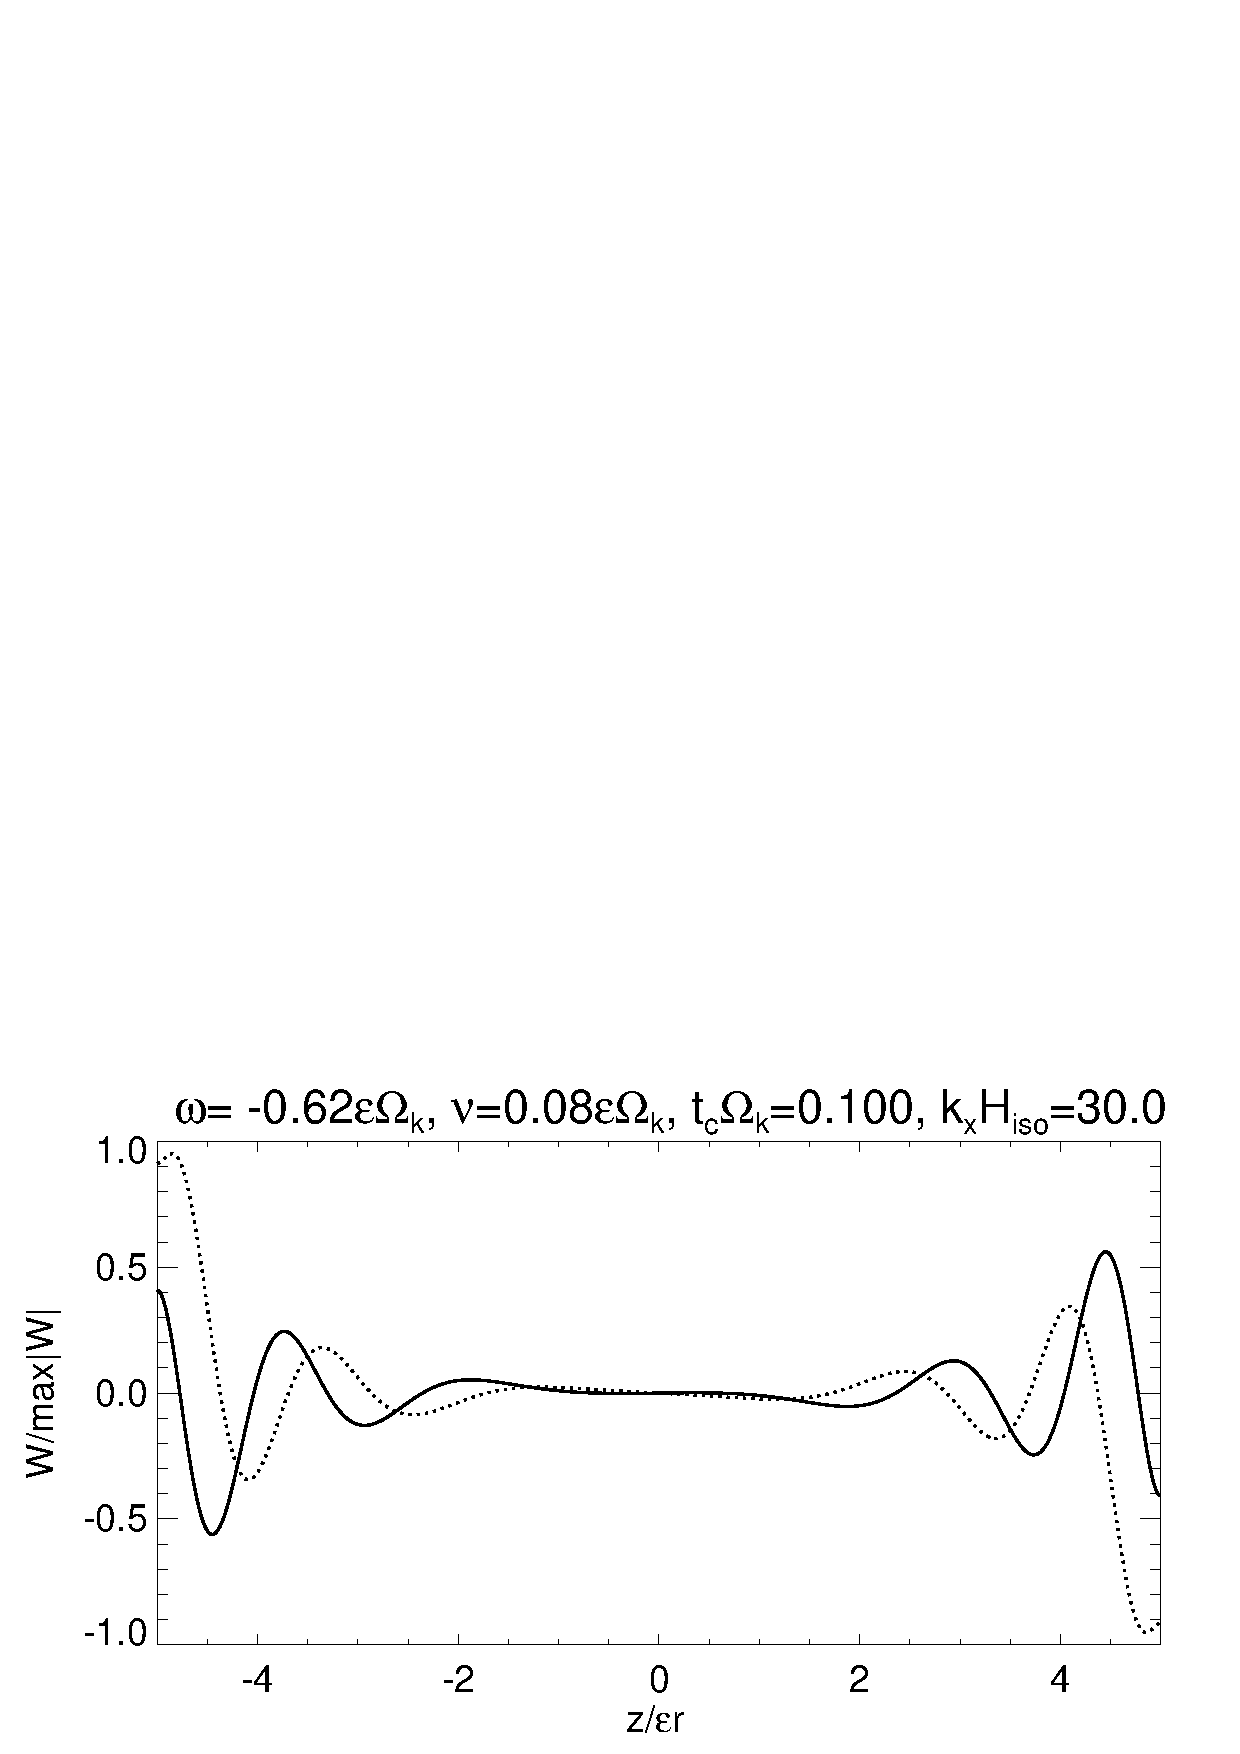
\includegraphics[width=\linewidth,clip=true,trim=0cm 0cm 0cm
  0cm]{figures/eigenvectorW_beta0d1} 
  \caption{Numerically-calculated eigenfunction of the fundamental VSI
    mode in a nearly vertically isothermal disk ($\Gamma=1.011$) with
    $(p,q,\epsilon)=(-1.5,-1,0.05)$, evolved with $\gamma=1.4$ and a dimensionless 
    thermal relaxation timescale $\beta = 0.01$
    (top) and $\beta=0.1$ (bottom). The
    perturbation radial wavenumber is $\khat=30$. The
    real (imaginary) part of $W$ is plotted as the solid (dotted)
    line.
    \label{relax_eigenW_num}}  
\end{figure}

\subsection{Critical thermal relaxation timescale}
% may need to explain why choose k=10
% bcrit independent of k for k>>1 
% for some parameter regimes (e.g. large q, large epsilon) 
% behavior at larger kx and finite bcool not understood. 
We test the dependence of the critical thermal relaxation timescale 
$\beta_\mathrm{crit}$ for the fundamental VSI on disk parameters
(Eq. \ref{iso_vsi_cond}).  We use the previous case study as a
reference point and vary $q\in[-0.2,-1.2]$, 
$\gamma\in[1.2,2.0]$, and $\epsilon\in[0.02,0.1]$
separately. Here, we use a wavenumber $\khat=10$, for which we
find growth rates reach zero for the range of disk parameters
considered, so that a numerical $\beta_\mathrm{crit}$ can be defined precisely. 

The numerically-obtained $\beta_\mathrm{crit}$ is shown in
Fig. \ref{bcrit_compare} in comparison with Eq. \ref{iso_vsi_cond}.
Our numerical results generally agree with Eq. \ref{iso_vsi_cond}. The
agreement improves with decreasing  $|q|$,  $\epsilon$ and increasing
$\gamma$, i.e. weaker instability, although there is a noticeable difference
as $\gamma\to1$ because the derivation of $\beta_\mathrm{crit}$
assumed $\gamma>1$.   

Fig. \ref{bcrit_compare}, together with the previous section
(Fig. \ref{bcrit_compare1}), shows that $\beta_\mathrm{crit}$ as given
by Eq. \ref{iso_vsi_cond} gives a measure of the characteristic
thermal timescale below which perturbations are effectively isothermal
so that the fundamental VSI operates. 

% From the previous section (Fig. \ref{relax_eigenW_num}) we
% expect that for other wavenumbers,  still gives a characteristic
% thermal timescale below which the perturbations are effectively
% isothermal. 


\begin{figure}
  \includegraphics[width=\linewidth,clip=true,trim=0cm 0.cm 0cm
  0cm]{figures/bcrit_compare_q.ps} 
  \includegraphics[width=\linewidth,clip=true,trim=0cm 0.0cm 0cm
  0.8cm]{figures/bcrit_compare_g.ps}
  \includegraphics[width=\linewidth,clip=true,trim=0cm 0.0cm 0cm
  0.8cm]{figures/bcrit_compare_e.ps} 
  \caption{Dependence of the upper limit to the thermal relaxation timescale
    $\beta_\mathrm{crit}$ for the fundamental VSI mode on disk
    parameters. The fiducial parameters are $\Gamma=1.011$,
    $\gamma=1.4$ and $(p,q,\epsilon)=(-1.5,-1,0.05)$. Top: varying
    $q\in[-1.2,-0.2]$; middle: varying $\gamma\in[1.2,2.0]$; bottom:
    varying $\epsilon\in[0.02,0.1]$. The perturbation wavenumber is
    $\khat=10$.  
    \label{bcrit_compare}}  
\end{figure}

\subsection{Vertically non-isothermal disks} 
We briefly consider vertically non-isothermal disks with 
$\Gamma=1.4$ and $(p,q,\epsilon)=(0,-1,0.05)$ as simulated in
\cite{nelson13}. In this case we set $\zmax\simeq2.2\epsilon r$, which
is close to the zero-density surface.      

Fig. \ref{gcorr_compare_vnoniso} plots the fundamental VSI growth
rates as a function of $\beta$ for $\gamma\in[1.4,2.5]$. For
comparison with \cite{nelson13} we consider 
$\beta\in[10^{-2},10^2]$. In agreement with \citeauthor{nelson13}, in
the neutrally-stratified case $\gamma=\Gamma$ the disk is unstable
even for $\beta\gg 1$. (Note that in the adiabatic limit
$\beta\to\infty$ this disk can be unstable according to the
Solberg-Hoiland criterion, Eq. \ref{solberg2}.) 

For $\gamma>\Gamma$, i.e. stably stratified disks,
Fig. \ref{gcorr_compare_vnoniso} shows that introducing finite thermal
relaxation rapidly stabilizes the fundamental VSI mode. This is
similar to that observed for nearly vertically isothermal disks
(Fig. \ref{bcrit_compare1}). For $\gamma=1.7,\,2.0,\,2.5$, growth
rates reach zero for  $\beta\simeq0.17,\,0.083,\,0.045$, respectively.
Interestingly, these values are equal to
$\epsilon|q|/(\gamma-\Gamma)$. This suggests that the critial thermal
relaxation timescale for vertically non-isothermal disks can also be
estimated by Eq. \ref{iso_vsi_cond} but with $\gamma-1$ replaced by
$\gamma-\Gamma$. 

\begin{figure}
  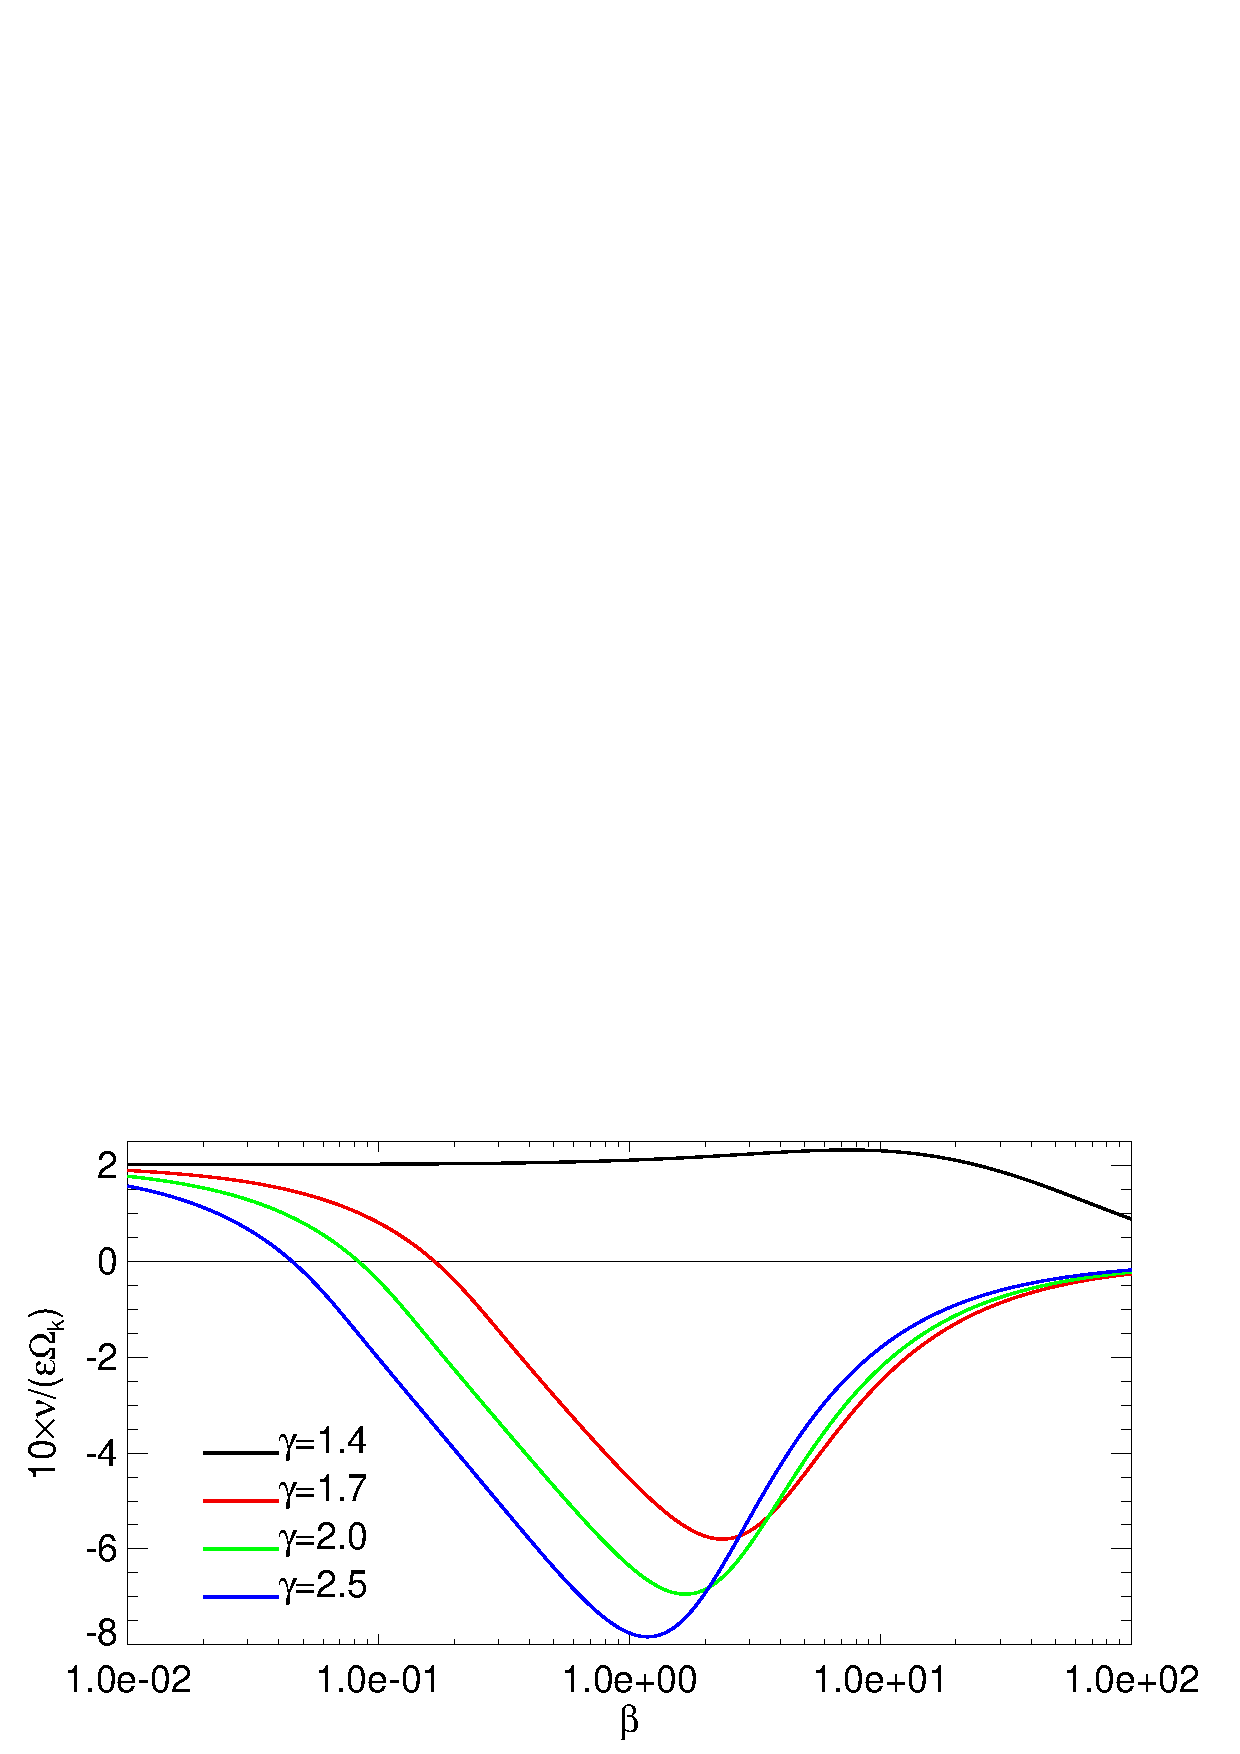
\includegraphics[width=\linewidth,clip=true,trim=0cm 0cm 0cm
  0cm]{figures/gcorr_compare_vnoniso}
  \caption{Growth rate of the fundamental VSI mode as a function of
    the thermal relaxation timescale $\beta$, in vertically
    non-isothermal disks with $\Gamma=1.4$ and
    $\gamma\in[1.4,2.5]$. The disk is neutrally
    stratified for $\gamma=1.4$ and stably stratified for
    $\gamma>1.4$. Other disk parameters are
    $(p,q,\epsilon)=(0,-1,0.05)$ and the perturbation wavenumber is
    $\khat=30$.  
    \label{gcorr_compare_vnoniso}}
\end{figure}












% \subsection{VSI in a stably stratified disk}
% We demonstrate the (strong) stabilizing effect of a  
% positive vertical entropy gradient ($N_z^2\geq0$) by setting $\gamma=2$.  
% Since we expect the perturbations to decay rapidly
% away from the midplane (see \S\ref{analytic_adia}), we consider a
% smaller domain with $\zmax = 2\epsilon r$. 
% Other disk and perturbation parameters are the same as in
% \S\ref{vertiso_pertiso}.    

% Fig. \ref{lowfreq_eigen_adia} show the eigenvalues for this
% problem. The growth rates are much smaller than
% those in the previous section. The fundamental VSI mode is that with
% $\mathrm{max}\nu$. Its expected and numerically-calculated growth
% rates compares well, with 
% \begin{align*}
%   \nu = 0.03751 \epsilon \Omega_k &\quad \text{(from
%     Eq. \ref{gam2_growth_rate})},\\
%   \nu = 0.03672 \epsilon \Omega_k &\quad \text{(numerical)}.
% \end{align*}
% The fundamental mode is plotted in Fig. \ref{lowfreq_eigenfunc_adia},
% and clearly show that perturbations are rapidly stabilized away from
% the midplane. For the adopted disk and perturbation parameters,
% Eq. \ref{gam2_alpha} gives $\real{\alpha}\simeq - 43.8$, corresponding
% to a characteristic decay length scale of $\sqrt{2/|\alpha|}\epsilon r\simeq 0.2\epsilon r$,
% which is consistent with that observed in  Fig. \ref{lowfreq_eigenfunc_adia}. 

% This decay lengthscale is rougly the height within which
% vertical shear is larger than the buoyancy frequency squared. That is,
% \begin{align*}
% \left|r\frac{d\Omega^2}{dz}\right|\gtrsim N_z^2
% \end{align*}
% for
% \begin{align*}
%   \left|\frac{z}{\epsilon r}\right| \lesssim \frac{\epsilon|q|\gamma}{\gamma-1},
% \end{align*}
% in a thin, vertically isothermal disk. This evaluates to $|z|\lesssim
% 0.2\epsilon r$ for the current disk model, consistent with
% Fig. \ref{lowfreq_eigenfunc_adia}. 

% Furthermore, the growth rate to should be no larger than the
% maximum vertical shear available within this decay lengthscale. Using 
% Eq. \ref{max_growth} as a rough guide, 
% \begin{align}
%   \frac{\nu}{\epsilon\Omega_k}<\frac{\epsilon |q|^2\gamma}{2(\gamma-1)},
% \end{align}
% or $\nu< 0.1\epsilon\Omega_k$ in our disk model,
% consistent with numerical results. 

% \begin{figure}
%   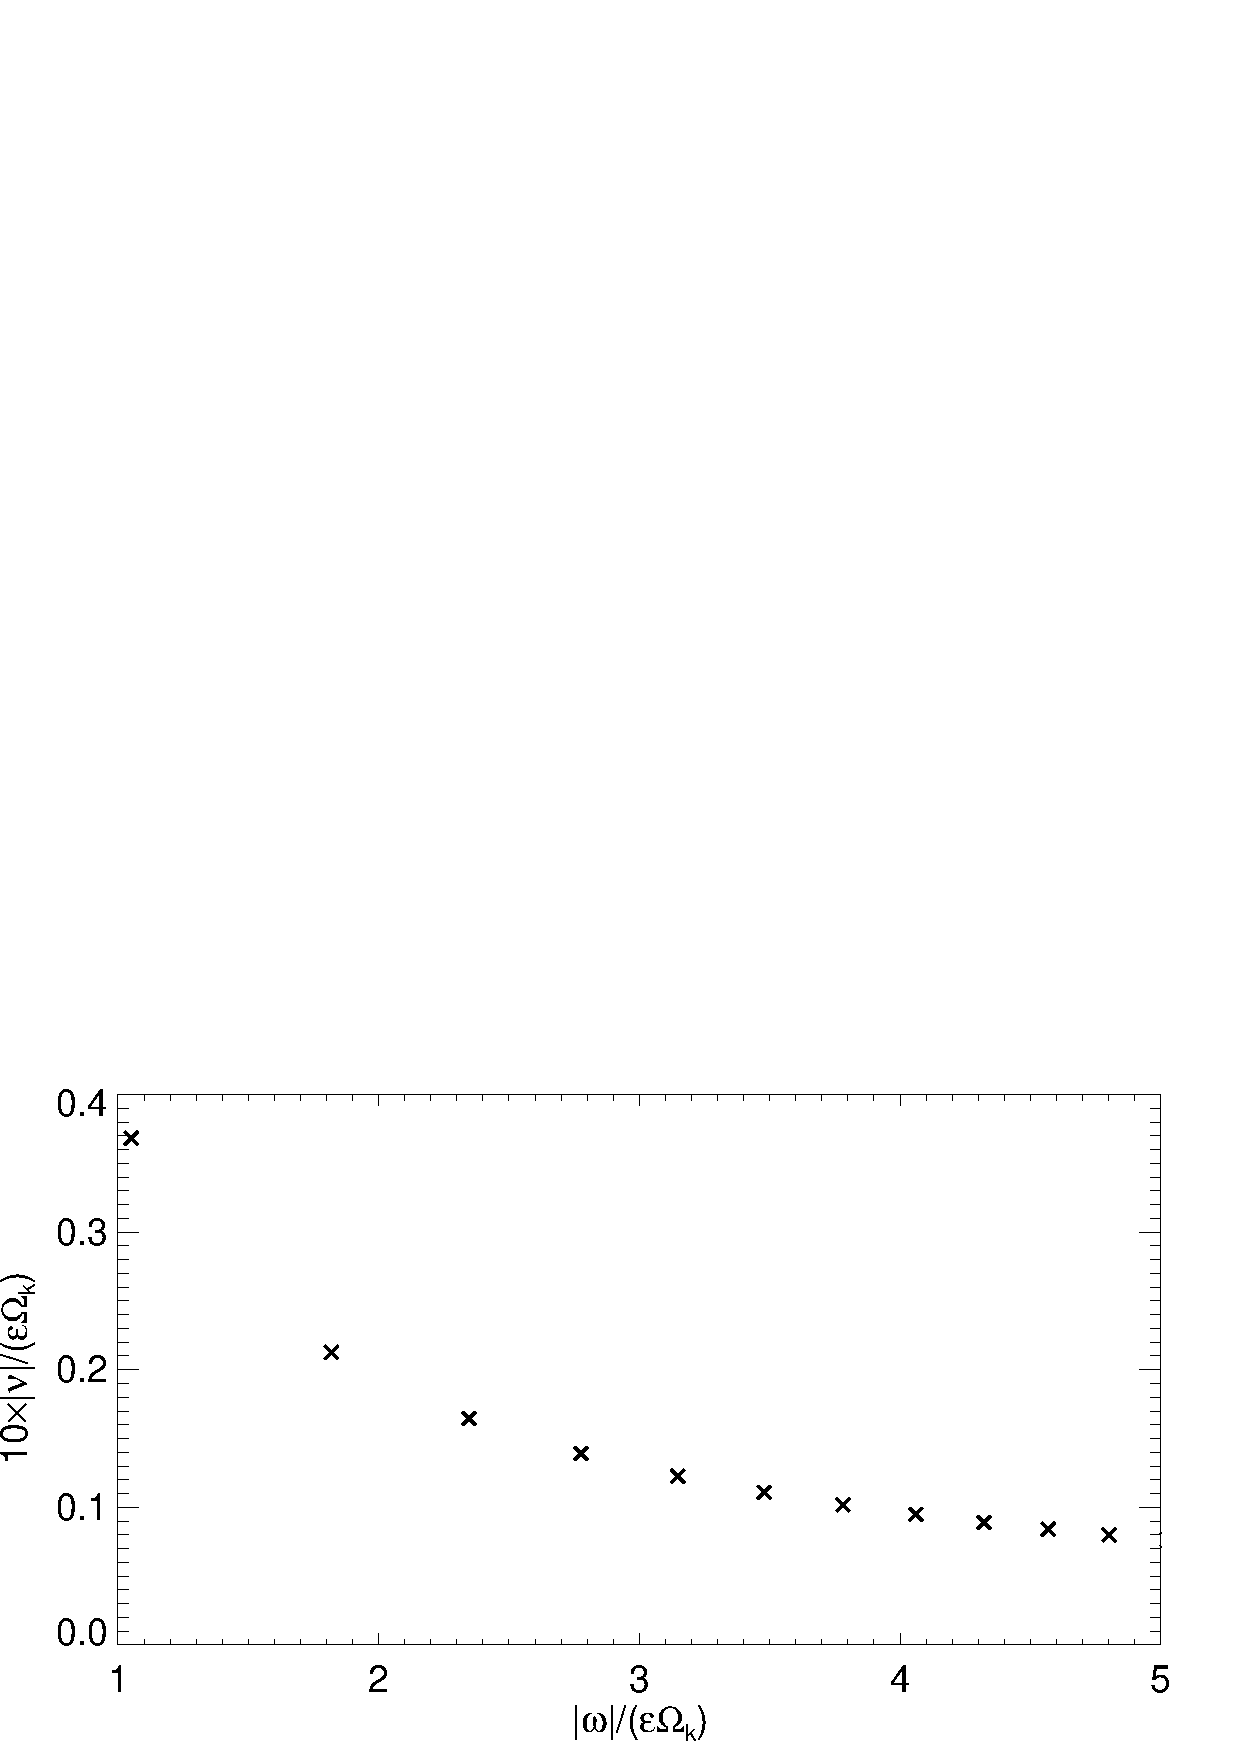
\includegraphics[width=\linewidth]{figures/eigenvalues_adia}
%   \caption{Eigenvalues in for the
%     VSI in a nearly vertically isothermal disk
%     ($\Gamma=1.011$) with $(p,q,\epsilon)=(-1.5,-1,0.1)$, 
%     evolved adiabatically with $\gamma=2$. The perturbation radial
%     wavenumber is $\khat=20\pi$. \label{lowfreq_eigen_adia}
%   }
% \end{figure}
  

% \begin{figure}
%   \includegraphics[width=\linewidth]{figures/eigenvectorvz_adia}
%   \caption{Fundamental VSI mode in a nearly vertically
%     isothermal disk ($\Gamma=1.011$) with $(p,q,\epsilon)=(-1.5,-1,0.1)$, 
%     evolved adiabatically
%     with $\gamma=2$. This eigenfunction 
%     corresponds to the top-left eigenvalue displayed in 
%     Fig. \ref{lowfreq_eigen_adia} (largest $|\nu|$).  
%     The  real (imaginary) part of $\delta v_z$ are shown as solid
%     (dotted) lines. 
%     \label{lowfreq_eigenfunc_adia}
%   }
% \end{figure}

% Although a positive vertical entropy gradient is stabilizing, we note
% that $N_z^2\propto z^2$  while vertical shear $rd\Omega^2/dz\propto
% z$, so that there is always a region sufficiently close to the
% midplane in which vertical shear dominates over bouyancy and the VSI
% can operate. However, the growth rates are small and the instability
% only affects the regions close the midplane. These modes may not be
% important in practice.  


% \subsection{Other adiabatic indices}
% To see the transition from neutrally-bouyant to stably stratified cases above, 
% we repeated the previous calculation with $\gamma\in[1,2]$. 
% We restore the vertical domain to $\zmax=10\epsilon r$. 
% Fig. \ref{adia_growth_num} shows the eigenfrequencies of the
% fundamental VSI mode. 


% %To select the appropriate
% %eigenvalues we vary the parameters slowly away from a reference solution.   
% % The numerically-determined eigenfrequencies are qualitatively
% % consistent with the discussion in \S\ref{adia_compare_gam1}.
% There is good agreement between Fig. \ref{adia_growth_num} and
% Fig. \ref{adia_growth} for $\khat=k_xH_\mathrm{iso}\gtrsim1$. There is a
% mismatch for smaller wavenumbers, especially in the growth
% rates. Actual growth rates decrease slower as $\khat\to0$
% than that in Fig. \ref{adia_growth}. Disagreement at small
% $\khat$ is not unexpected because the low-frequency
% approximation used to obtain Fig. \ref{adia_growth} becomes invalid since
% $|\omega|\sim\Omega_k$ for small $\khat$.  

% Given the number of approximations made in \S\ref{adia_compare_gam1},
% Fig. \ref{adia_growth_num} compares well with 
% Fig. \ref{adia_growth}. The main qualitative features of the full
% numerical solution in Fig. \ref{adia_growth_num} are captured by
% Fig. \ref{adia_growth}: stabilization for 
% $\khat\to0$ and $\khat\to\infty$,
% stabilization for increasing $\gamma$ (but ineffective at small $\khat$), 
% and the shift of the most unstable wavenumber to smaller values as
% $\gamma$ is increased. 


% \begin{figure}
%   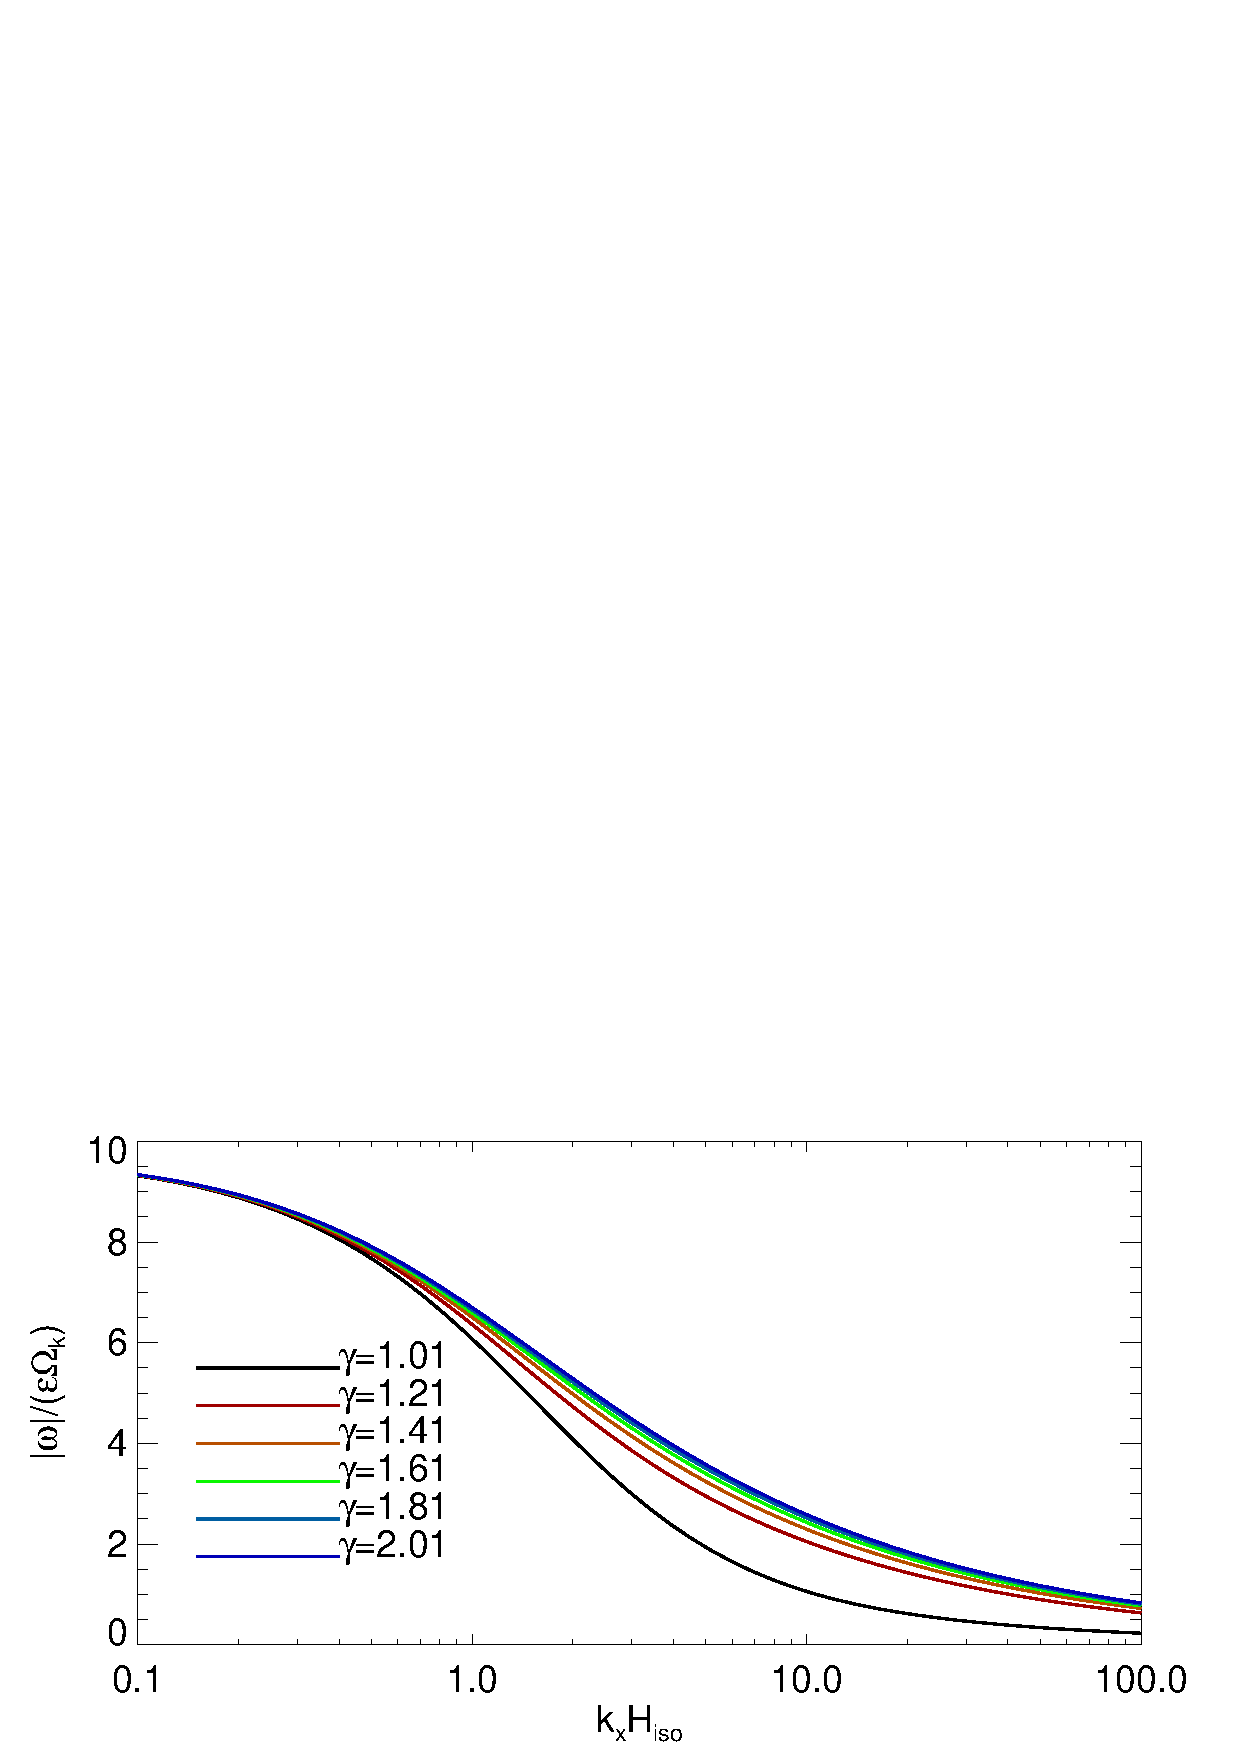
\includegraphics[width=\linewidth,clip=true,trim=0cm 1.75cm 0cm 0cm]{figures/compare_eigen_real1}
%   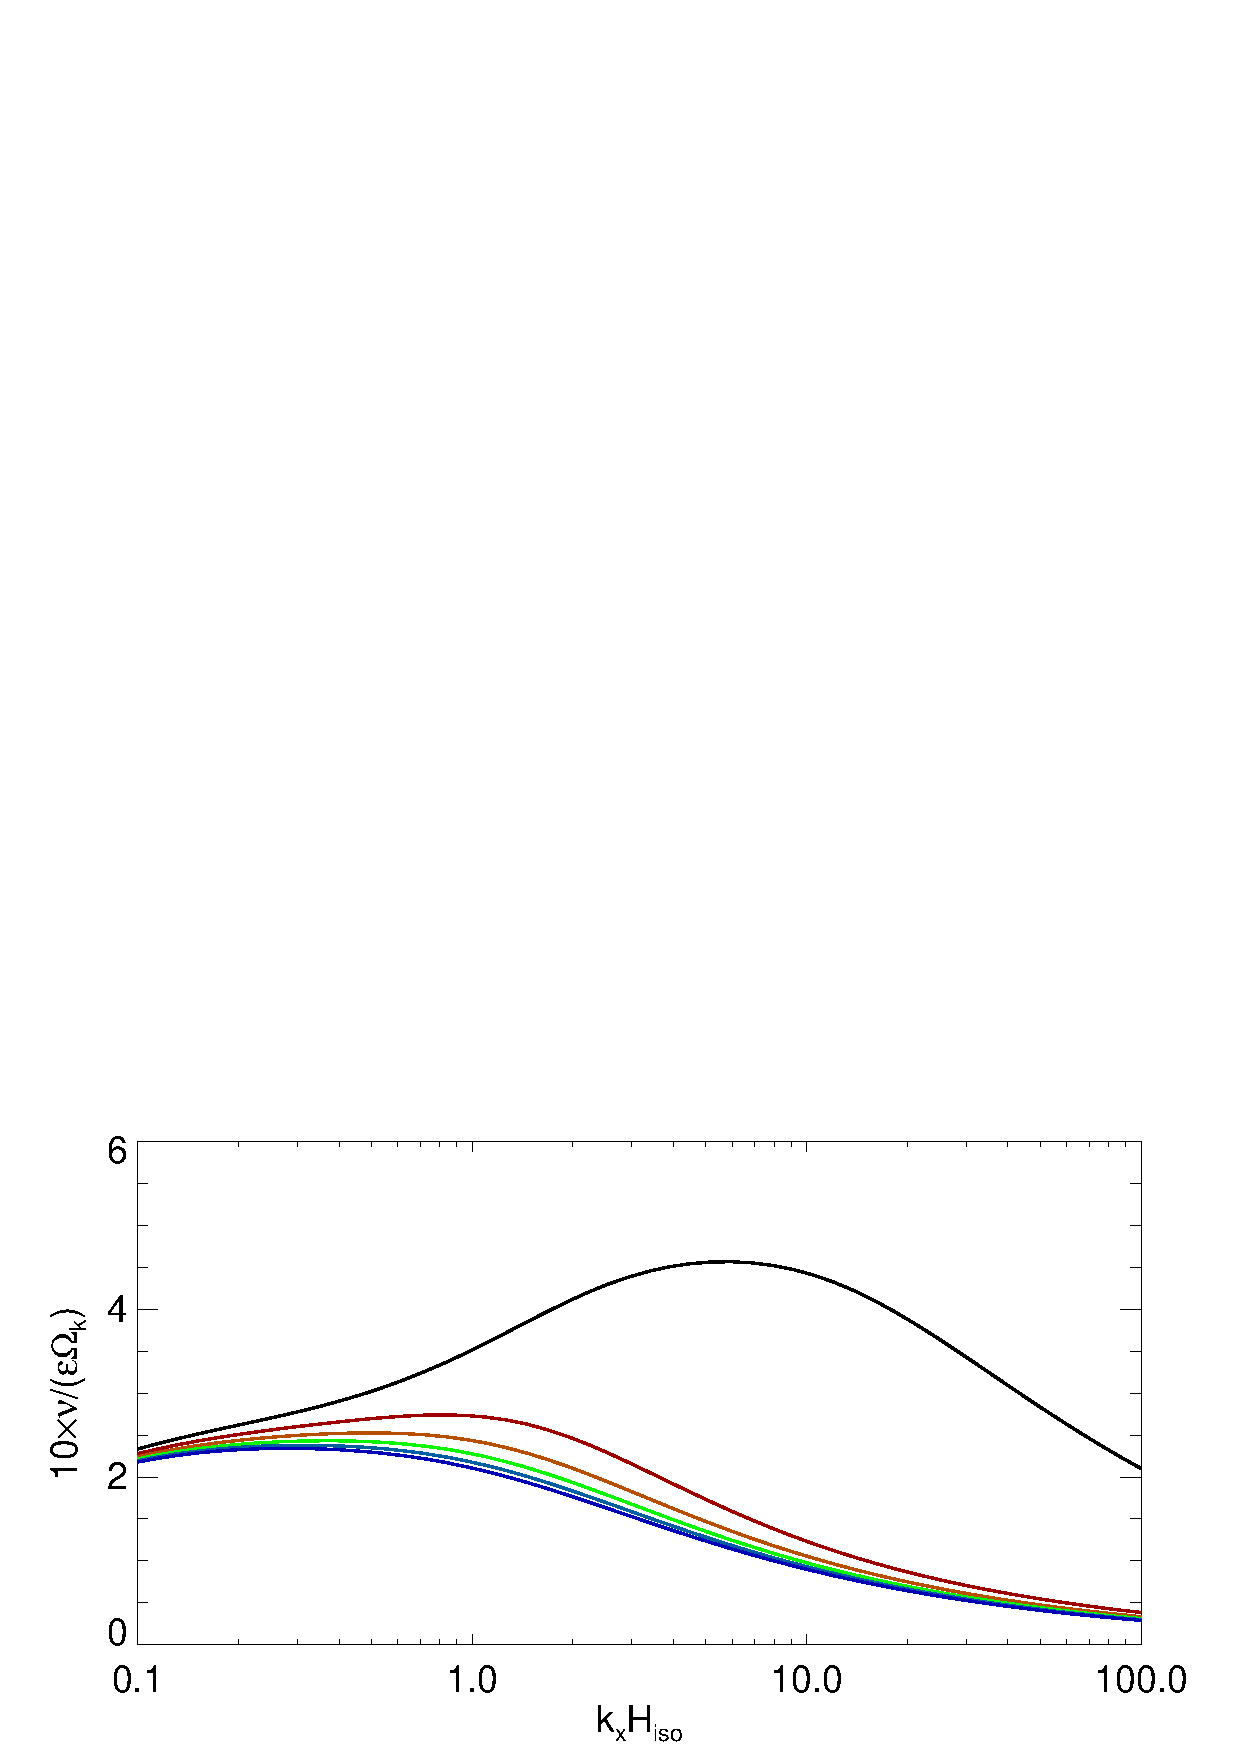
\includegraphics[width=\linewidth,clip=true,trim=0cm 0cm 0cm 1cm]{figures/compare_eigen_imag1}
%   \caption{Real frequency (top) and growth rate 
%     (bottom) of the fundamental VSI in a nearly vertically   
%     isothermal disks ($\Gamma=1.011$) with $(p,q,\epsilon)=(-1.5,-1,0.1)$, 
%     subject to adiabatic perturbations with different values of $\gamma$. 
%     The eigenfrequencies are calculated by numerically
%     solving the full linear eigenvalue problem. This plot is to
%     be compared with Fig. \ref{adia_growth}. \label{adia_growth_num}}   
% \end{figure}  

\section{Application to protoplanetary disks}\label{application} 
As an application of our linear models, we estimate where in a
protoplanetary disk do the thermodynamic conditions allow the VSI to
operate. For a realistic disk one can consider the energy equation
with radiative cooling, 
\begin{align}\label{real_energy}
  % \rho T \frac{DS}{Dt} = - \left(\nabla\cdot\bm{F} - Q_+\right), 
  \frac{\p P}{\p t} + \bm{v}\cdot\nabla P +\gamma P \nabla\cdot\bm{v} = - \frac{P}{\rho T
    c_v}\left(\nabla\cdot\bm{F} - Q_+\right), 
\end{align}
where $c_v$ is the heat capacity at constant
volume, 
$\bm{F}$ is the radiative flux and $Q_+$ is a heating
term to permit an equilibrium solution. 

One should now model in detail each of the terms on the RHS of
Eq. \ref{real_energy}, linearize them, then solve 
the resulting linear eigenvalue problem. This is beyond 
the scope of the present work. Here, we take the simpler approach of
modeling the linearized RHS of Eq. \ref{real_energy} such that it can 
be represented by a thermal relaxation time $t_c$. 
To do so, we first consider separately perturbations
with radial lengthscales $l\gg l_\mathrm{rad}$ and  
$l\ll l_\mathrm{rad}$, where      
\begin{align}\label{lrad}
  l_\mathrm{rad} \equiv \frac{1}{\kappa_d\rho} 
\end{align} 
is the photon mean-free-path and $\kappa_d$ is the (dust) opacity. 

\subsection{Radiative diffusion}
For perturbations with lengthscales $l\gg
l_\mathrm{rad}$, we assume temperature fluctuations are smoothed out
by radiative diffusion and model this in linear theory by writing the
linearized RHS of Eq. \ref{real_energy} as 

\begin{align}\label{diff_cool_proper}
  \frac{P}{\rho T c_v} \nabla\cdot\left(k_\mathrm{rad}\nabla\delta
    T\right),  
\end{align}
where $k_\mathrm{rad}$ is the conduction coefficient to be defined
implicitly. 

However, Eq. \ref{diff_cool_proper} fundamentally changes the linear
problem by introducing higher order derivatives. We defer a proper
analysis of this problem to a follow-up study. Here, we are interested
in order-of-magnitude estimates for perturbations with radial
lengthscales much smaller than vertical lengthscales. We thus proceed 
by assuming vertical derivatives can be neglected in 
Eq. \ref{diff_cool_proper} and write  
\begin{align}\label{diff_cool_approx}
  \frac{P}{\rho T c_v} \nabla\cdot\left(k_\mathrm{rad}\nabla\delta
    T\right) &\to -\frac{k_\mathrm{rad}}{\rho
    c_v}k_x^2P\left(\frac{\delta T}{T}\right)\notag\\
  &\equiv -\eta k_x^2 \left(\delta P - \frac{P}{\rho}\delta\rho\right), 
\end{align}
where $\eta=k_\mathrm{rad}/\rho c_v$ is the diffusion coefficient and
is given in terms of physical disk parameters as 
\begin{align}\label{eta_def}
  \eta = \frac{16\sigma_s T^3}{3\kappa_d\rho^2 c_v}, 
\end{align}
where $\sigma_s$ is the Stefan-Boltzmann constant. 
From Eq. \ref{diff_cool_approx} we identify the scale-dependent thermal relaxation
time for diffusion as 
\begin{align}\label{tc_diff_cool} 
  t_\mathrm{diff} = \frac{1}{\eta k_x^2}.%\equiv \frac{\Omega_k^{-1}}{\hat{\eta}\khat^2}, 
\end{align}

\subsection{Newtonian cooling}\label{newton_cool}
For perturbations with small lengthscales, $l\ll l_\mathrm{rad}$, 
the disk is optically thin. In this case, we assume 
Newtonian cooling can be applied, which is the thermal
relaxation model as adopted in our linear models. That is, temperature
fluctuations $\delta T$ decay on a timescale $t_\mathrm{cool}$,
independent of $k_x$. For simplicity, we take  
\begin{align}
  t_\mathrm{cool} = \frac{l_\mathrm{rad}^2}{3\eta}. 
\end{align}
We note that $t_\mathrm{cool}$ does not explicitly depend on $\rho$. 

\subsection{A model for combined thermal relaxation}\label{toy_relax}
To unify $t_\mathrm{cool}$ and $t_\mathrm{diff}$, we define the
effective thermal relaxation timescale in linear theory as
\begin{align}\label{tc_def}
  t_c &\equiv t_\mathrm{cool} + t _\mathrm{diff}. %=
  % \frac{l_\mathrm{rad}^2}{3\eta} + \frac{1}{\eta k_x^2},  
\end{align}
Eq. \ref{tc_def} is a simple prescription so
that for small scales (large $k_x$), $t_c\to t_\mathrm{cool}$, while
for large scales (small $k_x$), $t_c\to t_\mathrm{diff}$. Writing the
volume density $\rho = \Sigma\hat{\rho}/\sqrt{2\pi}H$, where
$\hat{\rho} = \rho/\rho_0$ and $\Sigma$ is the surface density at the
radius of interest, the dimensionless thermal
relaxation time $\beta$ becomes 
\begin{align}\label{real_beta}
  \beta(z;\khat) \equiv t_c\Omega_k =
  % \frac{1}{\hat{\eta}}\left[\frac{l_\mathrm{rad}^2}{3H^2}
  %   + \frac{\hat{\rho}^2(z)}{2\pi\khat^2}\right]  \simeq
  \frac{\Sigma^2\Omega_k}{\eta\rho^2}\left[\frac{1}{3\kappa_d^2\Sigma^2} 
    + \frac{\hat{\rho}^2(z)}{2\pi \khat^2}\right].
\end{align}
Note that $\beta$ depends on both the perturbation lengthscale $\khat$ 
and distance from the midplane. 

\subsection{Evaluation for a fiducial disk model}
We evaluate Eq. \ref{real_beta} for the protoplanetary disk model
described in \cite{chiang10} and summarized in Appendix \ref{mmsn}
(where an opacity model is also chosen). Defining $r_\mathrm{AU}\equiv 
r/\mathrm{AU}$, we find Eq. \ref{real_beta} becomes
\begin{align}\label{beta_mmsn}
  \beta(z; \khat) =
  &\frac{4.4\times10^5}{\mu(\gamma-1)}\left(\frac{\hat{\kappa}_d\hat{\Sigma}^2}{\hat{T}}\right)r_\mathrm{AU}^{-57/14}\notag\\ 
&\times\left[\frac{8.3\times10^{-9}}{\hat{\kappa}_d^2\hat{T}^4\hat{\Sigma}^2}r_\mathrm{AU}^{33/7}+\frac{\hat{\rho}^2(z)}{2\pi\khat^2}\right].         
\end{align} 
We refer to the case with $\gamma=1.4$, $\mu=2.33$ and the scalings
$\hat{\Sigma}=\hat{\kappa}_d=\hat{T}=1$ as the Minimum Mass Solar
Nebulae (MMSN) and $\beta=\beta_\mathrm{MMSN}$, 
\begin{align}\label{beta_mmsn_simp}
  \beta_\mathrm{MMSN} = 3.9\times10^{-3} r_\mathrm{AU}^{9/14}\left( 1 +
    1.9\times10^7\hat{\rho}^2r_\mathrm{AU}^{-33/7}\khat^{-2}\right). 
\end{align}
% where
% \begin{align}
%   \
% %  \frac{3.7\times10^{-3}}{\mu\left(\gamma-1\right)\hat{\kappa}_d\hat{T}^5}, 
% \end{align}
% and
% \begin{align}
%   \khat_0 = 4.4\times10^{3}\hat{\kappa}_d\hat{T}^2\hat{\Sigma}.
% \end{align}
It is instructive to compare the above thermal timescale 
with the criterion Eq. \ref{iso_vsi_cond} evaluated for the MMSN,     
\begin{align}\label{bcrit_mmsn}
  % \beta_\mathrm{crit} = \frac{1.44\times10^{-2}}{(\gamma
  % -1)}\left(\frac{\hat{T}}{\mu}\right)^{1/2}r_\mathrm{AU}^{2/7}. 
  \beta_\mathrm{crit,MMSN} = 0.024r_\mathrm{AU}^{2/7}. 
\end{align}

In Fig. \ref{mmsn_bcrit_bcool} we plot Eq. \ref{beta_mmsn}  with $\mu
=2.33$ $\gamma=1.4$, $\hat{T}=\hat{\Sigma}=1$ for opacity scales
$\hat{\kappa}_d=0.1, \,1 $ (MMSN) and $10$, at $z=0$ and $z=3H$. We
also plot Eq. \ref{bcrit_mmsn} in each panel.   

Consider first the MMSN shown in the middle panels of 
Fig. \ref{mmsn_bcrit_bcool}. The critical thermal timescale,
Eq. \ref{bcrit_mmsn}, is useful in the optically thin regime (where the
curves overlap), since in this limit $\beta$ does not depend on
height, as assumed in our analysis. We thus infer that the VSI can
operate at tens of AU in the MMSN.  

In the inner few AU of the MMSN, however, $\beta$ 
may be smaller or greater than $\beta_\mathrm{crit}$ depending on
$z$ as the disk transitions from an optically thick midplane to an
optically thin atmosphere. 
%Given a fixed $\khat$, one can have $\beta > \beta_\mathrm{crit}$ at
%the optically thick midplane, but with increasing height the disk 
%becomes optically thin and $\beta<\beta_\mathrm{crit}$. 
Our analytical criteria is not valid for variable $\beta$, and we must
turn to numerical solutions of the linear problem to determine whether
or not the VSI operates. We do this in the next section.   
 
Lowering the opacity, as shown in the top panels of
Fig. \ref{mmsn_bcrit_bcool}, shifts the curves inwards but also raises
them. In fact, lowering the opacity by an order of magnitude renders  
$\beta > \beta_\mathrm{crit}$ even away from the midplane. This is 
expected to stabilize the disk. Raising the opacity, as shown in 
the lower panels of Fig. \ref{mmsn_bcrit_bcool}, decreases the thermal
timescales, but shifts the curves outward, so the instability is
restricted to larger radii.  

\begin{figure*}
  \includegraphics[scale=.47,clip=true,trim=0cm 1.8cm 0cm
  0cm]{figures/bcrit_mmsn_kap0d1_z0}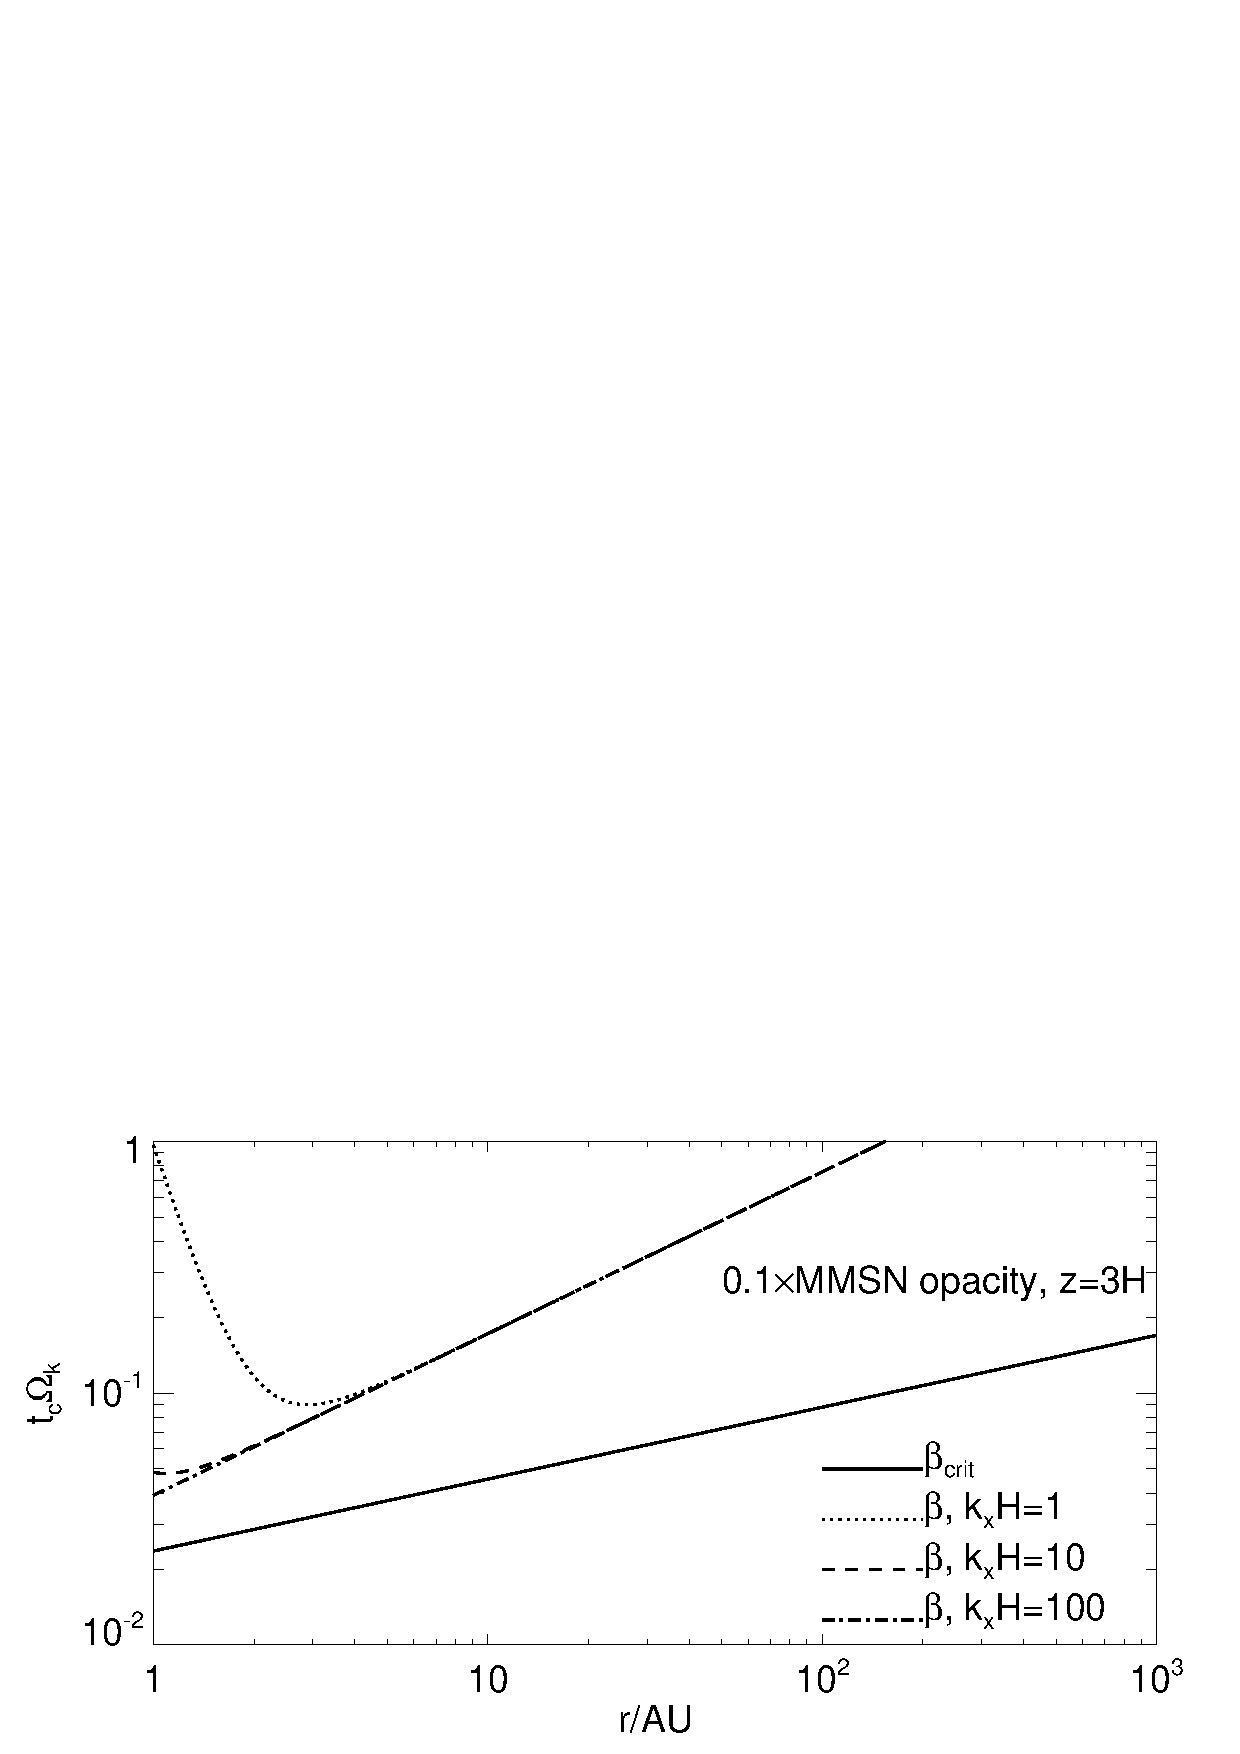
\includegraphics[scale=.47,clip=true,trim=2.5cm 1.8cm 0cm
  0cm]{figures/bcrit_mmsn_kap0d1_z3}\\ 
  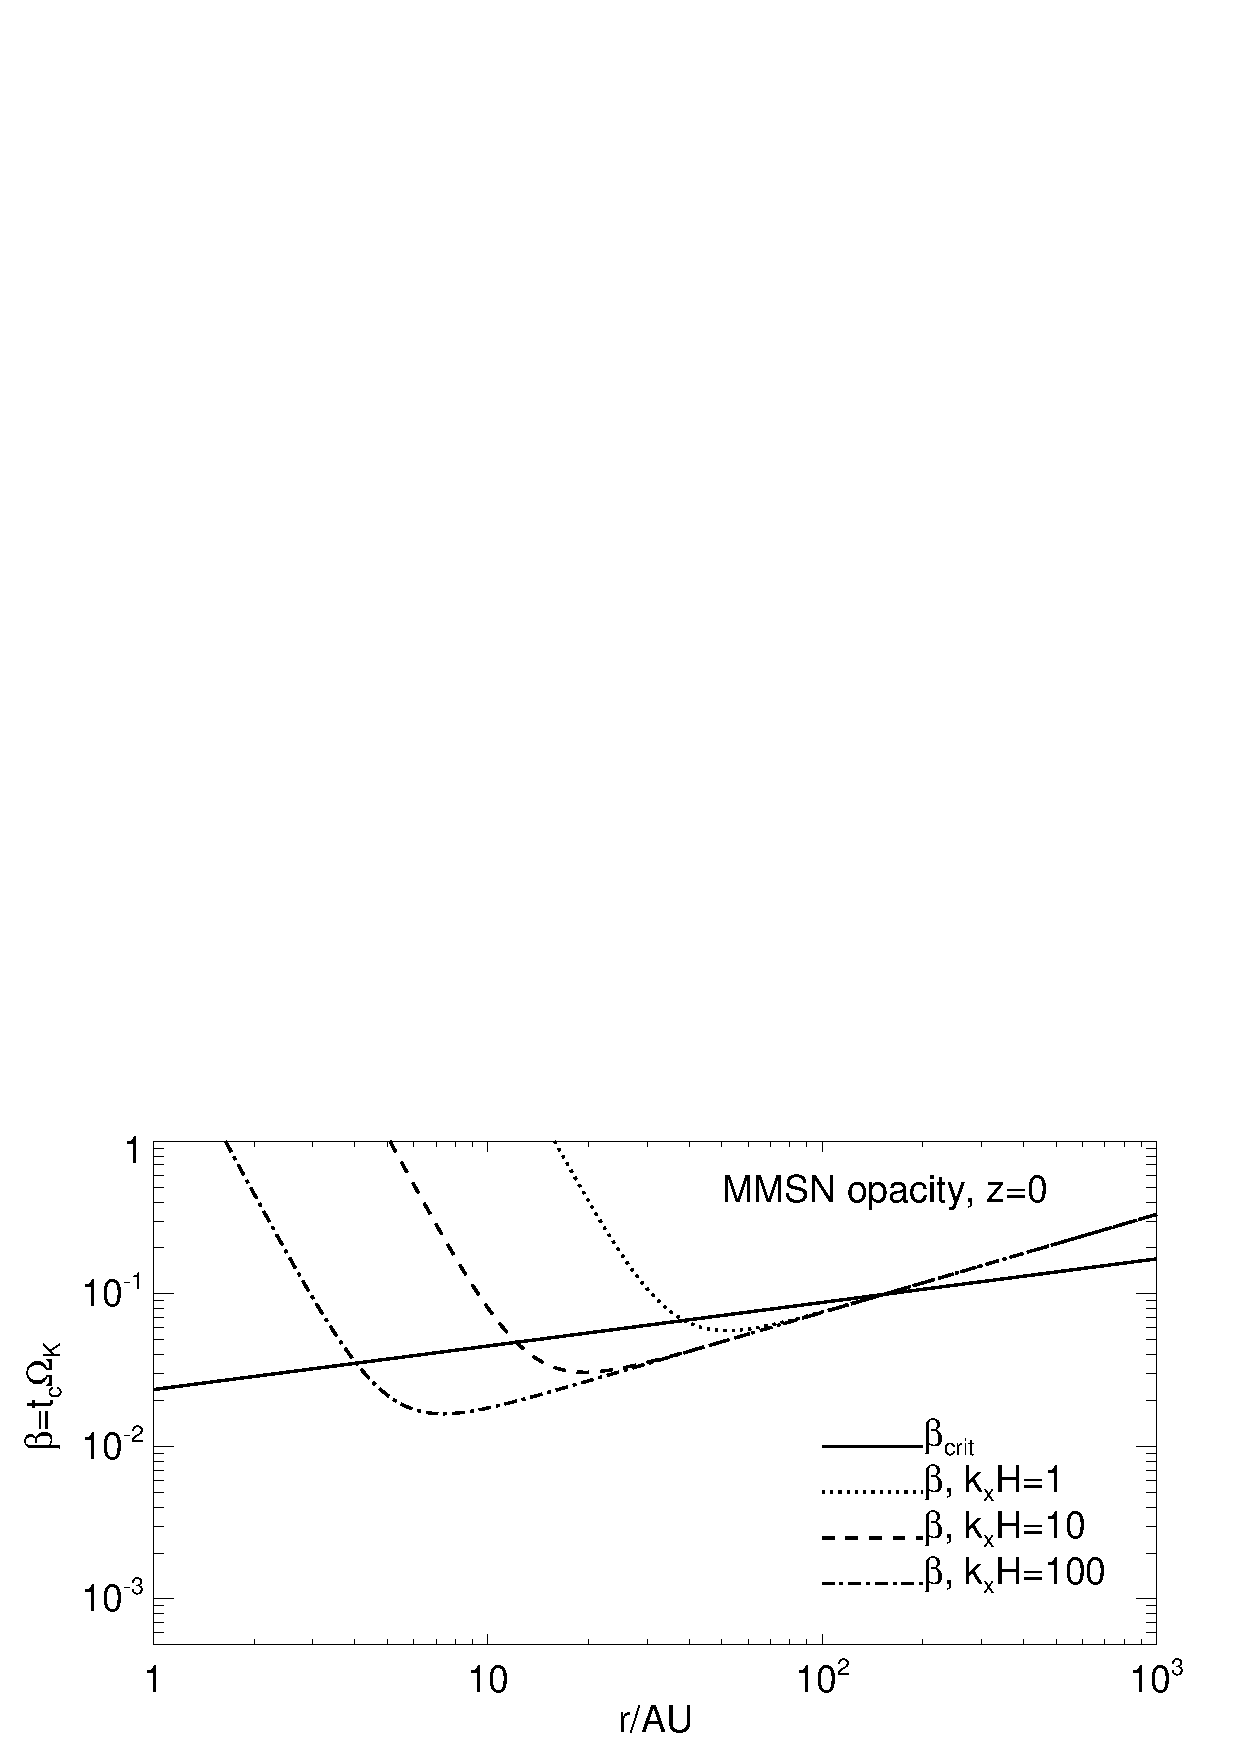
\includegraphics[scale=.47,clip=true,trim=0cm 1.8cm 0cm
  1cm]{figures/bcrit_mmsn_kap1_z0}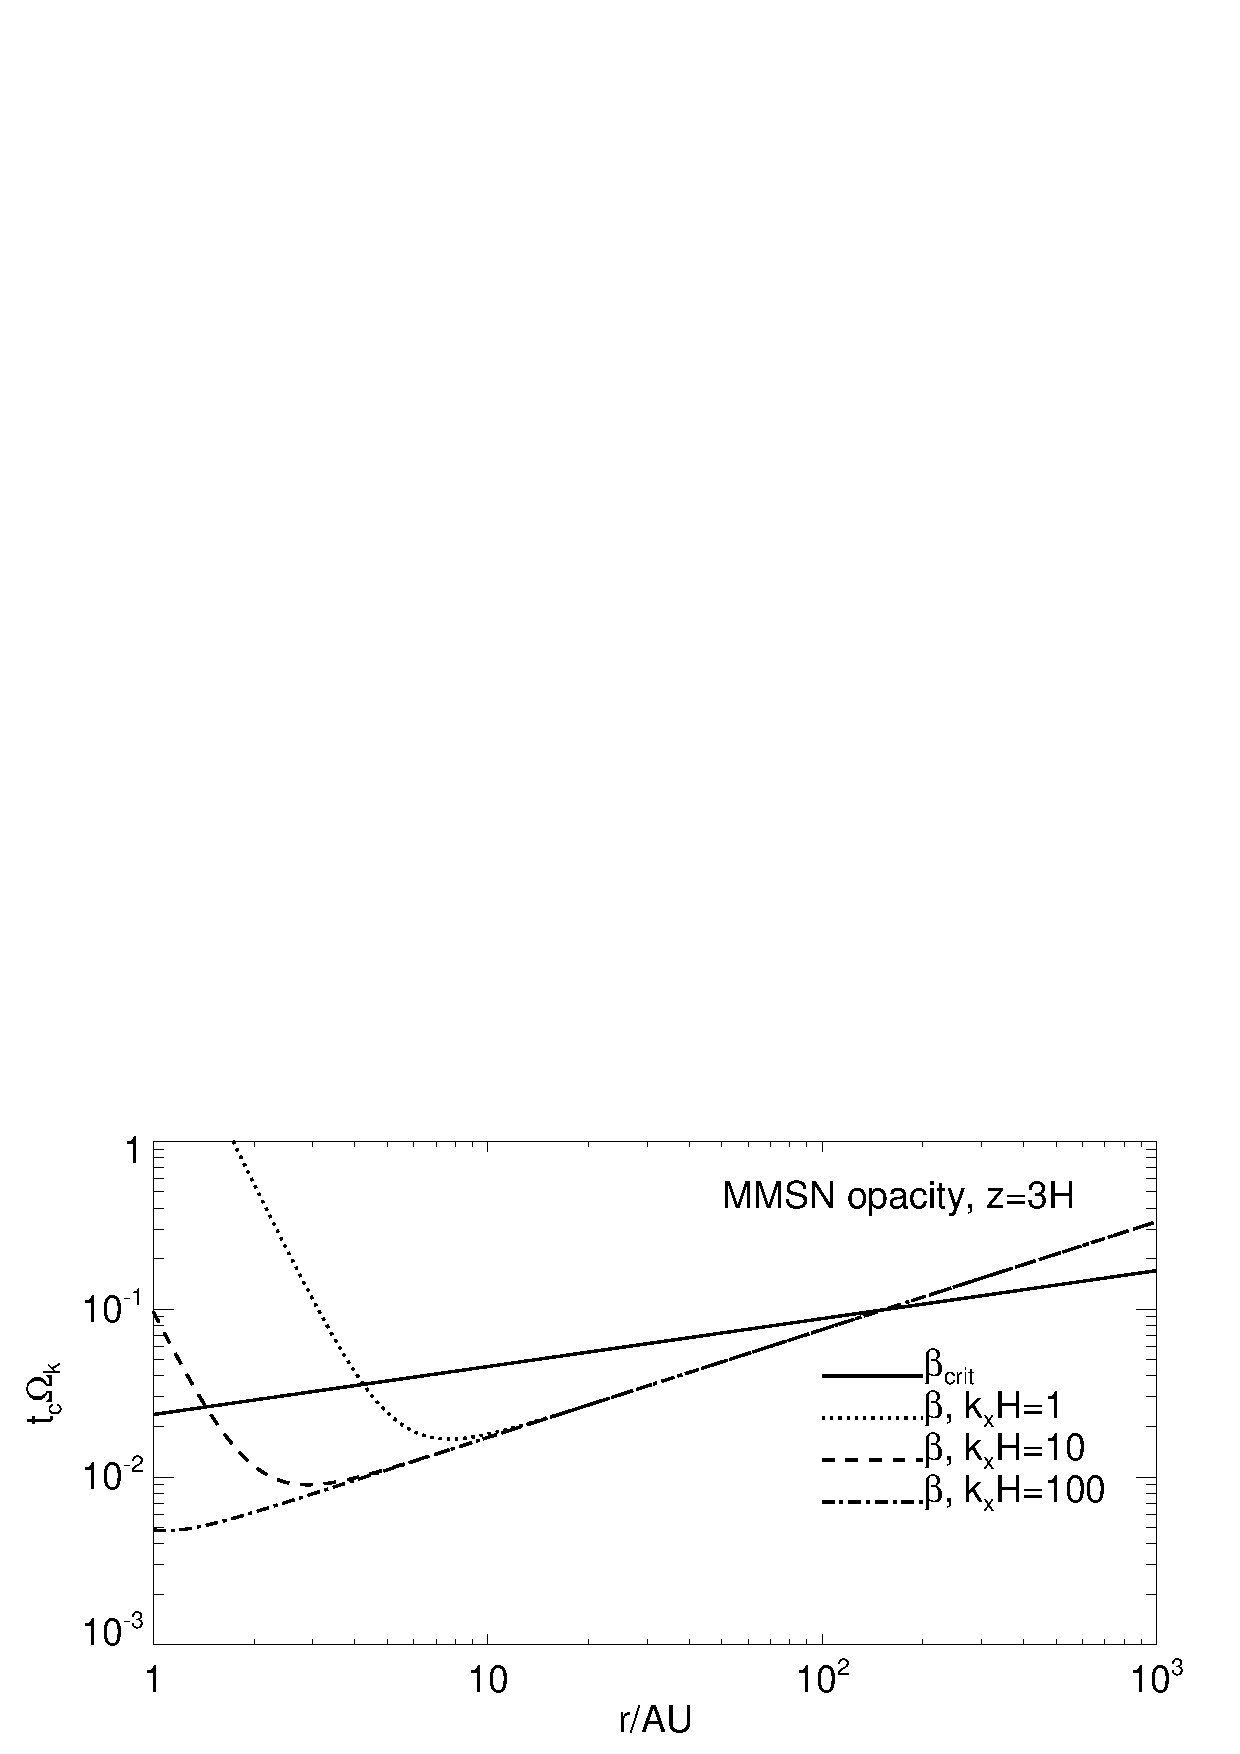
\includegraphics[scale=.47,clip=true,trim=2.5cm
  1.8cm 0cm 1cm]{figures/bcrit_mmsn_kap1_z3}\\
  \includegraphics[scale=.47,clip=true,trim=0cm 0cm 0cm
  1cm]{figures/bcrit_mmsn_kap10_z0}\includegraphics[scale=.47,clip=true,trim=2.5cm 0cm 0cm
  1cm]{figures/bcrit_mmsn_kap10_z3} 
  \caption{Dimensionless thermal relaxation timescales $\beta$,
    evaluated at the midplane (left) and at $z=3H$ (right) in the
    fiducial protoplanetary disk. Eq. \ref{beta_mmsn} is plotted  
    for three values of the 
    perturbation radial wavenumber: $\khat=1$ (dotted), $\khat=10$
    (dashed) and $\khat=100$ (dashed-dot), for three values of the
    opacity relative to the MMSN: $\hat{\kappa}_d=0.1$ (top),
    $\hat{\kappa}_d=1$ (middle) and $\hat{\kappa}_d=10$ (bottom).  
    The solid line is the 
    critical thermal relaxation timescale $\beta_\mathrm{crit}$.  
    \label{mmsn_bcrit_bcool}}   
\end{figure*}  

We remark that it is possible to satisfy $\beta < \beta_\mathrm{crit}$
for sufficiently large $\khat$. We
illustrate this in Fig. \ref{mmsn_bcrit_bcool_mink} by plotting at 
each radius the value of $\khat$ such  
that $\beta = \beta_\mathrm{crit}$. We thus expect that the VSI would only
occur on very small radial scales in the inner disk. 

However, disturbances with large $\khat$ may be subject to viscous
decay in a real disk. The viscous timescale for a perturbation lengthscale 
$l\sim 1/k_x$ is $t_\mathrm{visc} = 1/\alpha_s\khat^2\Omega $, where
$\alpha_s$ is the standard alpha viscosity parameter
\citep{shakura73}. Setting $t_\mathrm{visc}$ to be longer than the
minimum VSI growth timescale $1/\epsilon\Omega$ implies 
$\khat^2\lesssim \epsilon/\alpha_s$. Inserting $\epsilon \sim 0.05$,
we find only modes with $\khat\lesssim 20$ are relevant for
$\alpha_s\sim 10^{-4}$ or $\khat\lesssim 70$ for $\alpha_s\sim
10^{-5}$. \citep[These low viscosity levels are required for the
VSI, see][]{nelson13}.


\begin{figure}
  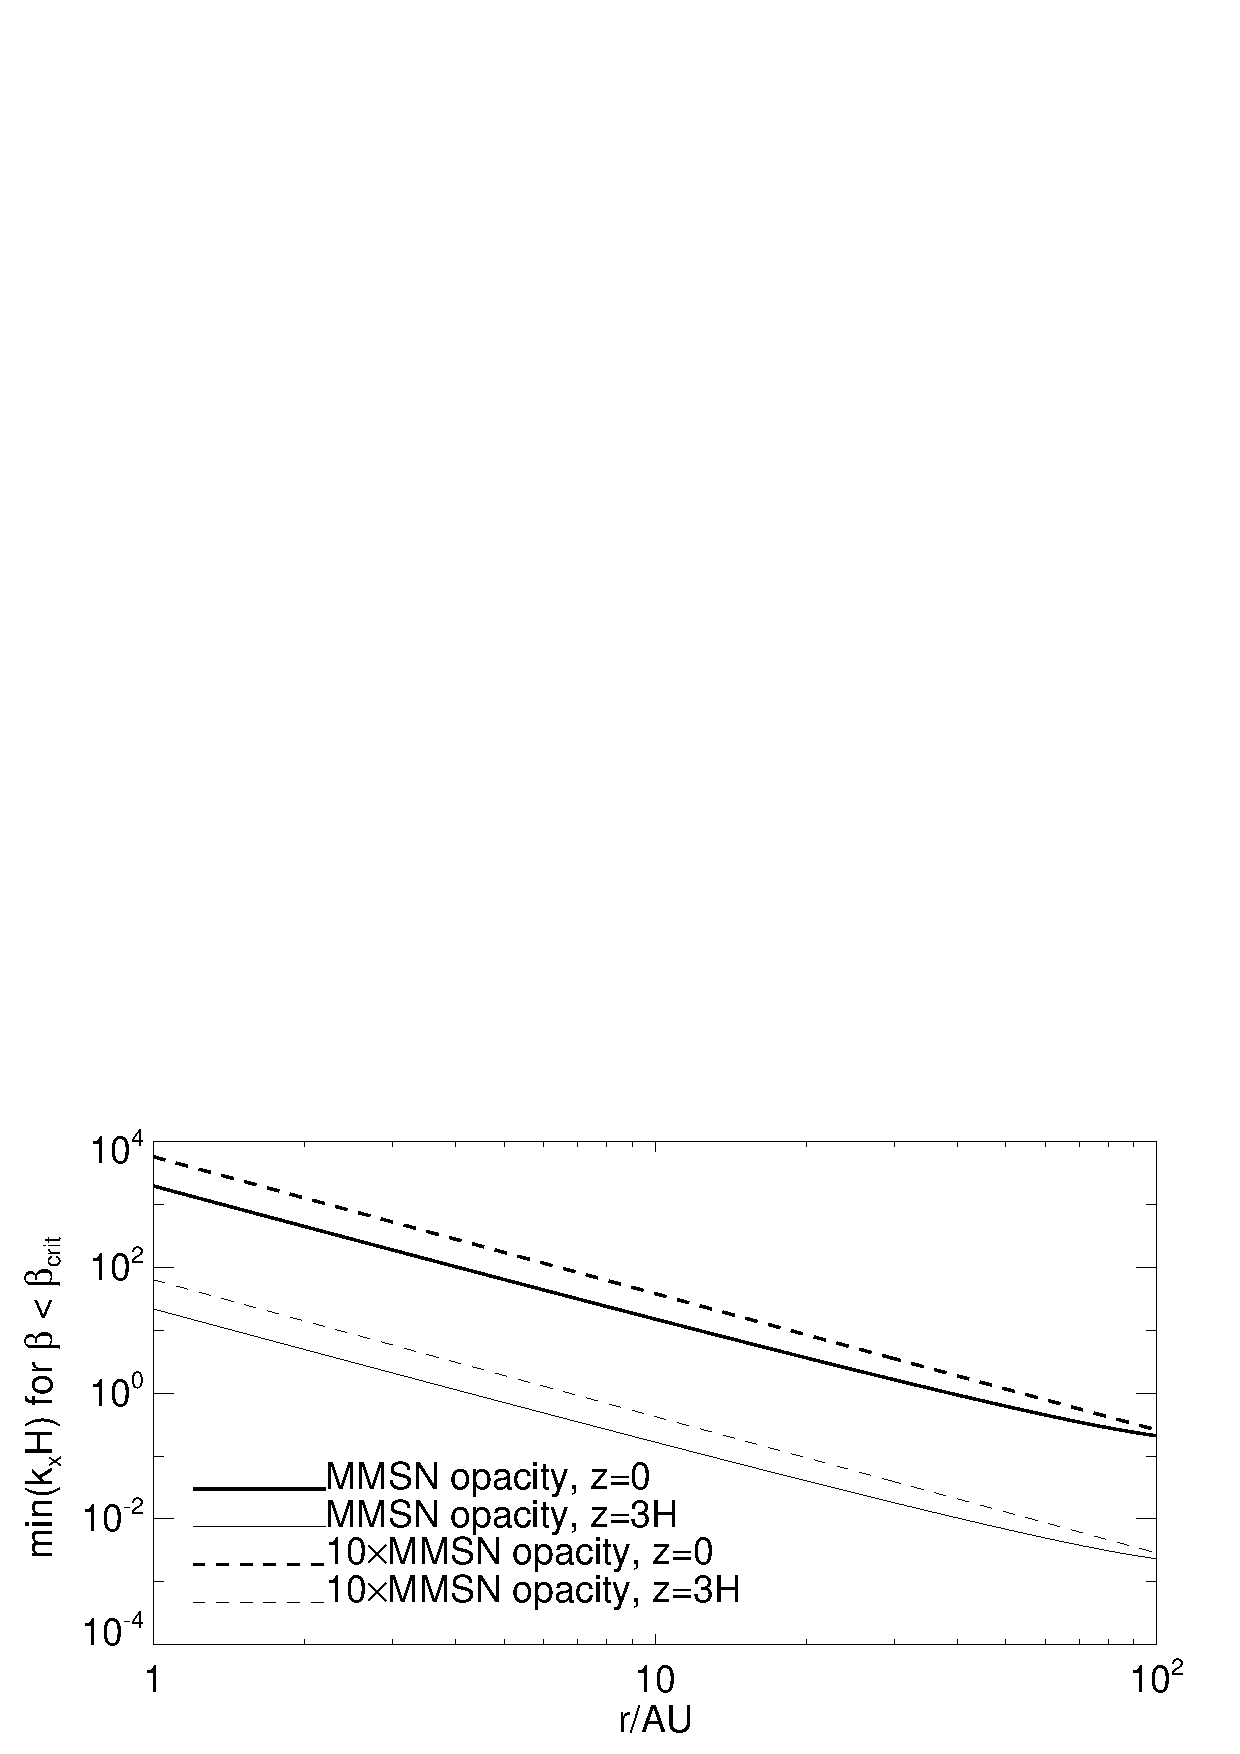
\includegraphics[width=\linewidth]{figures/bcrit_mink} 
  \caption{The minimum perturbation wavenumber $\khat$ in
    the MMSN such that the associated dimensionless thermal
    relaxation time  $\beta$ at $z=0$ (solid) and $z=3H$ (dashed) is
    less than the critical timescale $\beta_\mathrm{crit}$.   
    \label{mmsn_bcrit_bcool_mink}}   
\end{figure}  


\subsection{VSI in the MMSN}
Here we solve the linear stability problem in the MMSN with the scale and
height dependent thermal relaxation timescale given by
Eq. \ref{beta_mmsn_simp}.  Fig. \ref{beta_compare} show examples of
the thermal timescales at $r=5$AU and $r=50$AU for a
perturbation wavenumber $\khat=30$. We also plot the 
corresponding critical thermal timescales evaluated for the MMSN
(Eq. \ref{bcrit_mmsn}).  
 \begin{figure}
  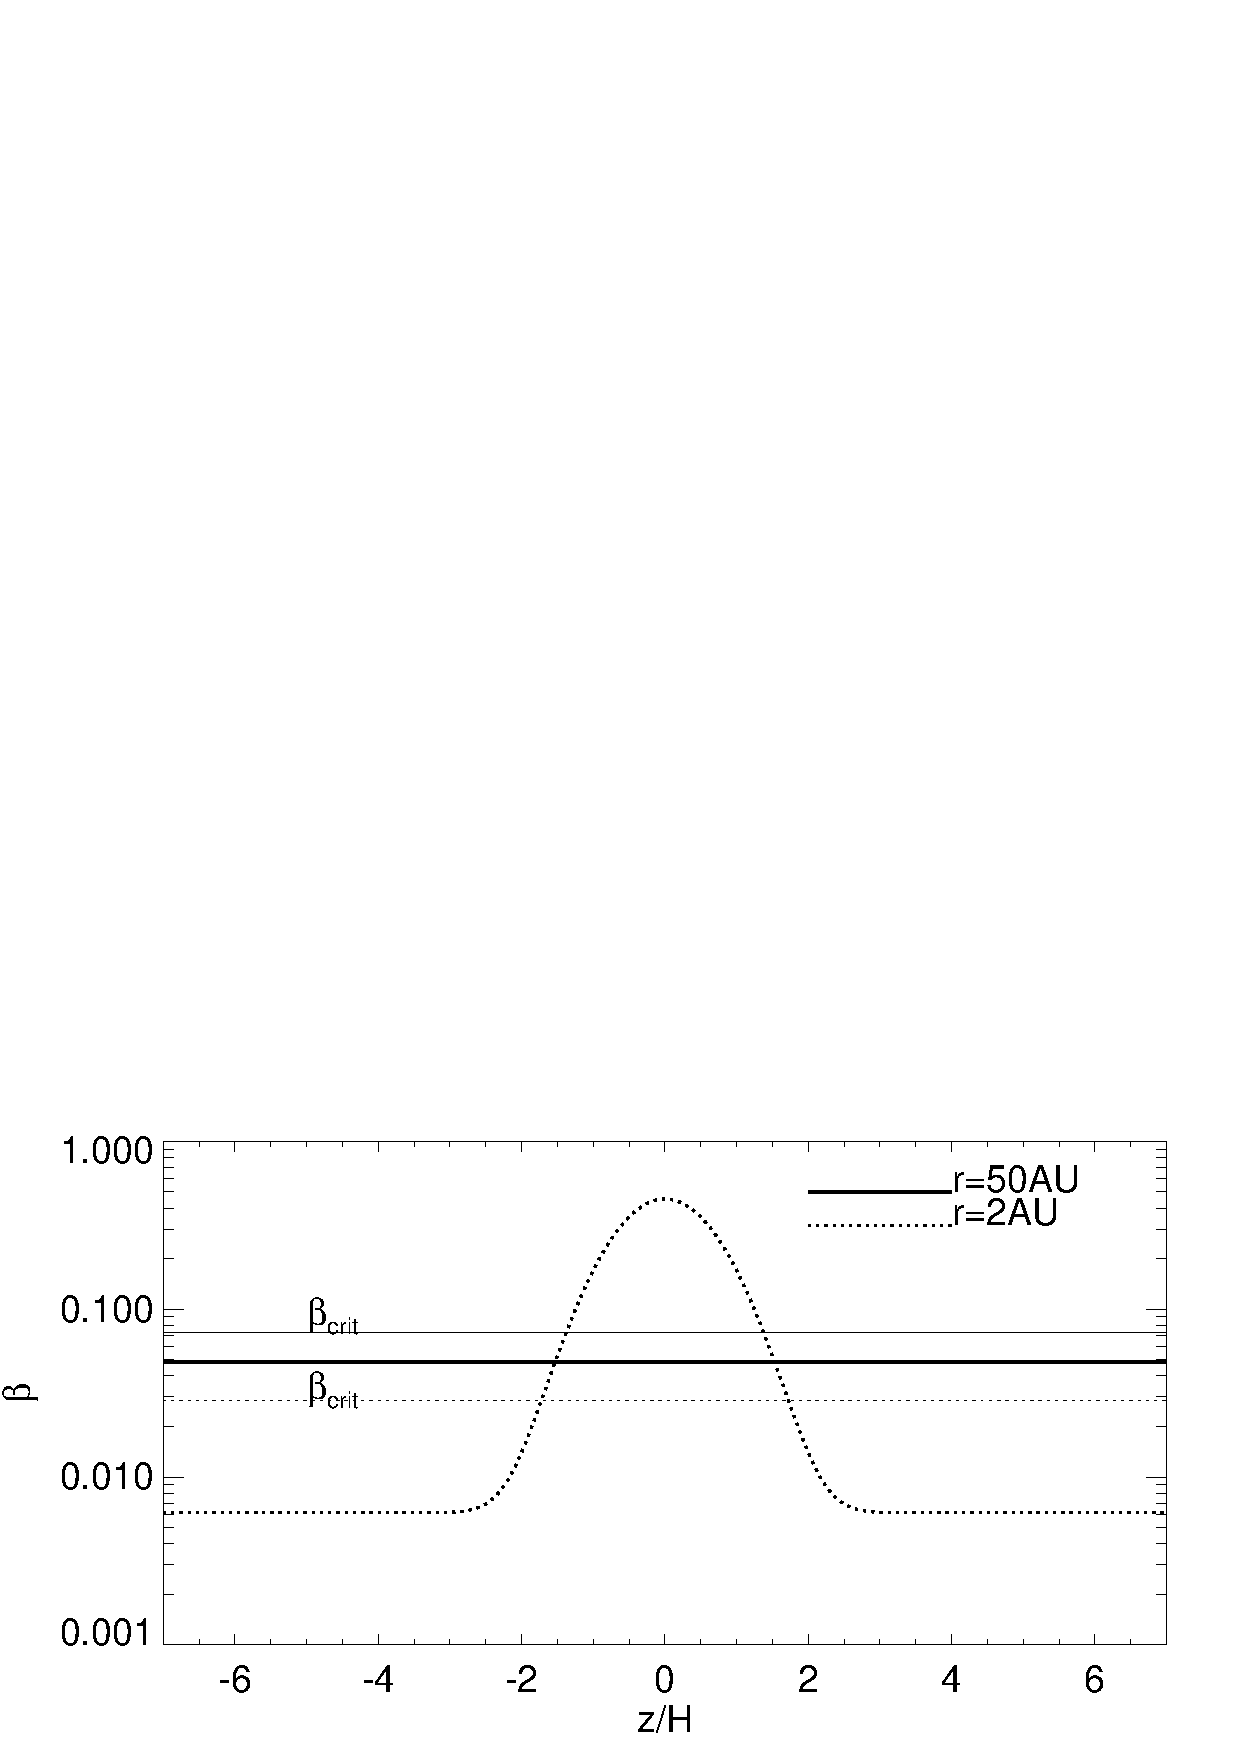
\includegraphics[width=\linewidth,clip=true,trim=0cm 0cm 0cm
  0cm]{figures/beta_compare}
  \caption{Thermal relaxation timescales in the MMSN at $r=50$AU
     and $r=5$AU for $\khat=30$ (solid lines). The
    corresponding horizontal dashed lines are the critical thermal
    relaxation timescales derived in linear theory. 
    \label{beta_compare}}
\end{figure}

The outer disk ($r=50$AU) is optically thin,
$\beta<\beta_\mathrm{crit}$  and  does not depend on height.
Accordingly we expect, and find, the VSI operates at $r=50$AU. The
inner disk ($r=5$AU) is optically thick near the midplane but becomes
optically thin away from it, such that $\beta < \beta_\mathrm{crit}$
for $|z|\gtrsim1.25H$. In fact, we also find the VSI in this case, but
with much reduced growth rates (when scaled by the local rotation), as
described below.     

In Fig. \ref{mmsn_overall} we plot characteristic growth timescales
$t_\mathrm{grow} \equiv 1/\nu$ of the fundamental mode with a range of
wavenumbers, in units of the local orbital time $P_\mathrm{orb}\equiv
2\pi/\Omega_k$.  In fact, we either only find the fundamental mode, or
that it is the most unstable, except for the appearance of some
surface modes towards the inner disk when considering large
wavenumbers $\khat\gtrsim 50$. However,
surface modes are affected by boundary conditions and disturbances
with large $\khat$ are more likely subject to viscous decay, as
discussed above. The dominance of the fundamental mode is also
observed in hydrodynamic simulations of \cite{stoll14} which treat
radiative cooling properly.   

We can therefore consider Fig. \ref{mmsn_overall} as a representation of the
VSI in the MMSN. We see the VSI operates from $\sim 5$AU to $\sim
50$AU with growth timescales $\sim 30$---40 orbits. It is necessary to
consider smaller scales with decreasing $r$ as the disk generally becomes
optically thick, and growth times rise rapidly towards the inner disk. 

The fact that we obtain the VSI in the inner disk despite $\beta >
\beta_\mathrm{crit}$ near the midplane suggests that the instability
can operate provided $\beta < \beta_\mathrm{crit}$ for a sufficiently large
fraction of the vertical domain. However, the normalized growth times
become much longer. For example, for $\khat=30$ we find
$t_\mathrm{grow}\sim 40$ orbits at $r=50$AU, but $t_\mathrm{grow}\sim
400$ orbits at $r=5$AU. Thus, introducing an optically thick midplane
significantly reduces the efficiency of the VSI despite $\beta <
\beta_\mathrm{crit}$ away from the midplane. 

We thus find Fig. \ref{mmsn_overall} to be roughly consistent with
comparing the midplane thermal relaxation timescales to the critical
thermal timescale. For example, 
Fig. \ref{mmsn_bcrit_bcool} show that $\beta(\khat=10,z=0) \gtrsim
\beta_\mathrm{crit}$ for $r\lesssim 10$AU in the MMSN (left middle panel); and Fig. \ref{mmsn_overall}
show that modes with $\khat=10$ are stabilized inside $\sim 8$AU (where
$t_\mathrm{grow}\to\infty$). Our numerical results suggest the VSI
is efficient at radii of few tens of AU in the MMSN, consistent with
estimates made by \cite{nelson13}. 

\begin{figure}
  \includegraphics[width=\linewidth]{figures/eigen_compare_grow.ps}
  \caption{Characteristic growth times of the VSI in 
    the MMSN. These are calculated using the scale and height
    dependent thermal relaxation given by Eq. \ref{beta_mmsn_simp}. 
    \label{mmsn_overall}}    
\end{figure} 
\section{Summary and discussion}\label{summary}
In this paper we have studied the  axisymmetric vertical shear
instability (VSI) in astrophysical disks that arises from the
height dependence of the equilibrium angular velocity profile
$\Omega=\Omega(r,z)$ in a baroclinic disk. We examined how
the linear instability depends on disk thermodynamics and applied our
results to assess the relevance of the VSI in realistic protoplanetary
disks.  

We generalized previous vertically global linear 
calculations of the VSI \citep{nelson13,mcnally14}, which assumed isothermal
perturbations, to include an energy equation. Our effort may also be
regarded as an extension of \cite{urpin03}, which did include an
energy equation, by relaxing the Boussinesq and vertically local
approximations adopted in that analysis.      

We included a source term in the energy equation which relaxes the disk
temperature to its initial value on a timescale
$t_c=\beta\Omega_k^{-1}$. This approach allows the thermodynamic
response of the disk to be controlled by varying the parameter
$\beta$, and has been employed in previous numerical simulations of
the VSI \citep{nelson13}. However, it is possible to 
relate  $\beta$ to physical thermal timescales expected in realistic disks.  

In accordance with the above studies, which show that the VSI occurs for 
perturbations with small radial lengthscales, we applied the 
radially local approximation in the linearized fluid equations. For
analytic discussion only, we further simplified the linear problem by
ignoring the background radial disk structure. This is equivalent to adopting
the `vertically-global shearing box' (VGSB) formalism developed by
\cite{mcnally14}. % who showed the linear VSI studied by
% \cite{nelson13} in a locally isothermal disk can be captured by the
% VGSB. 
We find the VGSB framework is appropriate for non-isothermal
perturbations provided $\beta\lesssim1$.  This is convenient because
rapid thermal relaxation ($\beta\ll1$) is 
generally required for the VSI.  However, the VGSB framework is not
appropriate in the adiabatic limit ($\beta \gg 1$). 
   
%OK framework for the regime of interest 
% The presence of a
% vertical shear, but 
% is not consistent with the
% global 

We mostly focused on vertically isothermal disks ($\Gamma=1$) as 
this is the relevant case for protoplanetary disks that are passively irradiated by its central star 
\citep{chiang97}. It also permits a largely analytical discussion.
Our analysis is an extension of the linear models considered in
\cite{lubow93} by  adding vertical shear and (rapid) thermal
relaxation. We obtained explicit solutions describing the VSI with 
thermal relaxation in the thin disk limit. 

The fundamental VSI mode is characterized by a symmetric vertical
velocity perturbation with zero nodes and $\delta
v_z\sim\mathrm{constant}$ near the mid-plane, and by an anti-symmetric
density perturbation with one node at $z=0$.  These have been referred
to as `corrugation modes' by \cite{nelson13}, and were found to
dominate their numerical simulations, as well as that of
\cite{stoll14}. Furthermore, when computing unstable modes for a
protoplanetary disk model with thermal relaxation based on realistic
disk properties, we find the fundamental mode to be the dominant
mode. The fundamental mode is
thus likely the most relevant VSI mode in protoplanetary disks.  

We determined the critical thermal relaxation timescale 
$\beta_\mathrm{crit}=\epsilon|q|/(\gamma-1)$, below which small-scale
perturbations may be regarded as isothermal and the VSI 
operates. We have therefore provided a quantitative measure for the `fast'
thermal relaxation requirement for the VSI in astrophysical disks. 

We also solved the linear stability problem numerically using a
pseudo-spectral approach. For numerical calculations we relax all the
approximations made in our analysis, and accounted for
the background radial disk structure.  Our
numerical results are mostly consistent with our analytic 
expectations, including the dependence of $\beta_\mathrm{crit}$ on
disk parameters.  We find the fundamental mode is robust against
boundary conditions, and higher order modes are more rapidly
stabilized with increasing $\beta$. 

We briefly studied vertically non-isothermal disks using our linear 
code. We confirm the finding by \cite{nelson13} that in the absence
of vertical entropy gradients, the VSI does not require rapid thermal
relaxation.  When a stable stratification is introduced, the
rapid reduction in VSI growth rates by a finite thermal relaxation
timescale is qualitatively similar to that observed for vertically
isothermal disks. Based on numerical results, we conjecture that the
critical thermal relaxation timescale is given by 
$\beta_\mathrm{crit}=\epsilon|q|/(\gamma-\Gamma)$ in vertically 
non-isothermal disks.  

%application to MMSN 

We applied our linear models to assess the applicability of the VSI in
protoplanetary disks. We considered the Minimum Mass Solar Nebulae
(MMSN) described in \cite{chiang10} and   
modeled the thermal relaxation timescale $\beta$ based on realistic
disk properties and dust opacity. This results in a $\beta$ function that
depends on both the perturbation lengthscale as well as the height 
from the midplane. We find the MMSN is unstable to the VSI 
from $\sim 5$AU to $\sim50$AU with characteristic growth times of
$\sim 30$ orbits. Although $\beta$ is not vertically constant in the
MMSN as assumed in our analysis, we find that evaluating the condition
$\beta <\beta_\mathrm{crit}$ at the disk midplane gives a rough measure of the
radii at which the VSI operates in the MMSN. This simple criteron is
thus a useful first step to estimate the relevance of the VSI in
realistic astrophysical disks without resorting to non-linear
numerical simulations.  

\subsection{Caveats and outlooks} 
We highlight below some extensions to the present  
linear models in future works.  

\subsubsection{Convective overstability}
We have focused on parameter regimes relevant to the VSI,
namely $\khat\gtrsim 1$ and $\beta\ll 1$. This excludes the
`convective overstability' recently discussed by \cite{klahr14} and
\cite{lyra14} in vertically unstratified disk models. 

The convective overstability corresponds to slowly growing epicyclic motions.
It is most effective for $\beta\sim 1$ and disturbances with $|k_x|\ll |k_z|$, where
$k_z$ is a vertical wavenumber. These conditions are mutually exclusive with the VSI. 
The maximum growth rate for convective overstability is given by 
\begin{align}
  \nu_\mathrm{conv,max} = -\frac{N^2_r}{4\Omega}\label{max_conv_gen}
\end{align}
\citep{lyra14}, where $N_r^2 = -(c_p\rho)^{-1}\p_rP\p_rS$ is the
square of the radial buoyancy frequency
(cf. Eq. \ref{nzsq_def}). Thus, growth requires $N_r^2<0$.  

Evaluating Eq. \ref{max_conv_gen} at the midplane of our disk models,
we find  
\begin{align}
  \nu_\mathrm{conv,max} =
  -\frac{\epsilon^2\Omega_k}{4\gamma\Gamma}\left(p+q\right)
  \left[\left(\gamma-1\right)p-q\right]. \label{max_conv}
\end{align}
In fact, for the MMSN considered in this work, convective
overstability does not apply because 
$N_r^2>0$.   

For more general disk structures convective overstability is
possible. The models adopted for our numerical study in
\S\ref{numerical} do satisfy $N_r^2<0$, but convective overstability
requires considering perturbations with long radial lengthscales,
$\khat\ll 1$, for which radially global disk models would be more 
appropriate.  

\subsubsection{Improved thermal evolution} 
We assumed non-adiabatic effects
can be represented by a thermal relaxation or cooling timescale $t_c$. For 
application to protoplanetary disks we connected $t_c$ to the disk
properties. One can improve the realism further by generalizing the 
opacity model adopted here to be density (and hence height) dependent. 
%here to be density-dependent,  i.e. $\kappa_d =
%% \kappa_d(\rho, T)$. 
However, going beyond thermal relaxation requires a
proper treatment of radiative diffusion. The linear problem then
involves a Laplacian operator, which require additional boundary
conditions. We will consider these improvements in a
follow-up study. %additional heat source 
 
\subsubsection{Additional physics} 
Depending on where the VSI operates in a
disk, additional effects may become important. For example, in the
outer parts of a protoplanetary disk, where we estimate the VSI 
operates, disk self-gravity (SG) may play a role. Vertical
self-gravity may favor the VSI by increasing $|\p_z\Omega|$ through
enhancing the density stratification 
(Eq. \ref{vertical_shear}). %sg in pert? no because kx>>1. but maybe for kx~1 

We have neglected viscosity. \cite{nelson13} find that an 
alpha viscosity $\lesssim O(10^{-4})$ is required for the VSI. 
It is of interest to quantify the effect of viscosity 
on the linear VSI. This would help identify, more accurately, the
appropriate regions in a protoplanetary disk that are sufficiently
laminar to develop the VSI.  This problem is, however, complicated by
the fact that proper inclusion of viscosity introduces a meridional
flow in the equilibrium state, as well as viscous heating
in the energy equation. 




\appendix
\section{Local model for a global problem}
Here, we discuss the relation between the linear problem in the
VGSB framework and the global linear problem. We begin with the
axisymmetric linearized fluid equations in cylindrical co-ordinates, including
thermal relaxation, 
\begin{align}
\ii\sigma\delta P &=\frac{\p P}{\p z}\delta v_z + \gamma P
\left[\frac{1}{r}\frac{\p}{\p r}\left(r\delta v_r\right) + \frac{\p
    \delta v_z}{\p z}\right] + \frac{1}{t_c}\left(\delta P -
  \frac{P}{\rho}\delta\rho\right) + \hat{g}_c \frac{\p P}{\p r}\delta v_r,\\
  \ii\sigma\delta\rho &= \frac{\rho}{r}\frac{\p}{\p r}\left(r\delta v_r\right) + \frac{\p}{\p
  z}\left(\rho\delta v_z\right)  + \hat{g}_c\frac{\p\rho}{\p r}\delta v_r,\\
\ii\sigma\delta v_r &= \frac{1}{\rho}\frac{\p\delta P}{\p r} - 2\Omega
\delta v_\phi - \hat{g}_c\frac{\delta\rho}{\rho^2}\frac{\p P}{\p r},\\ 
\ii\sigma\delta v_\phi  &= \frac{\kappa^2}{2\Omega}\delta v_r +
r\frac{\p\Omega}{\p z}\delta v_z,\\
\ii \sigma\delta v_z &= \frac{1}{\rho}\frac{\p\delta P}{\p z} -
\frac{\delta \rho}{\rho^2}\frac{\p P}{\p z},
\end{align}
where the coefficients $\hat{g}_c=1$ are inserted to label terms
associated with the background radial disk structure. 

We assume perturbations have the form $W(z)\exp{\ii k_r r}$ such
that $|k_rr|\gg1$, so that curvature terms can be ignored. For these
small radial lengthscale perturbations we also approximate the
background structure and radial gradients as uniform in $r$, and
evaluate all cofficients in the above equations at the fiducial radius
$r=r_0$. This procedure produces $\phi$ and $z$ momentum equations
that are equilvalent to those for $y$ and $z$ momenta in the VGSB. 

Using the notation and disk models in the main text, the
energy, density and $r$ momentum equations become 
\begin{align}
  \ii \sigma W  &=c _s^2(r_0, z)\left( \left.\frac{\p\ln\rho}{\p
      z}\right|_0 \delta v_z + \frac{\gamma}{\Gamma} \frac{d\delta
    v_z}{dz}\right) + \left[\ii k_rc_s^2(r_0,z)
  \frac{\gamma}{\Gamma} + \hat{g}_c\left.\frac{1}{\rho}\frac{\p P}{\p
      r}\right|_0\right]\delta v_r  +
\frac{1}{t_c}\left(W-\frac{Q}{\Gamma}\right),\\
\ii \sigma Q &= c_s^2(r_0,z)\left(\ii k_r + \hat{g}_c
  \left.\frac{\p\ln{\rho}}{\p r}\right|_0\right)\delta v_r + c _s^2(r_0, z)\left( \left.\frac{\p\ln\rho}{\p
      z}\right|_0 \delta v_z + \frac{d\delta
    v_z}{dz}\right), \\
\ii \sigma \delta v_r & = \ii k_r W  -
\hat{g}_c\frac{1}{c_s^2(r_0,z)}\left.\frac{1}{\rho}\frac{\p P}{\p
  r}\right|_0Q - 2\Omega(r_0,z)\delta v_\phi,
\end{align}
where subscript $0$ denotes evaluation at $r=r_0$. To obtain the
linear problem in the VGSB, we take the radially-local 
approximation further and formally set $\hat{g}_c=0$, and define the
new co-ordinate $x=r - r_0$ with $k_r\to k_x$. It is clear that
this approximation improves with increasing $|k_x|$. 

We may also reverse this procedure by reinstating the `global
correction' terms proportional to $\hat{g}_c$ in the linear VGSB
equations. Of course, doing so implies the basic state is not uniform
in $x$, which would be inconsistent with the full VGSB equations in
equilibrium. 
 
%nevertheless we have calculated
%plot growth rate v.s. bcool 




\section{Full governing equation for vertically isothermal disks}\label{adia_improve}
% \section{Improving the nearly-Keplerian approximation for adiabatic
%   disks}\label{adia_improve}
In \S\ref{approx_gov} we made the replacement $D\to\Omega_k^2$ before
eliminating variables to obtain a single equation for $\delta v_z$,
Eq. \ref{vertiso_gov}.  This procedure ignores the vertical dependence of
$D=\kappa^2(z) - \sigma^2$. We show here that this has no significant
consequence for thin disks. 

In the global disk with $\Gamma=1$ we have
\begin{align}\label{dkappa2}
  \frac{\p\kappa^2}{\p z} = 4 \frac{\p\Omega^2}{\p z} + r\frac{\p}{\p
    r}\frac{\p\Omega^2}{\p z} = -
  \frac{\p\ln\rho}{\p z}\frac{qc_s^2}{r^2} \left(2 + q +
    \frac{z^2/r^2-2}{z^2/r^2+1}\right). 
\end{align}
For the local problem we may then write
\begin{align}
  \frac{dD}{dz}  = - \frac{d\ln\rho}{dz}\frac{qc_s^2}{r^2}F(z;q),
\end{align}
where the function $F$ corresponds to the bracket in
Eq. \ref{dkappa2}. This function varies from $F=q$ at $z=0$ to $F\to
3+q$ as $|z|\to\infty$, i.e. its magnitude is of order unity. 

 Eliminating $W$ and $Q$ from Eq. \ref{ode_w}---\ref{ode_Q} and
 Eq. \ref{lin_vz} for vertically isothermal disks, retaining the
 vertical dependence of $D$ and including thermal relaxation, we
 obtain 
\begin{align}
  0 =& \frac{d^2\delta v_z}{dz^2} + \left[1 + \frac{\ii k_x c_s^2
      q}{Dr} - \frac{k_x^2c_s^2}{\left(k_x^2c_s^2 + \chi
        D\right)}\frac{qc_s^2F}{Dr^2}\right]\frac{d\ln\rho}{dz}\frac{d\delta
    v_z}{dz} \notag\\
  &+ \left\{\sigma^2\left(\frac{k_x^2}{D} +
      \frac{\chi}{c_s^2}\right) + \left(\chi + \frac{\ii k_x c_s^2
        q}{Dr}\right)\frac{d^2\ln\rho}{dz^2} -
    \frac{c_s^2}{D}\left(\frac{d\ln\rho}{dz}\right)^2\left(k_x^2 -
      \frac{\ii k_x q}{r}\right)
   \left[\left(1-\chi\right) +
     \frac{\chi}{\left(k_x^2c_s^2 + \chi D\right)}\frac{qc_s^2 F}{r^2}\right] 
   \right\}\delta v_z,
\end{align}
where we recall $\chi = \left(1-\ii\sigma t_c\right)/\left(1-\ii\sigma
t_c \gamma\right)$. Making the low-frequency approximation with the
replacement $D\to \Omega_k^2$ gives, in terms of dimensionless
variables,
\begin{align}
   &\delta v_z ^{\prime\prime} + \left[1 + \ii\epsilon q\hat{k} -
    \frac{ \hat{k}^2}{
      \left(\hat{k}^2+\chi\right)}q \epsilon^2F\right]\ln\rho^{\prime}\delta v_z^\prime +
  \left\{\left(\chi + \ii \epsilon q
      \hat{k}\right)\ln\rho^{\prime\prime} - \ln\rho^{\prime
      2}\left(\khat^2 -
      \ii\epsilon
      q\hat{k}\right)\left[1 - \chi +
      \frac{\chi}{\left(\hat{k}^2+\chi\right)}q\epsilon^2F\right]\right\}\delta v_z \notag\\&=
  -\hat{\sigma}^2\left(\hat{k}^2+\chi\right)\delta v_z\label{adia_diso3}.
\end{align}   
Eq. \ref{adia_diso3} differs from Eq. \ref{vertiso_gov_nondim} by terms
proportional to $\epsilon^2$. For a thin disk, $\epsilon\ll1$, so
neglecting these terms has no qualitative effect on the discussion in
\S\ref{analytic_adia} and \S\ref{analytic_relax}.  This issue does not
arise for isothermal perturbations discussed in \S\ref{iso_discuss}
since in that case we work with a governing equation for $W$ instead. 

\section{Alternative inference of instability in the presence of weak
  vertical shear}\label{pert_theory}
We can also investigate the destabilizing effect of vertical shear
without explicitly solving the full governing equation,
Eq. \ref{iso_ode3}. We first
consider a system with $q\equiv0$, for which the eigenfunctions are
Hermite polynomials and the real eigenfrequencies are known. We then
perturb this system by introducing a weak vertical shear ($|q|\ll1$)
and linearize the governing equation. This procedure is
\begin{align}   
  q \to 0 + \delta q,\quad
  W \to \He_n + \delta W,\quad
  \hat{\sigma} \to \hat{\sigma} + \delta\hat{\sigma}. 
\end{align}
%where for this exercise we restore $\sigma$ as the eigenfrequency. 

Linearizing the integral relation Eq. \ref{integral_relation1} in the
thin-disk limit, and taking the
imaginary part, we have
\begin{align}
  2\hat{\sigma}\imag(\delta\hat{\sigma})
  \left(1+\hat{k}^2\right) \int_{-\infty}^{\infty} w(\zhat)
  \He_n^2(\hat{z}) d\hat{z}
  = \delta q \epsilon \hat{k} 
  \int_{-\infty}^{\infty}
  w(\zhat)\hat{z}\He_n(\hat{z})\He_n^\prime(\zhat) d\hat{z}
\end{align}
Recognizing $\hat{z} = \He_1(\hat{z})$ and using $\He_n^\prime = n
\He_{n-1}$ we have
 \begin{align}
   2\hat{\sigma}\imag(\delta\hat{\sigma})
   \left(1+\hat{k}^2\right) \int_{-\infty}^{\infty} w(\zhat)
   \He_n^2(\hat{z}) d\hat{z}
   =\delta q \epsilon \hat{k} 
   \int_{-\infty}^{\infty}
   w(\zhat)\He_1(\hat{z})\He_n(\hat{z})n\He_{n-1}(\hat{z})d\hat{z}. 
 \end{align}

Finally, we evaluate the integrals using the results
\begin{align}
  \int_{-\infty}^{\infty}
  w(\xi) \He_k(\xi)\He_l(\xi) d\xi = \sqrt{2\pi}k!\delta_{kl} \quad
% \end{align}
\text{and} \quad
% \begin{align}
  \int_{-\infty}^{\infty}
  w(\xi) \He_m(\xi)\He_k(\xi)\He_l(\xi) d\xi =
  \frac{\sqrt{2\pi}m!k!l!}{(j-m)!(j-k)!(j-l)!}, 
\end{align}
where $j = (m+k+l)/2$. We then obtain
 \begin{align}
   2\hat{\sigma}\imag(\delta\hat{\sigma})
  \left(1+\hat{k}^2\right) = \delta q \epsilon \hat{k} n.
 \end{align}
Inserting the original eigenfrequency $\hat{\sigma} = \pm
\sqrt{n}(1+\hat{k}^2)^{-1/2}$ gives
\begin{align}
  \imag(\delta\hat{\sigma})= \pm \frac{1}{2}\delta q \epsilon
  \sqrt{n} \frac{\hat{k}}{\sqrt{1+\hat{k}^2}}. 
\end{align}
This result agrees with Eq. \ref{simple_growth} in the limit
$|q|\to0$. 
%for $n=1$, since the
%function $\He_1$ solves the governing equation exactly. 
For $\hat{k}\gg 1$ we have
\begin{align}
  \imag(\delta\hat{\sigma})\simeq \pm \frac{1}{2}\delta q \epsilon
  \sqrt{n} \sgn{\hat{k}}. 
\end{align}




% Differentiating Eq. \ref{adia_iso1} properly gives
% \begin{align}
%   \left(D + \gamma k_x^2 c_s^2\right)\frac{d\Delta}{dz}=& D
%   \frac{d^2\delta v_z}{dz^2} + k_x^2c_s^2\left[\frac{\gamma}{\left(D + \gamma k_x^2 c_s^2\right)}\frac{dD}{dz} + \ii
%     \frac{d\ln\rho}{dz}\left(\ii +
%       \frac{q}{k_xr}\right)\right]\frac{d\delta v_z}{dz}\notag\\
%   &+ \ii k_x^2 c_s^2 \left(\ii +
%       \frac{q}{k_xr}\right)\left[\frac{d^2\ln\rho}{dz^2} -
%       \frac{1}{\left(D + \gamma
%           k_x^2c_s^2\right)}\frac{dD}{dz}\frac{d\ln\rho}{dz}\right]\delta
%     v_z. \label{adia_diso1}
% \end{align}
% The terms that were ignored in deriving Eq. \ref{adia_iso3} are those
% proportional to $dD/dz$ in Eq. \ref{adia_diso1}. Now, in the global
% disk with $\Gamma=1$ we have
% \begin{align}\label{dkappa2}
%   \frac{\p\kappa^2}{\p z} = 4 \frac{\p\Omega^2}{\p z} + r\frac{\p}{\p
%     r}\frac{\p\Omega^2}{\p z} = -
%   \frac{\p\ln\rho}{\p z}\frac{qc_s^2}{r^2} \left(2 + q +
%     \frac{z^2/r^2-2}{z^2/r^2+1}\right). 
% \end{align}
% For the local problem we may then write
% \begin{align}
%   \frac{dD}{dz}  = - \frac{d\ln\rho}{dz}\frac{qc_s^2}{r^2}F(z;q),
% \end{align}
% where the function $F$ corresponds to the bracket in
% Eq. \ref{dkappa2}. This function varies from $F=q$ at $z=0$ to $F\to
% 3+q$ as $|z|\to\infty$, i.e. its magnitude is of order unity. 
% % We estimate the
% % importance of these terms by noting that 
% % \begin{align}
% %   \frac{dD}{dz}\equiv \frac{d\kappa^2}{dz} \simeq \frac{d\Omega^2}{dz}
% %   = - \frac{d\ln\rho}{dz}\frac{qc_s^2}{r^2},
% % \end{align}
% % for thin disks. 
% Eq. \ref{adia_diso1} becomes
% \begin{align}
% \left(D + \gamma k_x^2 c_s^2\right)\frac{d\Delta}{dz}=& D
%   \frac{d^2\delta v_z}{dz^2} - k_x^2c_s^2\frac{d\ln\rho}{dz}\left[ 1 - 
%       \frac{\ii q}{k_xr}  +  \frac{\gamma q c_s^2F}{r^2\left(D +
%         \gamma k_x^2 c_s^2\right)}\right]\frac{d\delta
%     v_z}{dz}\notag\\ 
%   &- k_x^2 c_s^2 \left(1 - 
%       \frac{\ii q}{k_xr}\right)\left[\frac{d^2\ln\rho}{dz^2} + 
%       \frac{qc_s^2F}{r^2\left(D + \gamma
%           k_x^2c_s^2\right)}\left(\frac{d\ln\rho}{dz}\right)^2\right]\delta
%     v_z. \label{adia_diso2}
% \end{align}
% Since $D\sim \Omega_k^2$ in the low-frequency limit, we 
% see from Eq. \ref{adia_diso2} that the neglected terms are
% $O(\epsilon^2)$. We can make this explicit by combining
% Eq. \ref{adia_diso1}---\ref{adia_diso2} and Eq. \ref{adia_iso2}, then
% set $D\to\Omega_k^2$. In terms of non-dimensional variables, the result
% is  
% \begin{align}
%    &\delta v_z ^{\prime\prime} + \left(1 + \ii\epsilon q\hat{k} -
%     \frac{\gamma q \epsilon^2\hat{k}^2F}{1+\gamma
%       \hat{k}^2}\right)\ln\rho^{\prime}\delta v_z^\prime +
%   \left[\left(\frac{1}{\gamma} + \ii \epsilon q
%       \hat{k}\right)\ln\rho^{\prime\prime} - \hat{k}^2\left(1 -
%       \frac{\ii\epsilon
%         q}{\hat{k}}\right)\left(\frac{\gamma-1}{\gamma} +
%       \frac{q\epsilon^2F}{1+\gamma\hat{k}^2}\right)\ln\rho^{\prime
%       2}\right]\delta v_z \notag\\&=
%   -\hat{\sigma}^2\left(\frac{1}{\gamma} + \hat{k}^2\right)\delta v_z\label{adia_diso3}.
% \end{align}   
% Eq. \ref{adia_diso3} differs from Eq. \ref{adia_iso3} by terms
% proportional to $\epsilon^2$. For a thin disk, $\epsilon\ll1$, so
% neglecting these terms has no qualitative effect on the discussion in
% \S\ref{analytic_adia}. 

\section{Coefficients for the dispersion relation for perturbations
with thermal relaxation}\label{relax_coeff}
The coefficients of the dispersion relation Eq. \ref{relax_disp} is
given by:
\begin{align}
  &c_0 = M(M+1)\widetilde{A}^2,\\
  &c_1 = \ii\beta\left\{\left(1-\gamma\right)\left[1 +
      \khat^2\left(1+2M\right)^2 - 4 \ii\epsilon q\khat M (M+1)\right] 
    - 2\widetilde{A}^2\gamma M (M+1)\right\},\\
  &c_2 = \left(\khat^2 + 1\right)\widetilde{A} + \beta^2\left\{(1-\gamma)\left[1
      + \gamma \khat^2(1+2M)^2 - 4\ii\epsilon q \khat \gamma M(M+1)
    \right]
    -\gamma^2 \widetilde{A}^2 M(M+1)
  \right\},\\
  &c_3 = \beta\left\{\epsilon q \khat + \gamma \left[\ii + \epsilon q
      k \left(1+2\khat^2\right)\right] - 3\ii - 2\ii
    \khat^2\right\},\\
  &c_4 =
  \beta^2\left(1+\gamma\khat^2\right)\left[\gamma\left(1-\ii\epsilon q
    \khat\right)-2\right] - \left(1+\khat^2\right)^2,\\
&c_5 = 2\ii\beta\left(1+\khat^2\right)\left(1+\gamma\khat^2\right),\\
&c_6 = \beta^2\left(1+\gamma\khat^2\right)^2.
\end{align}

\section{Fiducial model for a protoplanetary disk}\label{mmsn}
For results application in \S\ref{application} we use the disk model
described in \cite{chiang10}. This disk model orbits a Solar-mass star and 
has the surface density distribution
\begin{align}\label{mmsn_sigma}
  \Sigma = 2200
  \hat{\Sigma}\left(\frac{r}{\mathrm{AU}}\right)^{-3/2}\mathrm{g}\,\mathrm{cm}^{-2},  
\end{align}
and the temperature profile
\begin{align}\label{mmsn_temp}
  T = 120\hat{T}\left(\frac{r}{\mathrm{AU}}\right)^{-3/7} \mathrm{K},
\end{align}
which implies $q=-3/7$. In the above expressions, $\hat{\Sigma}$ and
$\hat{T}$ are dimensionless coefficients used to scale the model
relative to the MMSN. Their nomial values are unity. By assuming a
vertically isothermal disk, we deduce the disk aspect-ratio 
\begin{align}\label{mmsn_epsilon}
  \epsilon =
  3.36\times10^{-2}\left(\frac{\hat{T}}{\mu}\right)^{1/2}\left(\frac{r}{\mathrm{AU}}\right)^{2/7}, 
\end{align}
and the mid-plane density distribution 
\begin{align}
%  \rho_0 = 2.7\times10^{-9}
%  \hat{\Sigma}\left(\frac{r}{\mathrm{AU}}\right)^{-39/14}\mathrm{g}\,\mathrm{cm}^{-3},  
\rho_0 = 1.7\times10^{-9}
  \hat{\Sigma}\left(\frac{\hat{T}}{\mu}\right)^{-1/2}\left(\frac{r}{\mathrm{AU}}\right)^{-39/14}\mathrm{g}\,\mathrm{cm}^{-3},
\end{align}
which implies $p=-39/14$. 
%0.033576258
In addition, we
use the opacity model {\bf(reference?)}
 \begin{align}
   \kappa_d &= 2 \hat{\kappa}_d \left(\frac{T}{100\mathrm{K}}\right)^2
   \mathrm{cm}^2\,\mathrm{g}
    =
   2.88\hat{\kappa}_d\hat{T}^2\left(\frac{r}{\mathrm{AU}}\right)^{-6/7}\mathrm{cm}^2\,\mathrm{g}^{-1},   
 \end{align}
where the second equality follows from the model temperature profile
above, and $\hat{\kappa}_d$ has similar meaning as $\hat{\Sigma}$ and
$\hat{T}$. 


\bibliographystyle{apj}
\bibliography{ref}


\end{document}

